% Chapter, Section, Theorem, Corollary, Lemma, Definition, Table, Figure, {\bf
\chapter{Pushdown Automata}\label{ch-10}

In the earlier part of this text, the representation of languages via regular
grammars was a generative construct equivalent to the cognitive power of
deterministic finite automata and nondeterministic finite automata. Chapter \ref{ch-9}
showed that context-free grammars had more generative potential than did regular
grammars, and thus defined a significantly larger class of languages. This
chapter and the next explore generalizations of the basic automata construct
introduced in Chapter \ref{ch-1}. In Chapter \ref{ch-4}, we discovered that adding nondeterminism
did not enhance the language capabilities of an automaton. It seems that more
powerful automata will need the ability to store more than a finite amount of
state information, and machines with the ability to write and read from an
indefinitely long tape will now be considered. Automata that allow unrestricted
access to all portions of the tape are the subject of Chapter \ref{ch-11}. Such machines
are regarded to be as powerful as a general-purpose computer. This chapter will
deal with automata with restricted access to the auxiliary tape. One such device
is known as a \emph{pushdown automaton} and is strongly related to the
context-free languages.

\section{Definitions and Examples}\label{sec-10.1}

A language such as $\{\pmb{a}^n\pmb{b}^n|\ n \geq 1\}$ can be shown to be non-FAD
by the pumping lemma, which uses the observation that a finite-state control
cannot distinguish between an unlimited number of essentially different
situations. Deterministic finite automata could at best ``count'' modulo some
finite number; unlimited matching was one of the many things beyond the
capabilities of a finite-state control. One possible enhancement would be to
augment the automaton with a single integer counter, which could be envisioned
as a sack in which stones could be placed (or removed) in response to input\index{sack and stone machine|see{counting automaton}}. The
automaton would begin with one stone in the sack and process input much as a
nondeterministic finite automaton would. With each transition, the machine would
not only choose a new state, but also choose to add another stone to the sack,
remove an existing stone from the sack, or leave the contents unchanged. The
$\delta$ function is independent of the status of the sack; the sack is used
only to determine whether the automaton should continue to process input
symbols. Perhaps some sort of weight sensor would be used to detect when there
were stones in the sack, and the device would continue to operate as long as
stones were present; the device would halt when the sack is empty. If all the
symbols on the input tape happen to have been consumed at the time the sack
empties, the input string is \emph{accepted} by the automaton.

Such devices are called \emph{counting automata}\index{counting automaton} and are general enough
to recognize many non-FAD languages. A device to recognize $\{\pmb{a}^n\pmb{b}^n
|\ n \geq 1\}$ would need three states. The start state will transfer control to a
second state when an $\pmb{a}$ is read, leaving the sack contents unchanged. The
start state will have no valid moves for $\pmb{b}$, causing words that begin with
$\pmb{b}$ to be rejected since the input tape will not be completely consumed. The
automaton will remain in the second state in response to each $\pmb{a}$, adding a
stone to the sack each time an $\pmb{a}$ is processed. The second state will
transfer control to the third state upon receipt of the symbol $\pmb{b}$ and
withdraw a stone from the sack. The third state has no moves for $\pmb{a}$ and
remains in that state while removing a stone for each $\pmb{b}$ that is processed.
For this device, only words of the form $\pmb{a}^n\pmb{b}^n$ will consume all
the input just when the sack becomes empty.

Another type of counting automaton handles acceptance in the same manner as
nondeterministic finite automata. That is, if there is a sequence of transitions
that consumes all the input and leaves the device in a final state, the input
word is accepted (irrespective of the sack contents). As with NDFAs, the device
may halt prematurely if there are no applicable transitions (or if the sack
empties).

These counting automata are not quite general enough to recognize all
context-free languages. More than one type of ``stone'' is necessary in order
for such an automaton to emulate the power of context-free grammars, at which
point the order of the items becomes important. Thus, the sack is replaced by a
\emph{\Index{stack}},\index{tape!stack} a last-in, first-out (LIFO) list. The most recently added
item is positioned at the end called the \emph{top} of the stack. A newly added
item is placed above the current top and becomes the new top item as it is
\emph{pushed} onto the stack. The action of the finite-state control can be
influenced by the type of item that is on the top of the stack. Only the top
(that is, the most recently placed) item can affect the state transition
function; the device has no ability to reexamine items that have previously
been deleted (that is, have been \emph{popped}). The next item below the top of
the stack cannot be examined until the top item is popped (and that popped item
thereby becomes unavailable for later reinspection). As with counting automata,
an empty stack will halt the operation of this type of automaton, called a
\emph{\Index{pushdown automaton}}.

% Definition 10.1
\begin{dfn}\label{dfn-10.1}\index{nondeterministic pushdown automaton|see{NPDA}}\index{final state!for PDA}\index{alphabet!input}\index{alphabet!stack}
A \emph{(nondeterministic) pushdown automaton} (\Index{NPDA} or just
\Index{PDA}) is a septuple\linebreak$P=\langle\Sigma,\Gamma,S,s_0,\delta,B,F\rangle$,
where
\ \\
\begin{tabular}{l}
$\Sigma$ is the \emph{input alphabet}. \\
$\Gamma$ is the \emph{stack alphabet}. \\
$S$ is a finite nonempty set of \emph{states}. \\
$s_0$ is the \emph{\Index{start state}} ($s_0\in S$). \\
$\delta$ is the \emph{state transition function}, \\
\indent$\delta\text{: }S\times(\Sigma\cup\lambda)\times\Gamma\rightarrow$ the set
of finite subsets of $S\times\Gamma^*$. \\
$B$ is the \emph{bottom of the stack} symbol ($B\in\Gamma$). \\
$F$ is the set of \emph{final states} ($F\subseteq S$).
\end{tabular}
\end{dfn}

By the definition of alphabet (Definition \ref{dfn-1.1}), both $\Sigma$ and $\Gamma$ must
be nonempty. Figure \ref{fig-10.1} presents a conceptualization of a pushdown automaton.
As with an NDFA, there is a finite-state control and a read head for the input
tape, which only moves forward. The auxiliary tape also has a \Index{read/write head},
which not only moves forward, but can move backward when an item is popped. The
state transition function is meant to signify that, given a current state, an
input symbol being currently scanned, and the current top stack symbol, the
automaton may choose both a new current state and a new string of symbols from
$\Gamma^*$ to replace the top stack symbol. This definition allows the machine
to behave nondeterministically, since a current state, input letter, and stack
symbol are allowed to have any (finite) number of alternatives for state
transitions and strings from $\Gamma^*$ to record on the stack.

% Figure 10.1
\begin{figure}
\centerline{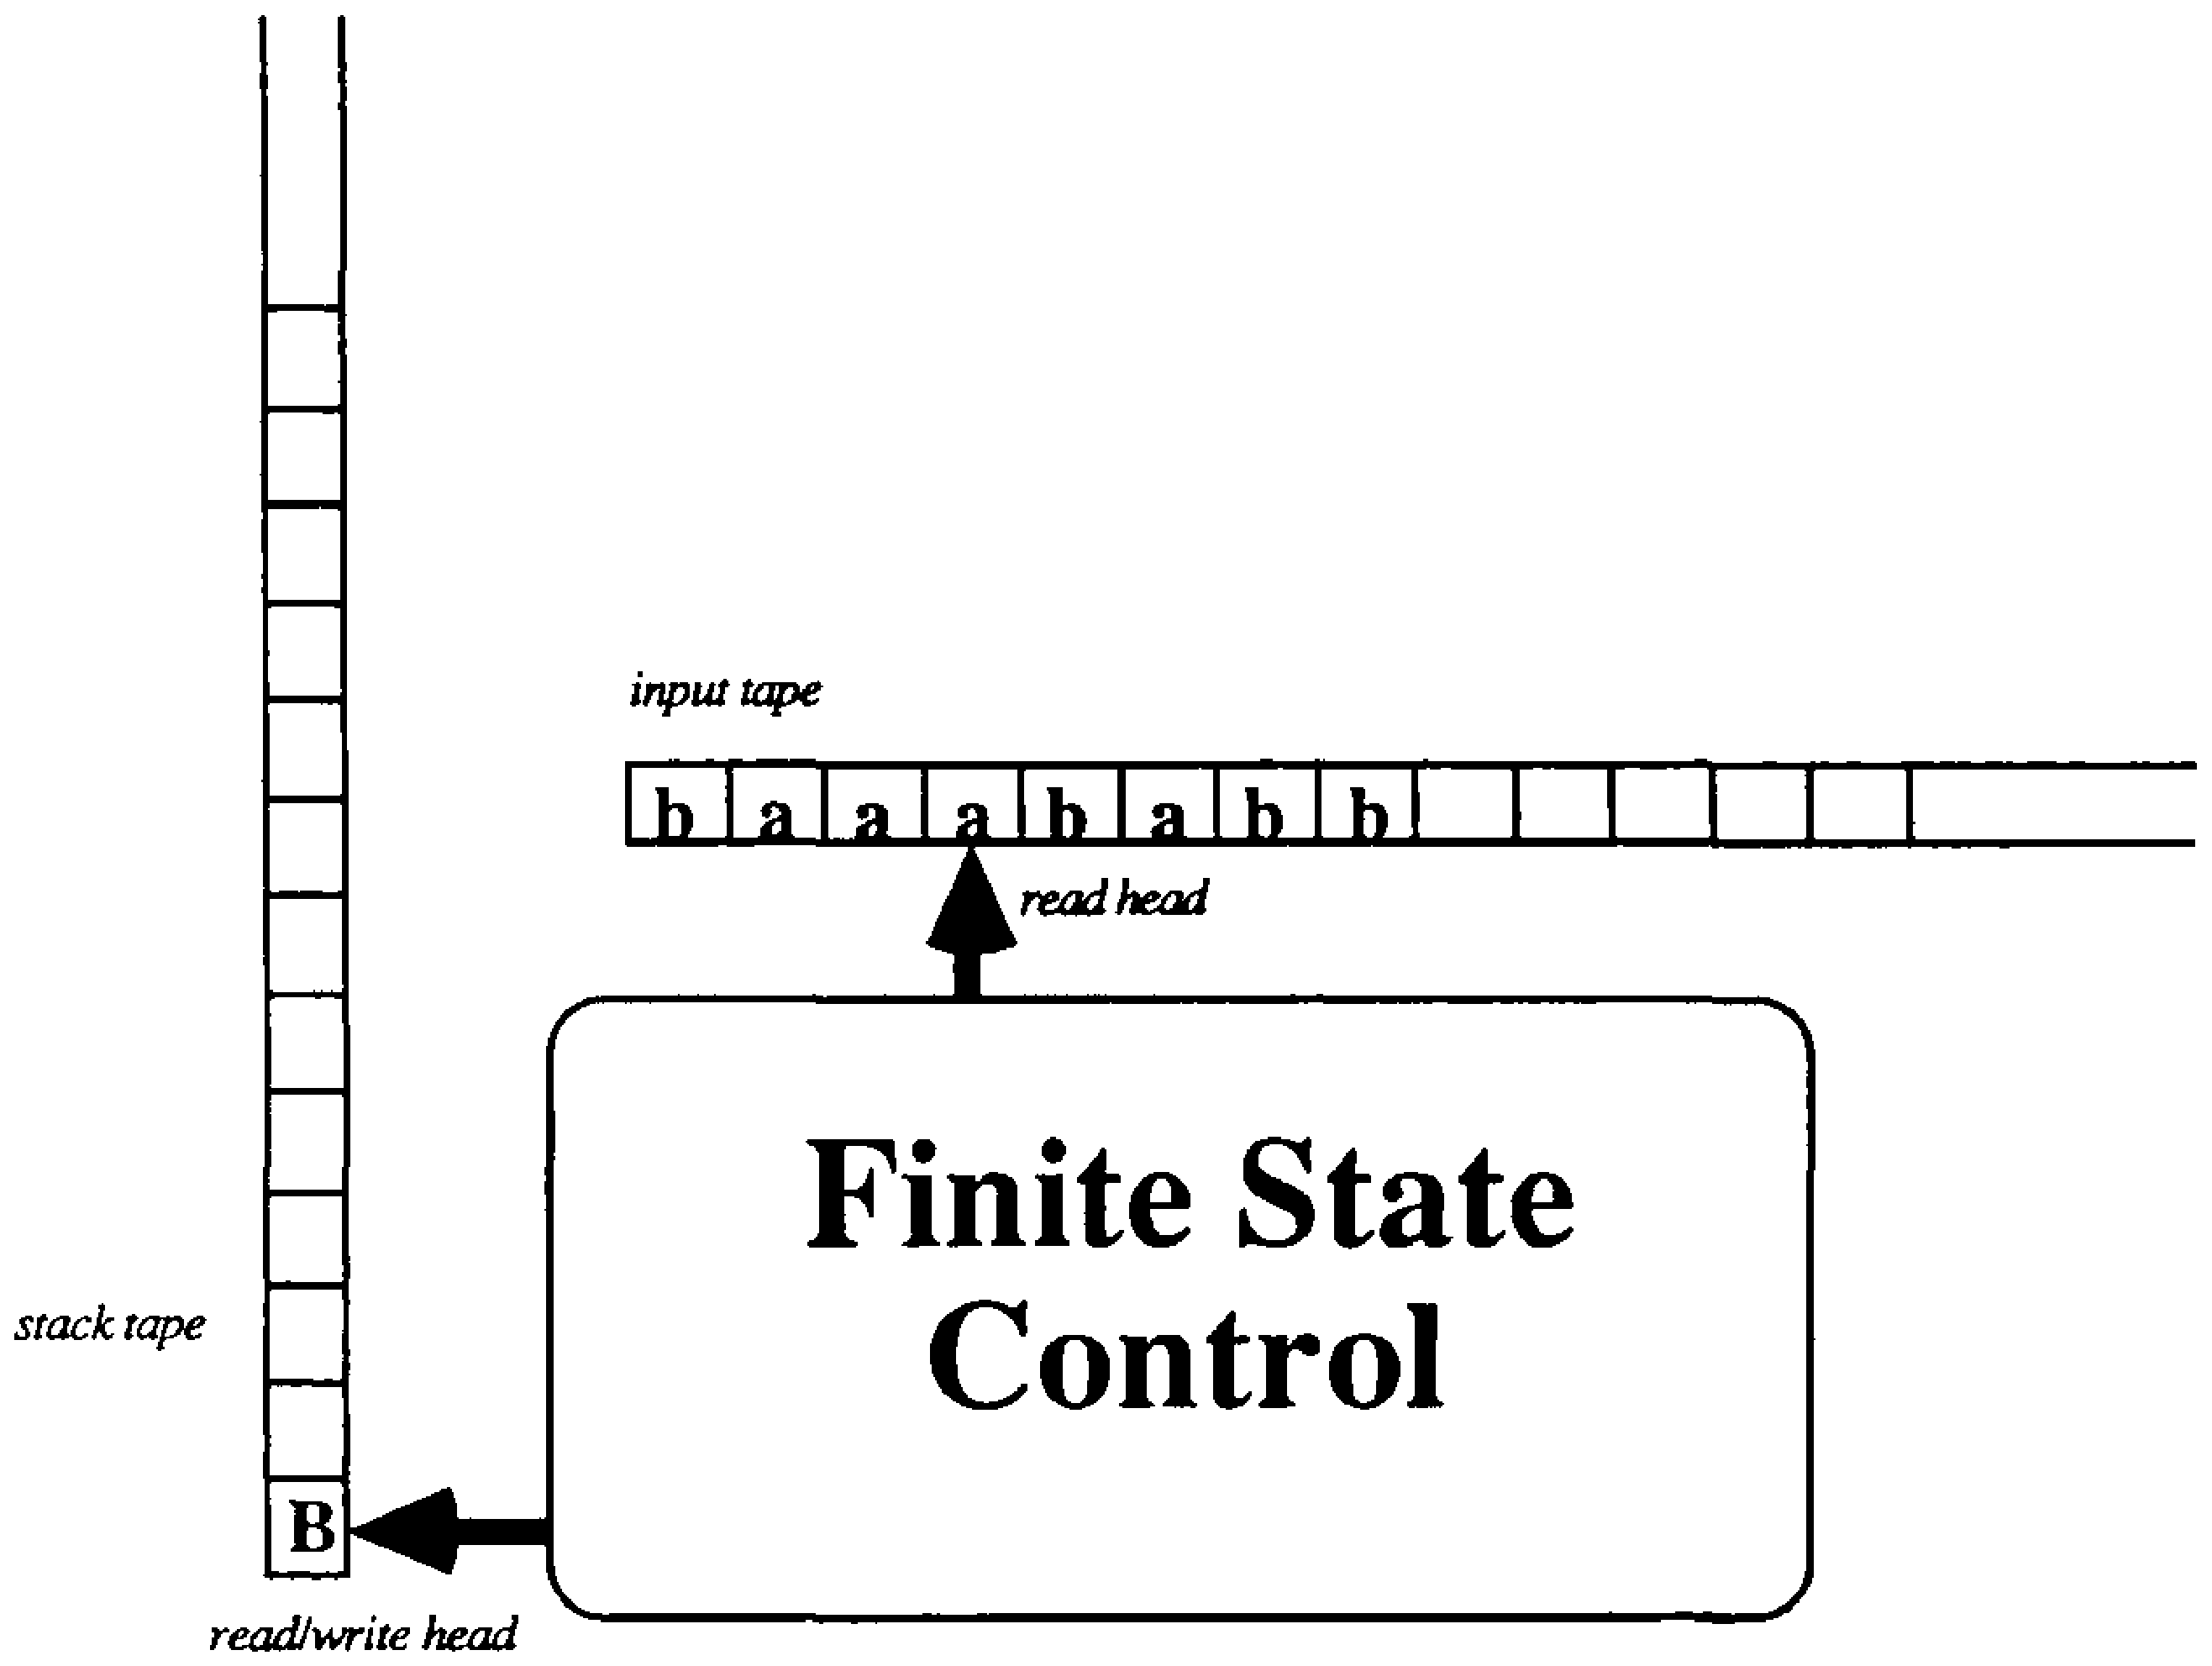
\epsfig{figure=ToFAfigures/fig10-1.eps,height=2.5in}}
\caption{A model of a pushdown automaton}\label{fig-10.1}
\end{figure}

The auxiliary tape\index{tape!auxiliary}\index{auxiliary tape of a PDA} is similar to that of a finite-state transducer; the second
component of the range of the state transition function in a pushdown automaton
specifies the string to be written on the stack tape. Thus, the functions
$\delta$ and $\omega$ of a FST are essentially combined in the $\delta$ function for
pushdown automata. The auxiliary tape differs from that of a FST in that the
current symbol from $\Gamma$ on the tape is sensed by the stack read/write head
and can affect the subsequent operation of the automaton. If no symbols are
written to tape during a transition, the tape head drops back one position and
will then be scanning the previous stack symbol. In essence, a state transition
is initiated by the currently scanned symbol on both the input tape and the
stack tape and begins with the stack symbol being popped from the stack; the
state transition is accompanied by a push operation, which writes a new string
of stack symbols on the stack tape. If several symbols are written, the
auxiliary read/write head will move ahead an appropriate amount, and the head
will be positioned over the last of the symbols written. Thus, if exactly one
symbol is written, the stack tape head does not move, and the effect is that the
old top-of-stack symbol is overwritten by the new symbol. When the empty string
is to be written, the effect is a pop followed by a push of no letters, and the
stack tape head retreats one position. If the only remaining stack symbol is
removed from the stack in this fashion, the stack tape head moves off the end
of the tape. It would then no longer be scanning a valid stack symbol, so no
further transitions are possible, and the device \emph{halts}.

It is possible to manipulate the stack and change states without consuming an
input letter, which is the intent of the $\lambda$-moves in the state transition
function. Since at most one symbol can be removed from the stack as a result of
a transition, $\lambda$-moves allow the stack to be shortened by several symbols
before the next input symbol is processed.

Acceptance can be defined by requiring the stack to be empty after the entire
input tape is consumed (as was the case with counting automata) or by requiring
that the automaton be in a final state after all the input is consumed. The
nondeterminism may allow the device to react to a given input string in several
distinct ways. As with NDFAs, the input word is considered accepted if at least
one of the possible reactions satisfies the criteria for acceptance. For a given
PDA, the set of words accepted by the empty stack criterion will likely differ
from the set of words accepted by the final state condition.

\subsection*{Example 10.1}

Consider the PDA defined by $P_1=\langle\{\pmb{a},\pmb{b}\},\{A,B\},\{q,r\},q,
\delta,B,\emptyset\rangle$, where $\delta$ is defined by
\begin{center}\begin{tabular}{r@{ = }l}
$\delta(q,\pmb{a},B)$ & $\{\langle q,A\rangle\}$ \\
$\delta(q,\pmb{a},A)$ & $\{\langle q,AA\rangle\}$ \\
$\delta(q,\pmb{b},B)$ & $\{\ \ \}$ \\
$\delta(q,\pmb{b},A)$ & $\{\langle r,\lambda\rangle\}$ \\
$\delta(r,\pmb{a},B)$ & $\{\ \ \}$ \\
$\delta(r,\pmb{a},A)$ & $\{\ \ \}$ \\
$\delta(r,\pmb{b},B)$ & $\{\ \ \}$ \\
$\delta(r,\pmb{b},A)$ & $\{\langle r,\lambda\rangle\}$
\end{tabular}\end{center}
Note that since the set of final states is empty no strings are accepted by
final state. We wish to consider the set of strings accepted by empty stack. In
general, when the set of final states is nonempty, the PDA will designate a
machine designed to accept by final state;\index{accept by final state} $F=\emptyset$ will generally be taken
as an indication that acceptance is to be by empty stack.\index{accept by empty stack}

The action of the state transition function can be displayed much like that of
finite-state transducers. Transition arrows are no longer labeled with just a
symbol from the input alphabet, since both a stack symbol and an input symbol
now govern the action of the automaton. Thus, arrows are labeled by ordered
pairs from $\Sigma\times\Gamma$. As with FSTs, this is followed by the output
caused by the transition. The diagram corresponding to $P_1$ is shown in Figure
\ref{fig-10.2}.

% Figure 10.2
\begin{figure}
\centerline{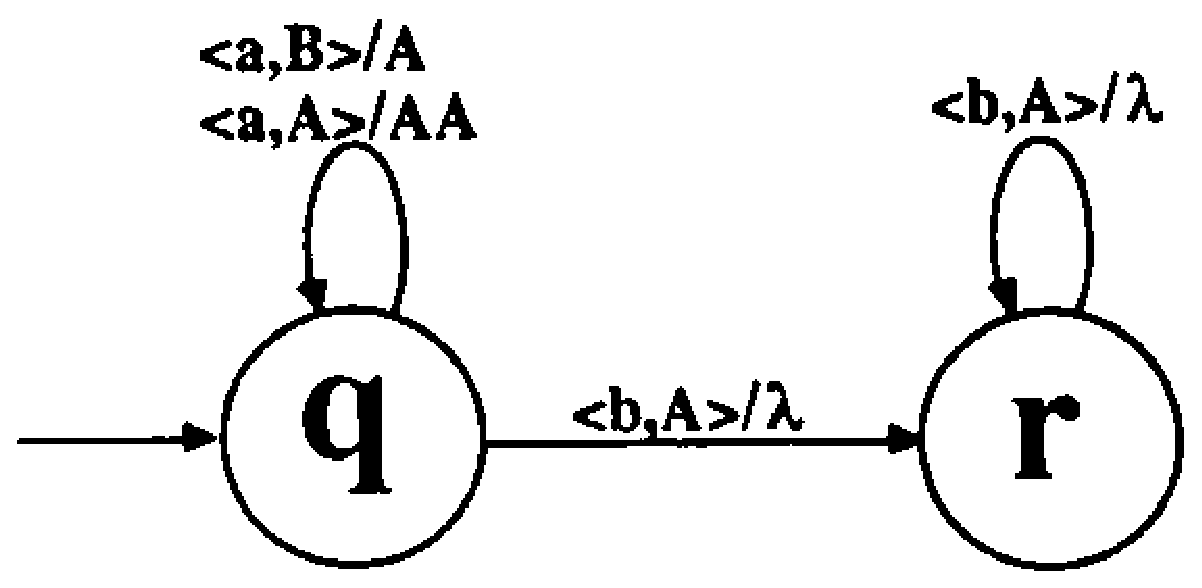
\epsfig{figure=ToFAfigures/fig10-2.eps,height=1in}}
\caption{The PDA discussed in Example 10.1}\label{fig-10.2}
\end{figure}

The reaction of $P_1$ to the string $\pmb{aabb}$ is the sequence of moves
displayed in Figures \ref{fig-10.3a}-e. Initially, the heads of the two tapes are positioned
as shown in Figure \ref{fig-10.3a}, with the (current) initial state highlighted. Since
the state is $q$, the input symbol is $\pmb{a}$, and the stack symbol is $B$, the
first transition rule $\delta(q,\pmb{a},B)=\{\langle q,A\rangle\}$ applies;
$P_1$ remains in state $q$, and the popped stack symbol $B$ is replaced by a
single $A$. Figure \ref{fig-10.3b} shows the new state of the automaton. The stack
read/write head is in the same position, since the length of the stack did not
change. The input read head moves on to the next letter, since the first input
symbol was consumed. The second rule now applies, and the single $A$ is replaced
by the pair $AA$ as $P_1$ returns to $q$ again, as shown in Figure \ref{fig-10.3c}. Note
that the stack tape head advanced as the topmost symbol was written. The rule
$\delta(q,\pmb{b},A)=\{\langle r,\lambda\rangle\}$ now applies, and the state
of the machine switches to $r$ as the (topmost) $A$ is popped and replaced with
an empty string, leaving the stack shorter than before. This is shown in Figure
\ref{fig-10.3d}. The last of the eight transition rules now applies, leaving the automaton
in the configuration shown by Figure \ref{fig-10.3e}. Since the stack is now empty, no
further moves are possible. However, since the read head has reached the end of
the input string, the word $\pmb{aabb}$ is accepted by $P_1$. The word $\pmb{aab}$
would be rejected by $P_1$ since the automaton would run out of input in a
configuration similar to that of Figure \ref{fig-10.3d}, in which the stack is not yet
empty. The word $\pmb{aabbb}$ would not be accepted because the stack would empty
prematurely, leaving $P_1$ stuck in a configuration similar to that of Figure
\ref{fig-10.3e}, but with the input string incompletely consumed. The word $\pmb{aaba}$
would likewise be rejected because there would be no move from the state $r$
with which to process the final input symbol $\pmb{a}$.

\setcounter{figure}{0}
\renewcommand{\thefigure}{\arabic{chapter}.3\alph{figure}}
% Figure 10.3a
\begin{figure}
\centerline{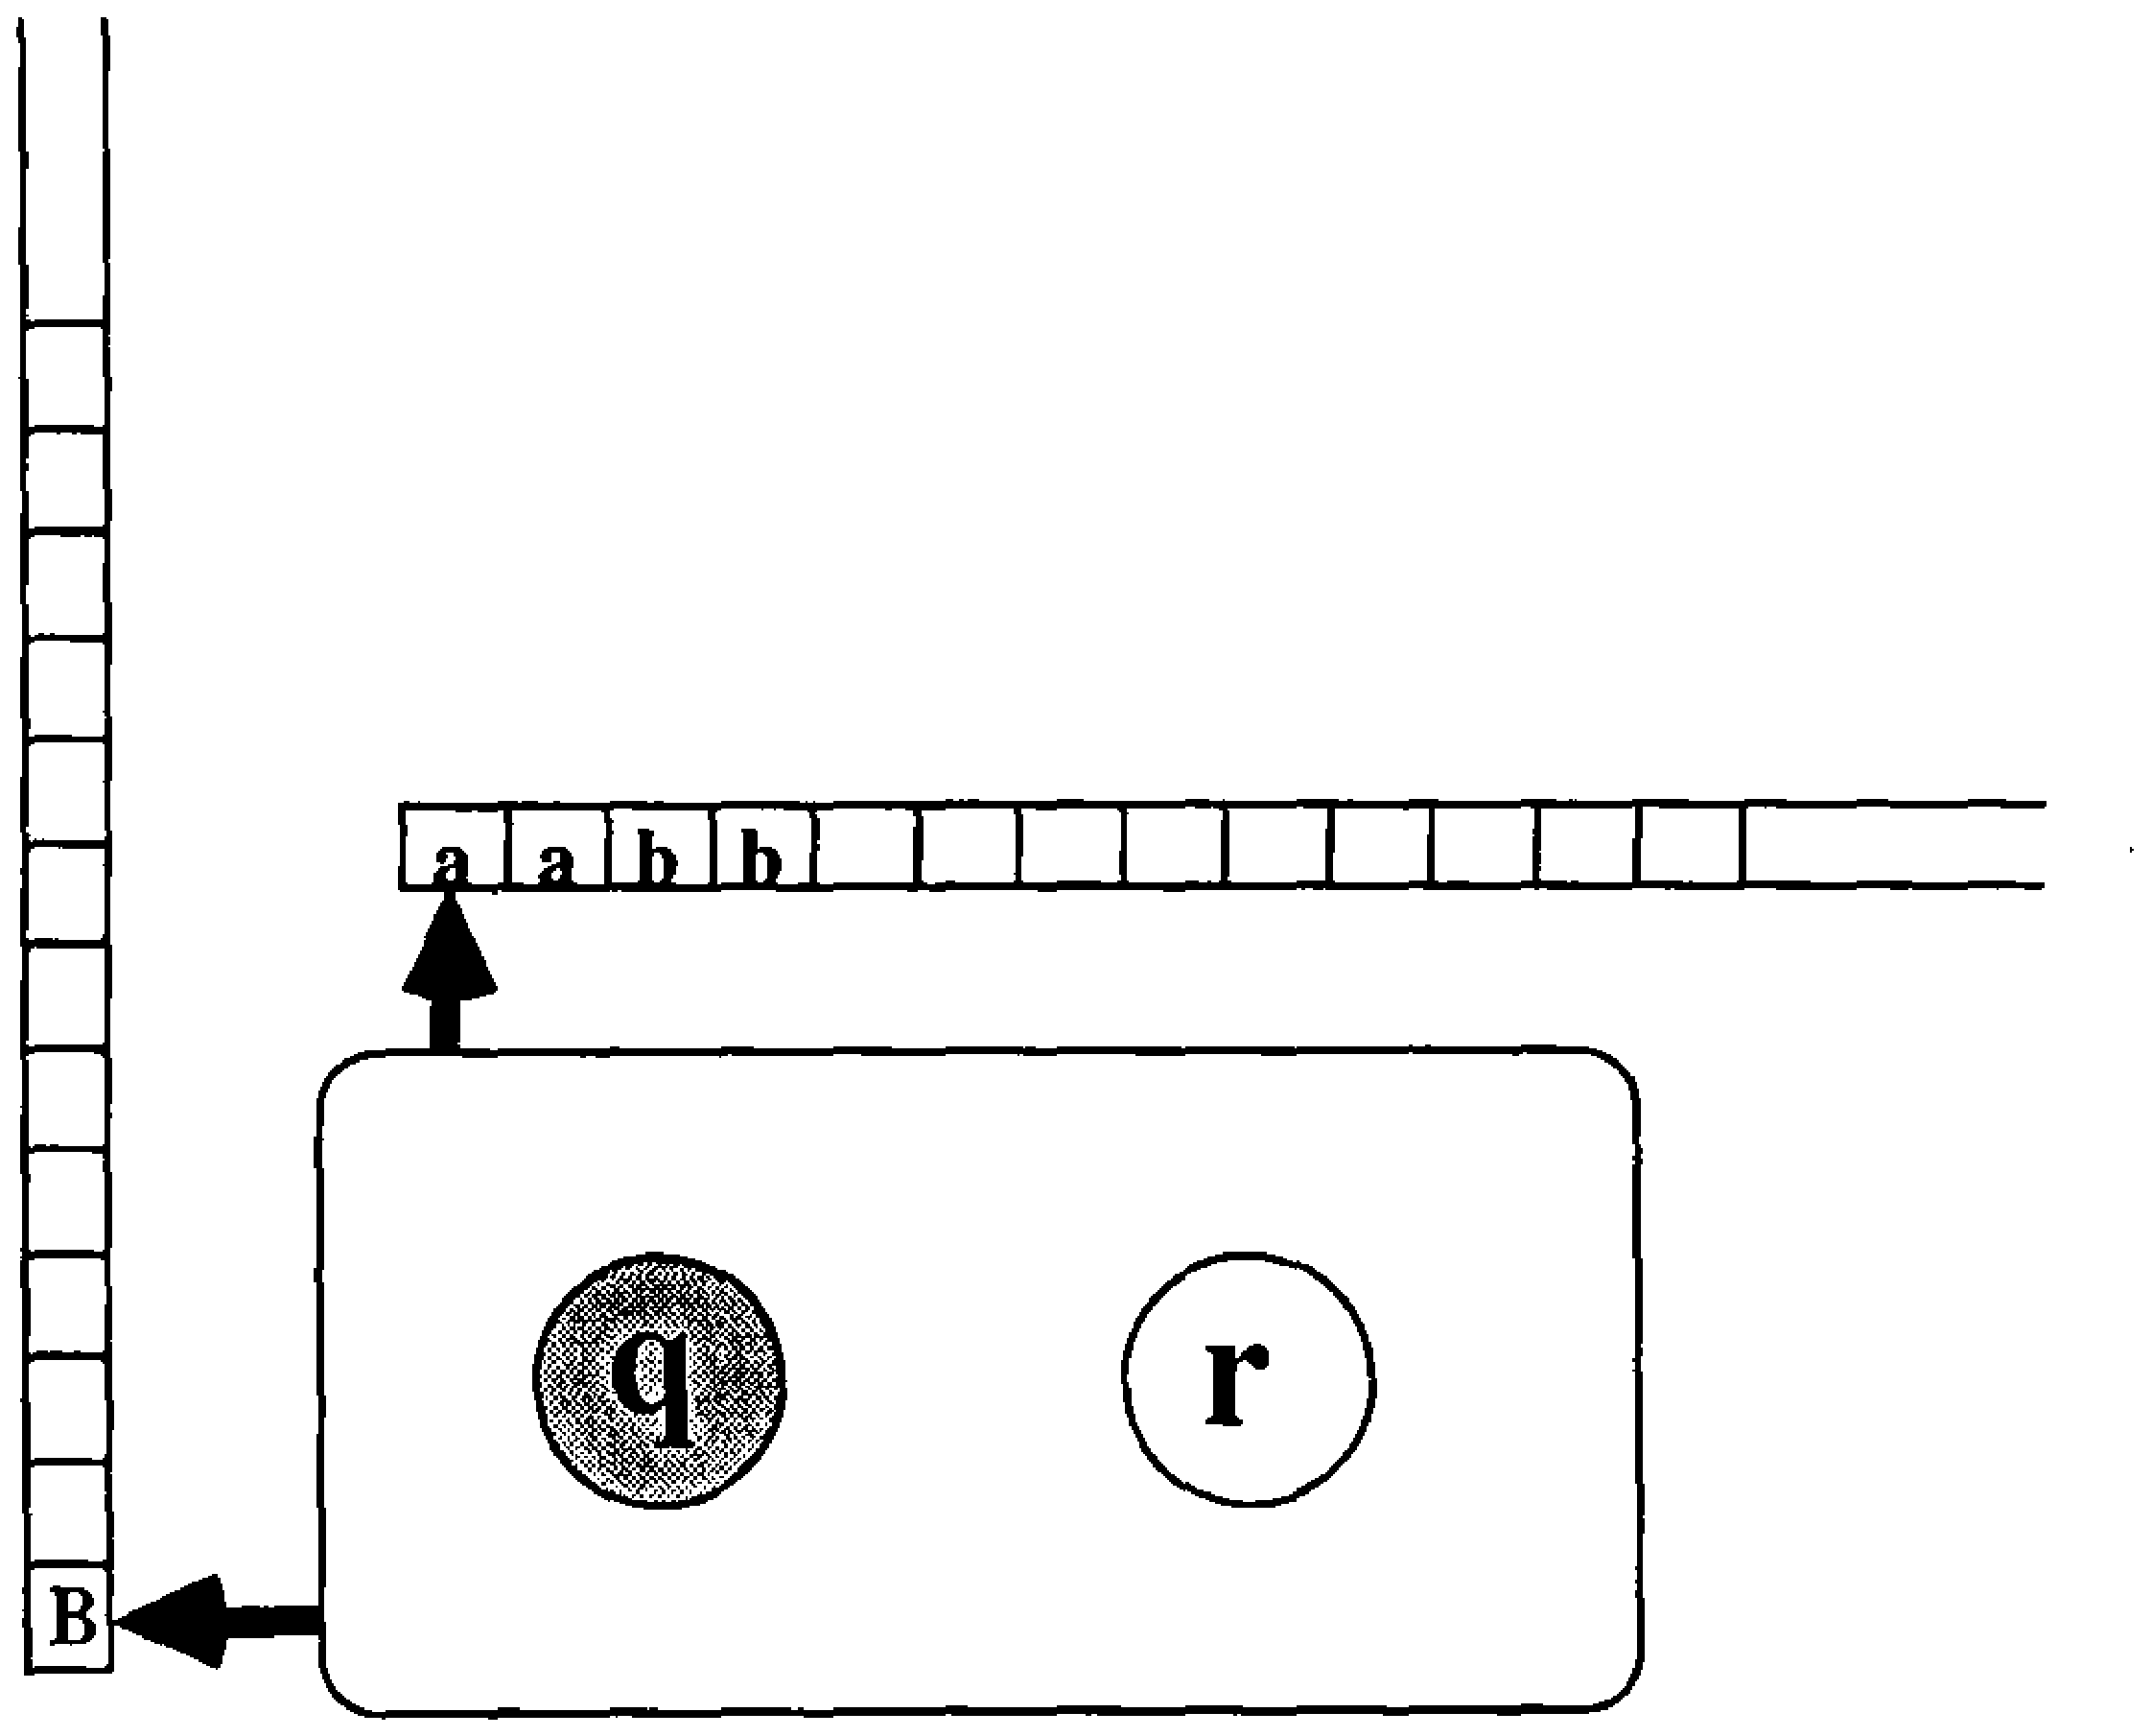
\epsfig{figure=ToFAfigures/fig10-3a.eps,height=2.0in}}
\caption{Walkthrough of the pushdown automaton discussed in Example 10.1}\label{fig-10.3a}
\end{figure}

% Figure 10.3b
\begin{figure}
\centerline{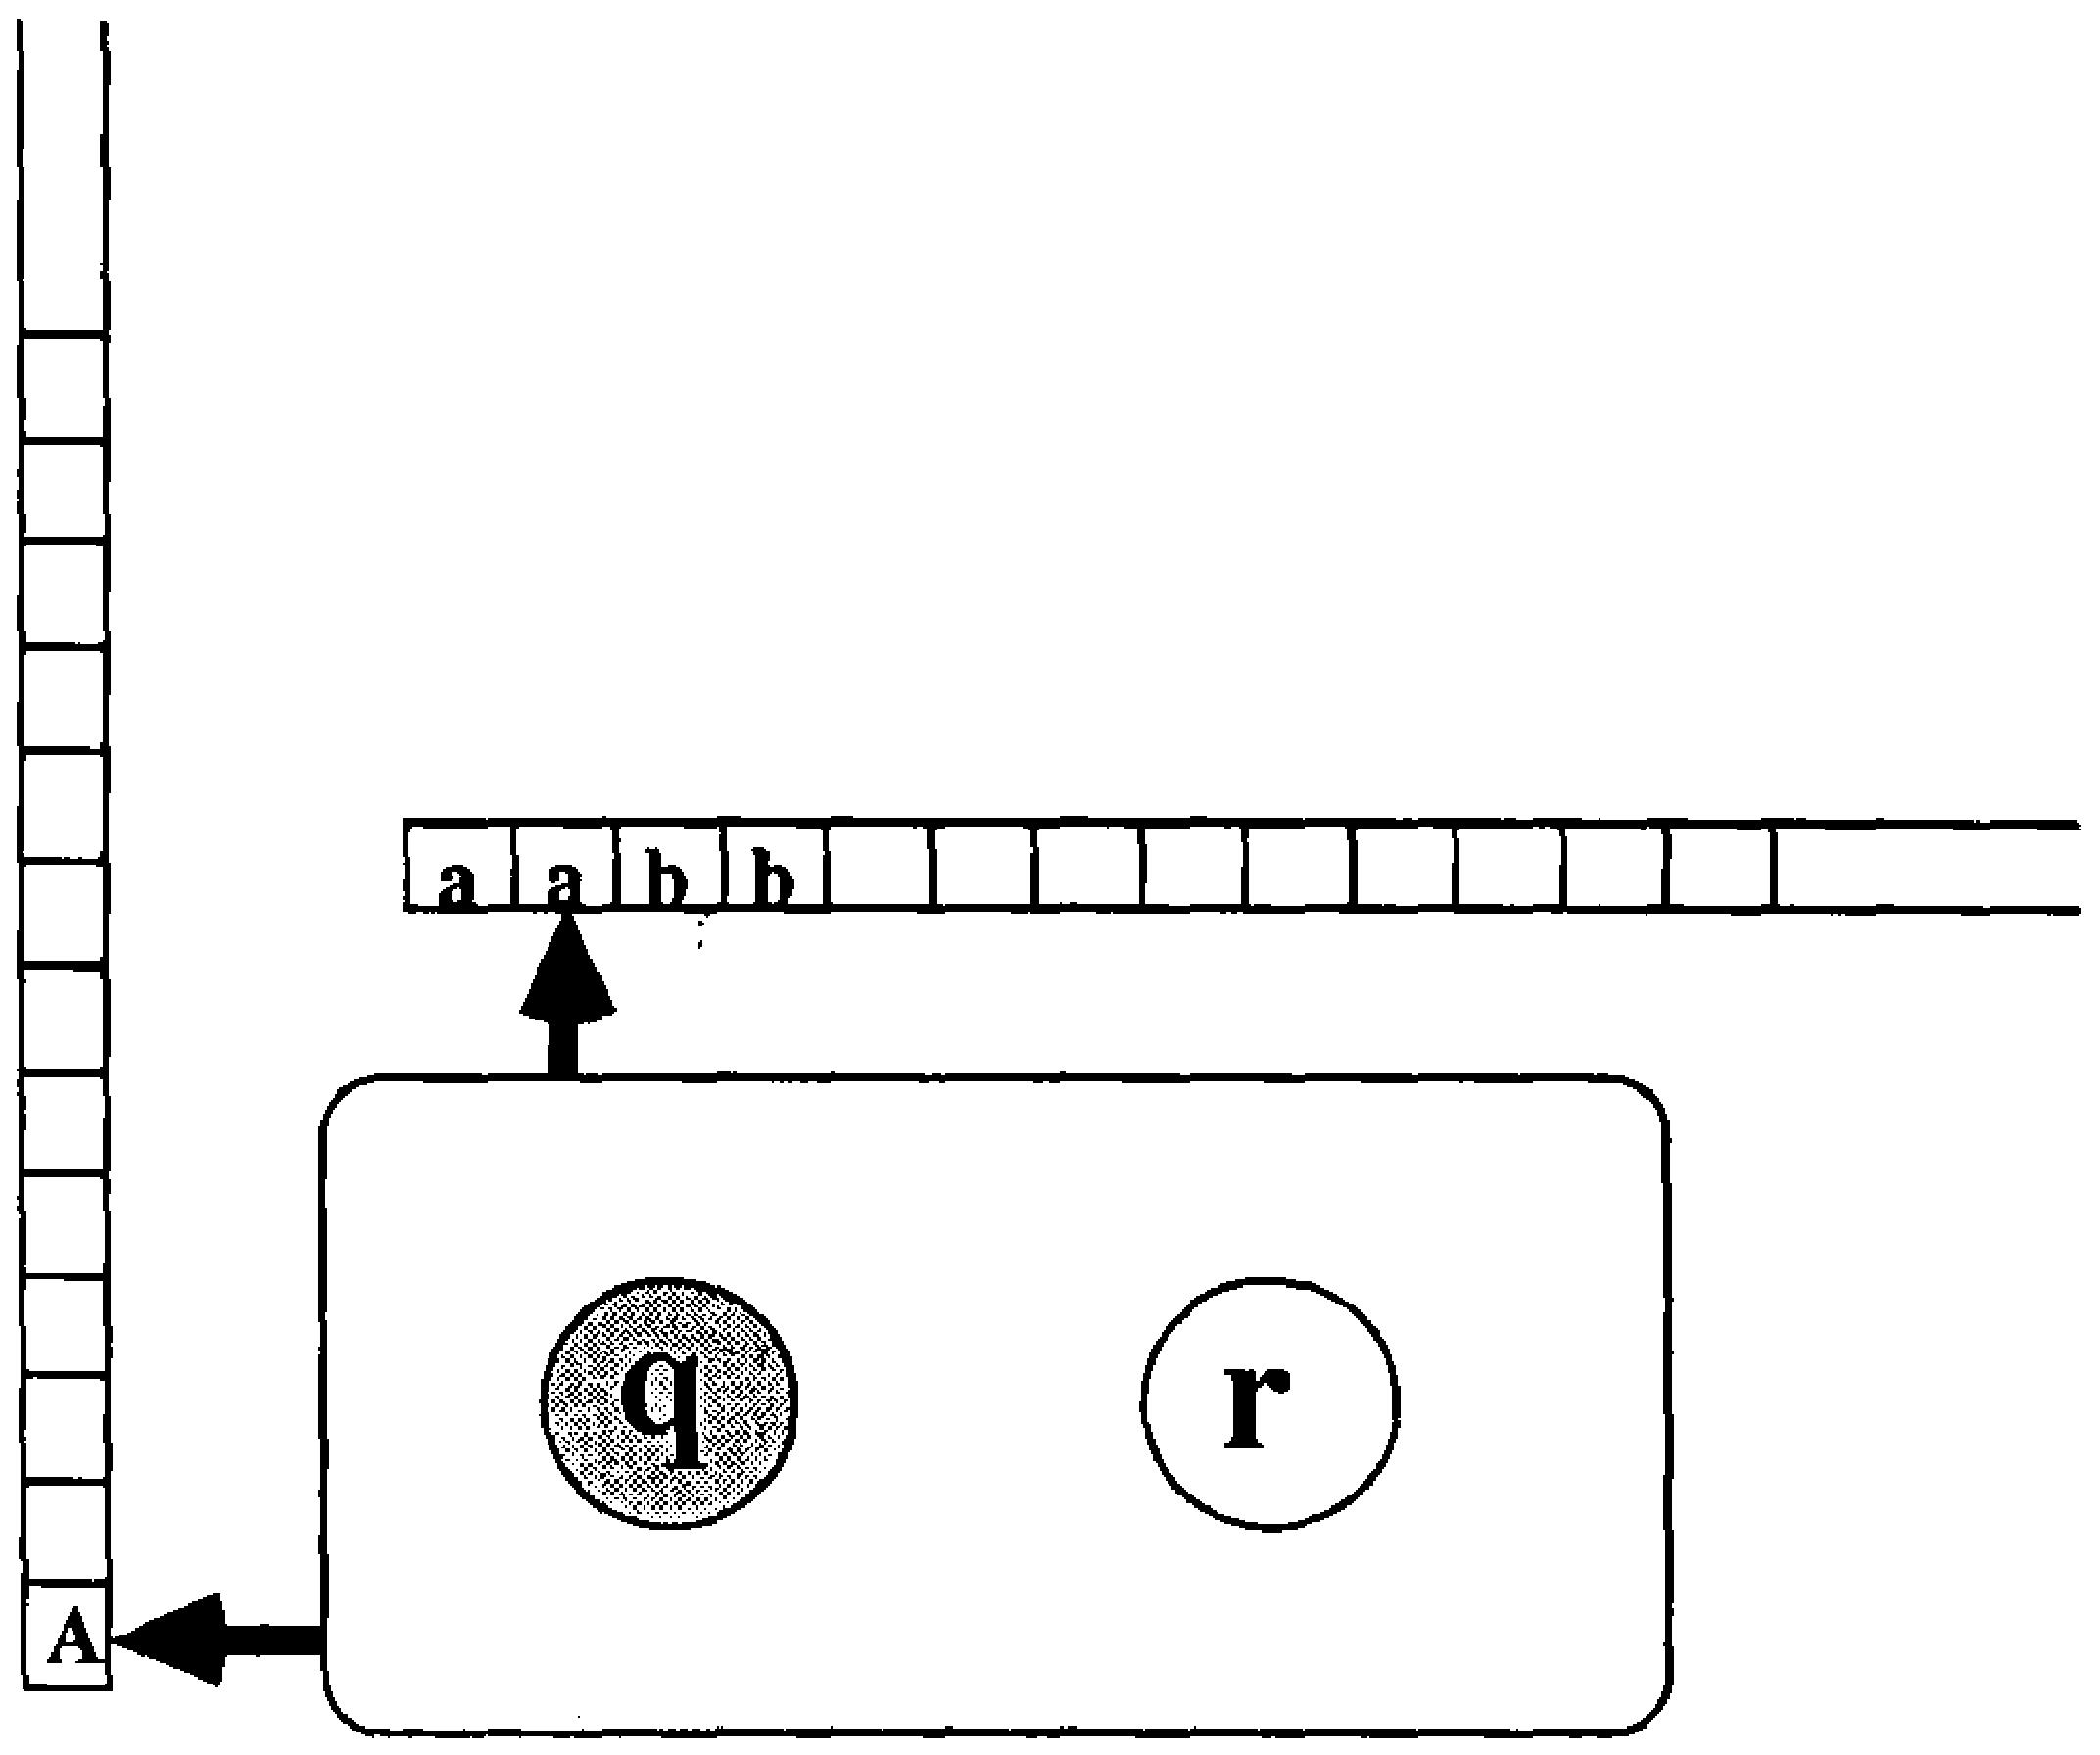
\epsfig{figure=ToFAfigures/fig10-3b.eps,height=2.0in}}
\caption{Walkthrough of the pushdown automaton discussed in Example 10.1}\label{fig-10.3b}
\end{figure}

% Figure 10.3c
\begin{figure}
\centerline{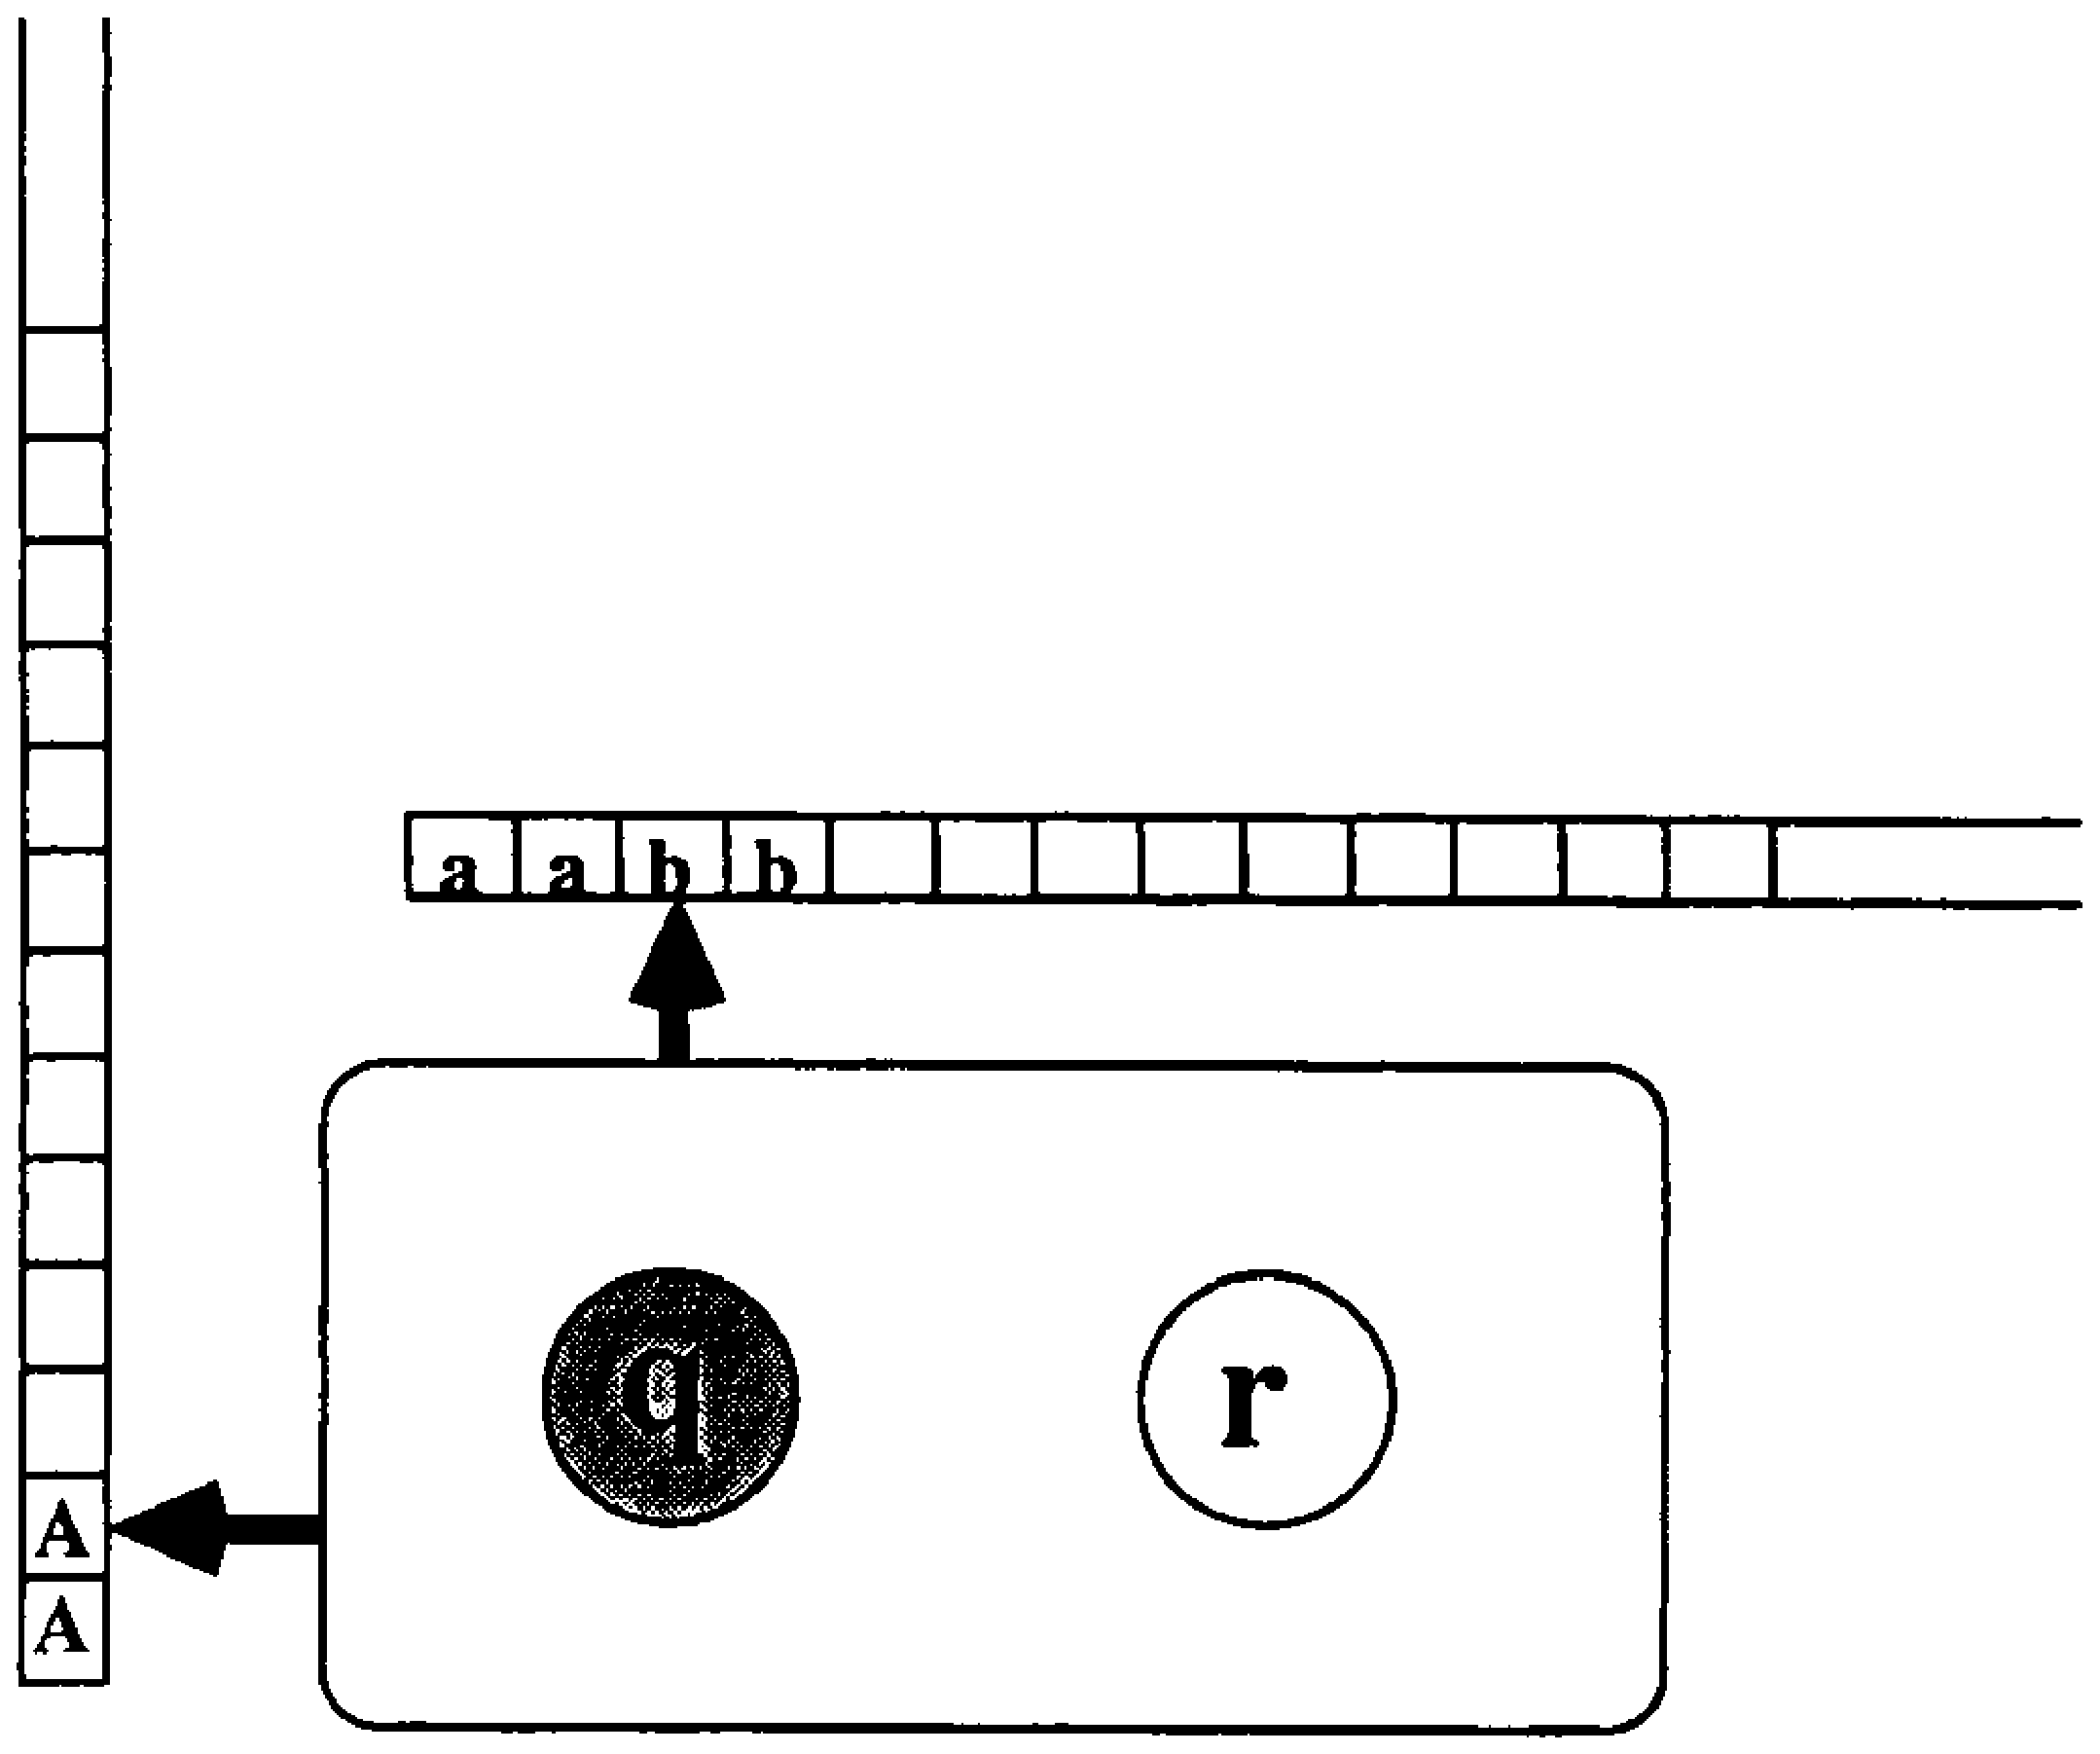
\epsfig{figure=ToFAfigures/fig10-3c.eps,height=2.0in}}
\caption{Walkthrough of the pushdown automaton discussed in Example 10.1}\label{fig-10.3c}
\end{figure}

% Figure 10.3d
\begin{figure}
\centerline{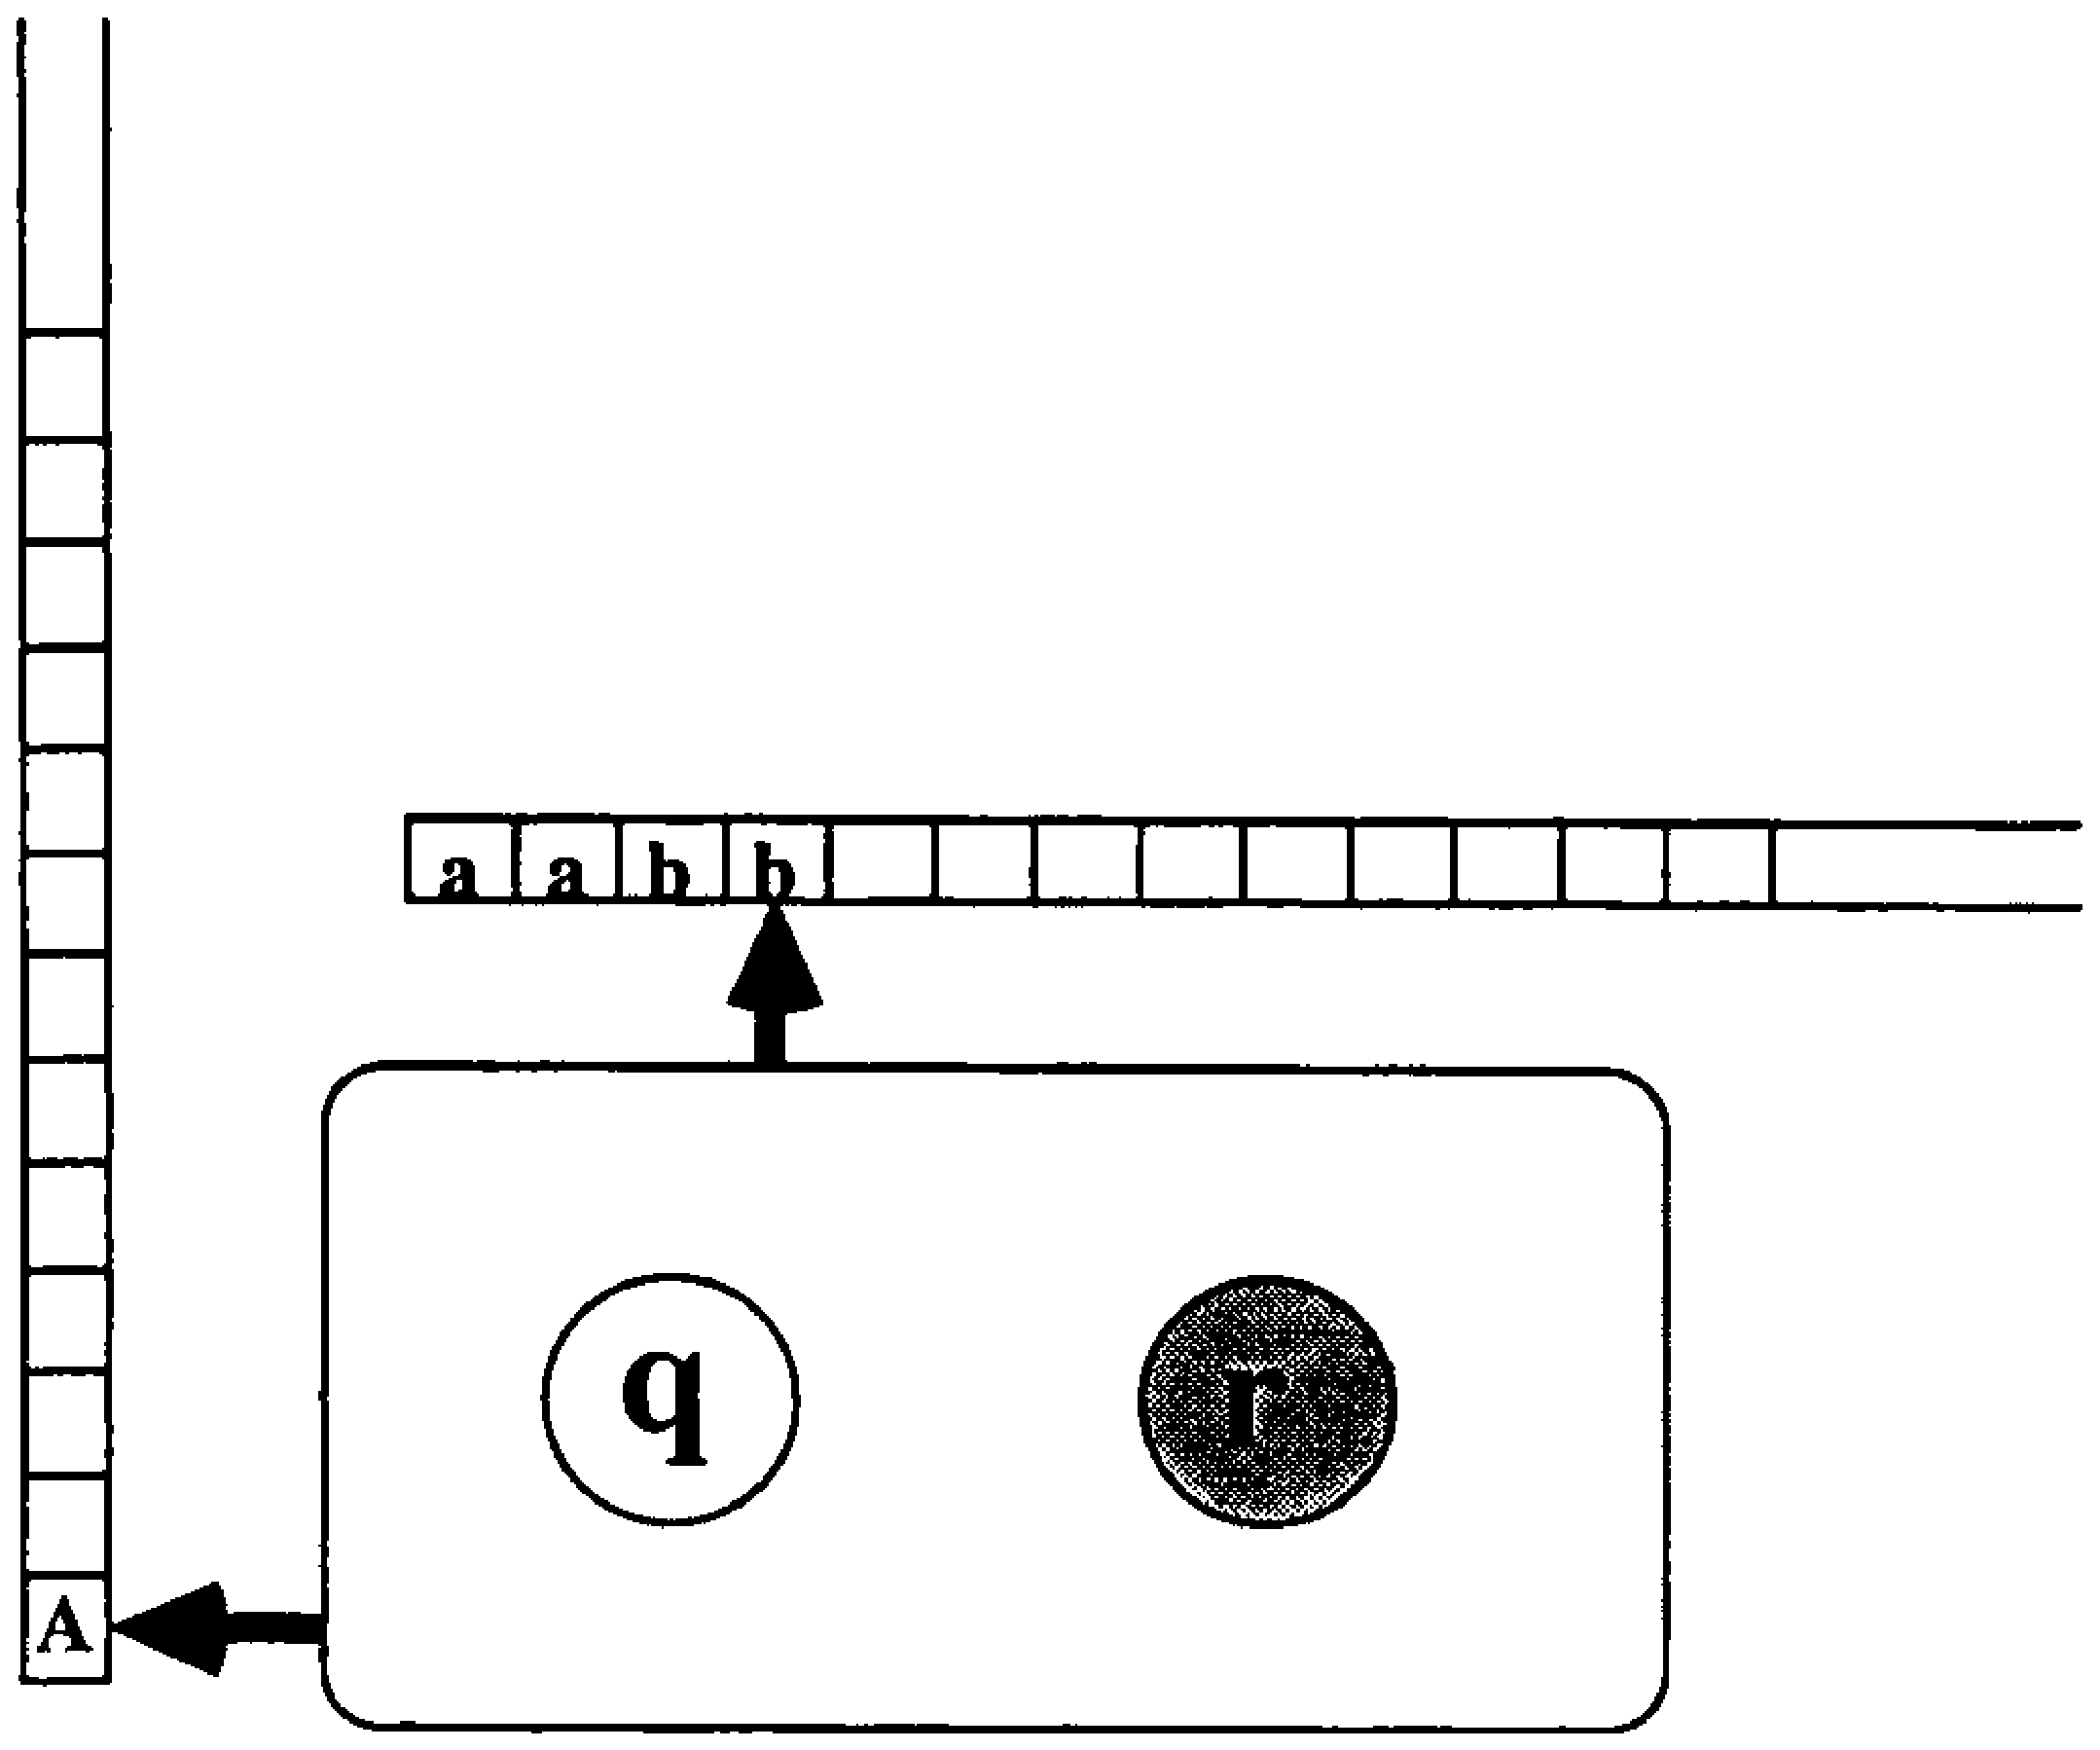
\epsfig{figure=ToFAfigures/fig10-3d.eps,height=2.0in}}
\caption{Walkthrough of the pushdown automaton discussed in Example 10.1}\label{fig-10.3d}
\end{figure}

% Figure 10.3e
\begin{figure}
\centerline{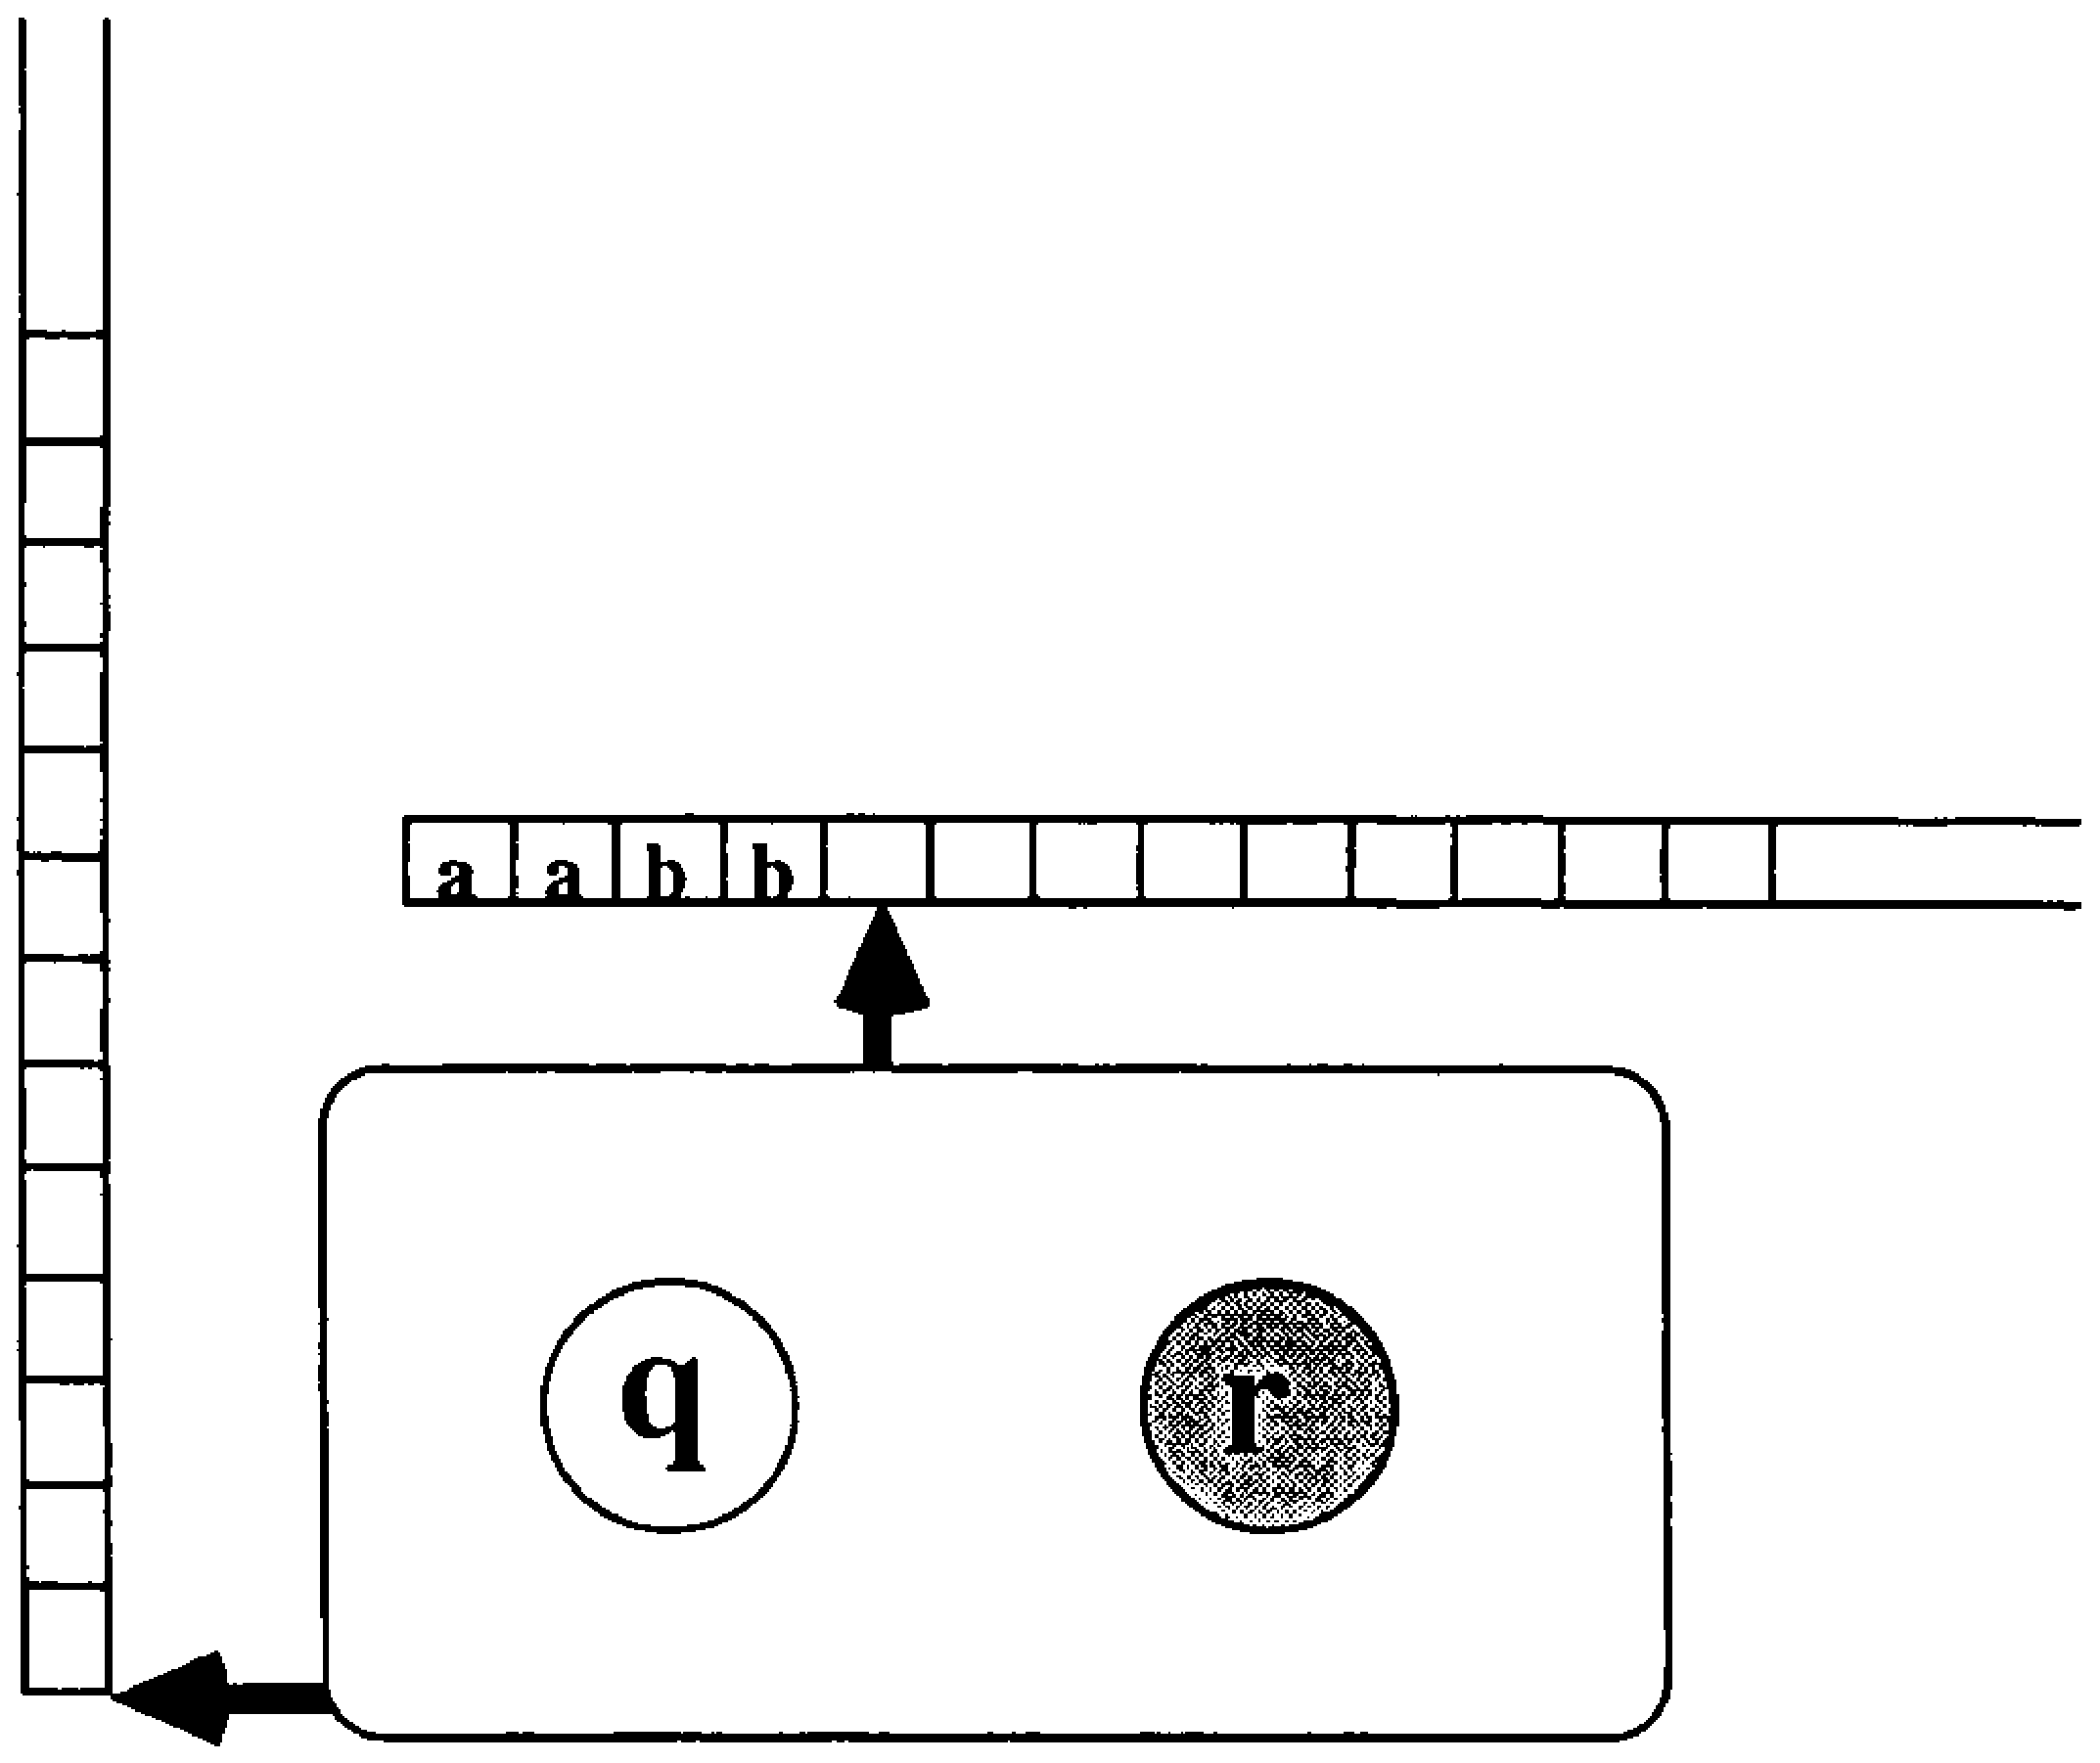
\epsfig{figure=ToFAfigures/fig10-3e.eps,height=2.0in}}
\caption{Walkthrough of the pushdown automaton discussed in Example 10.1}\label{fig-10.3e}
\end{figure}
\setcounter{figure}{3} %nasty kluge: latex thinks it's now up to figure 8, not 4
\renewcommand{\thefigure}{\arabic{chapter}.\arabic{figure}}

As with deterministic finite automata, once an input symbol is consumed, it has
no further effect on the operation of the pushdown automaton. The current state
of the device, the remaining input symbols, and the current stack contents form
a triple that describes the current configuration of the PDA. The triple
$\langle q,\pmb{bb},AA\rangle$ thus describes the configuration of the PDA in Figure
\ref{fig-10.3c}. When processing $\pmb{aabb}$, $P_1$ moved through the following sequence of
configurations:

\begin{center}\begin{tabular}{l}
$\langle q,\pmb{aabb},B\rangle$ \\
$\langle q,\pmb{abb},A\rangle$ \\
$\langle q,\pmb{bb},AA\rangle$ \\
$\langle r,\pmb{b},A\rangle$ \\
$\langle r,\lambda,\lambda\rangle$
\end{tabular}\end{center}
Successive configurations followed from their predecessors by applying a single
rule from the state transition function. These transitions will be described by
the operator $\vdash$.

% Definition 10.2
\begin{dfn}\label{dfn-10.2}
The current \emph{configuration} of pushdown automaton $P=\langle\Sigma,\Gamma,
S,s_0,\delta,B,F\rangle$ is described by a triple $\langle s,x,\alpha\rangle$,
where
\begin{quote}
$s$ is the current state. \\
$x$ is the unconsumed portion of the input string. \\
$\alpha$ is the current stack contents (with the topmost symbol written as the
leftmost).
\end{quote}

An ordered pair $\langle t,\gamma\rangle$ within the finite set of objects specified by
$\delta(s,\pmb{a},A)$ can cause a \emph{move} in the pushdown automaton $P$ from
the configuration $\langle s,\pmb{a}y,A\beta\rangle$ to the configuration $\langle t,y,\gamma\beta\rangle$.
This transition is denoted as $\langle s,\pmb{a}y,A\beta\rangle\vdash\langle t,y,\gamma\beta\rangle$.

A sequence of successive moves in which
\[ \langle s_1,x_1,\alpha_1\rangle\vdash\langle s_2,x_2,\alpha_2\rangle,\langle
	s_2,x_2,\alpha_2\rangle\vdash\langle s_3,x_3,\alpha_3\rangle,\ldots,
	\langle s_{m-1},x_{m-1},\alpha_{m-1}\rangle\vdash\langle s_m,x_m,
	\alpha_m\rangle \]
is denoted by $\langle s_1,x_1,\alpha_1\rangle\Dvdash\langle s_m,x_m,\alpha_m\rangle$.
\end{dfn}
The operator\ $\Dvdash$\ reflects the reflexive and transitive closure of $\vdash$,
and thus we also have $\langle s_1,x_1,\alpha_1\rangle\Dvdash\langle s_1,x_1,\alpha_1\rangle$ and clearly
$\langle s_1,x_1,\alpha_1\rangle\vdash\langle s_2,x_2,\alpha_2\rangle$ implies $\langle s_1,x_1,\alpha_1\rangle\Dvdash
\langle s_2,x_2,\alpha_2\rangle$.

\subsection*{Example 10.2}

For the pushdown automaton $P_1$ in Example 10.1, $\langle q,\pmb{aabb},B\rangle
\Dvdash\langle r,\lambda,\lambda\rangle$ because $\langle q,\pmb{aabb},B\rangle
\vdash\langle q,\pmb{abb},A\rangle\vdash\langle q,\pmb{bb},AA\rangle\vdash
\langle r,\pmb{b},A\rangle\vdash\langle r,\lambda,\lambda\rangle$.

% Definition 10.3
\begin{dfn}\label{dfn-10.3}\index{language!accepted by final state PDA}\index{language!accepted by empty stack PDA}
For a pushdown automaton $P=\langle\Sigma,\Gamma,S,s_0,\delta,B,F\rangle$, the
\emph{language accepted via final state} by $P$, $L(P)$, is
\[ \{x\in\Sigma^*|\ \exists r\in F,\exists\alpha\in\Gamma^*\ni\langle s_0,x,B
	\rangle\Dvdash\langle r,\lambda,\alpha\rangle\} \]
\emph{The language accepted via empty stack} by $P$, $\Lambda(P)$, is
\[ \{x\in\Sigma^*|\ \exists r\in S\ni\langle s_0,x,B\rangle\Dvdash\langle r,
	\lambda,\lambda\rangle\} \]
\end{dfn}

\subsection*{Example 10.3}

Consider the pushdown automaton $P_1$ in Example 10.1. Since only strings of the
form $\pmb{a}^i\pmb{b}^i$ (for $i \geq 1$) allow $\langle q,\pmb{a}^i\pmb{b}^i,
B\rangle\Dvdash\langle r,\lambda,\lambda\rangle$, it follows that $\Lambda(P_1)
=\{\pmb{a}^n\pmb{b}^n|\ n\geq 1\}$. However, $F=\emptyset$ and thus $L(P_1$) is
clearly $\emptyset$.

The pushdown automaton $P_1$ in Example 10.1 was \emph{deterministic} in the
sense that there will never be more than one choice that can be made from any
configuration. The following example illustrates a pushdown automaton that is
nondeterministic.

\subsection*{Example 10.4}

Consider the pushdown automaton defined by $P_2=\langle\{\pmb{a},\pmb{b}\},\{S,
C\},\{t\},t,\delta,S,\emptyset\rangle$, where $\delta$ is defined by
\begin{center}\begin{tabular}{r@{ = }l}
$\delta(t,\pmb{a},S)$ & $\{\langle t,SC\rangle,\langle t,C\rangle\}$ \\
$\delta(t,\pmb{a},C)$ & $\{\ \ \}$ \\
$\delta(t,\pmb{b},S)$ & $\{\ \ \}$ \\
$\delta(t,\pmb{b},C)$ & $\{\langle t,\lambda\rangle\}$ \\
$\delta(t,\lambda,S)$ & $\{\ \ \}$ \\
$\delta(t,\lambda,C)$ & $\{\ \ \}$
\end{tabular}\end{center}
In this automaton, there are two distinct courses of action when the input
symbol is $\pmb{a}$ and the top stack symbol is $S$, which leads to several
possible options when trying to process the word $\pmb{aabb}$. One option is to
apply the first move whenever possible, which leads to the sequence of
configurations
\[ \langle t,\pmb{aabb},S\rangle\vdash\langle t,\pmb{abb},SC\rangle\vdash\langle
	t,\pmb{bb},SCC\rangle. \]
Since there are no $\lambda$-moves and $\delta(t,\pmb{b},S)=\{\ \ \}$, there are
no further moves that can be made, and the input word cannot be completely
consumed in this manner. Another option is to choose the second move option
exclusively, leading to the abortive sequence $\langle t,\pmb{aabb},S\rangle
\vdash\langle t,\pmb{abb},C\rangle$; $\delta(t,\pmb{a},C)=\{\ \ \}$, and
processing again cannot be completed. A mixture of the first and second moves
results in the sequence $\langle t,\pmb{aabb},S\rangle\vdash\langle t,\pmb{abb},
SC\rangle\vdash\langle t,\pmb{bb},CC\rangle\vdash\langle t,\pmb{b},C\rangle
\vdash\langle t,\lambda,\lambda\rangle$, and $\pmb{aabb}$ is thus accepted by
$P_2$. Further experimentation shows that $\Lambda(P_2)=\{\pmb{a}^n\pmb{b}^n|\ n
\geq 1\}$. To successfully empty its stack, this automaton must correctly
``guess'' when the last $\pmb{a}$ is being read and choose the second transition
pair, placing only $C$ on the stack.

% Definition 10.4
\begin{dfn}\label{dfn-10.4}\index{equivalent!PDAs}
Two pushdown automata $M_1=\langle\Sigma,\Gamma_1,S_1,s_{0_1},\delta_1,B_1,F_1
\rangle$ and $M_2=\langle\Sigma,\Gamma_2,S_2,s_{0_2},\delta_2,\\ B_2,F_2\rangle$
are called \emph{equivalent} iff they accept the same language.
\end{dfn}

The pushdown automaton $P_1$ from Example 10.1 is therefore equivalent to $P_2$
in Example 10.4. The concept of equivalence will apply even if one device
accepts via final state and the other accepts via empty stack. In keeping with
the previous broad use of the concept of equivalence, if any two finite
descriptors define the same language, those descriptors will be called
equivalent. Thus, if a PDA $M$ happens to accept the language described by a
regular expression $R$, we will say that $R$ is equivalent to $M$.

\subsection*{Example 10.5}

The following pushdown automaton illustrates the use of $\lambda$-moves and
acceptance by final state for the language $\{\pmb{a}^n\pmb{b}^m|\ n\geq 1\wedge
(n=m \vee n=2m)\}$. Let $P_3=\langle\{\pmb{a},\pmb{b}\},\{A\},\{s_0\},\{s_0,s_1,
s_2,s_3,s_4\},\delta,A,\{s_2,s_4\}\rangle$, where $\delta$ is defined by
\begin{center}\begin{tabular}{r@{ = }l}
$\delta(s_0,\pmb{a},A)$ & $\{\langle s_0,AA\rangle\}$ \\
$\delta(s_0,\pmb{b},A)$ & $\{\ \ \}$ \\
$\delta(s_0,\lambda,A)$ & $\{\langle s_1,\lambda\rangle,\langle s_3,\lambda
	\rangle\}$ \\
$\delta(s_1,\pmb{a},A)$ & $\{\ \ \}$ \\
$\delta(s_1,\pmb{b},A)$ & $\{\langle s_1,\lambda\rangle\}$ \\
$\delta(s_1,\lambda,A)$ & $\{\langle s_2,\lambda\rangle\}$ \\
$\delta(s_2,\pmb{a},A)$ & $\{\ \ \}$ \\
$\delta(s_2,\pmb{b},A)$ & $\{\ \ \}$ \\
$\delta(s_2,\lambda,A)$ & $\{\ \ \}$ \\
$\delta(s_3,\pmb{a},A)$ & $\{\ \ \}$ \\
$\delta(s_3,\pmb{b},A)$ & $\{\ \ \}$ \\
$\delta(s_3,\lambda,A)$ & $\{\langle s_4,\lambda\rangle\}$ \\
$\delta(s_4,\pmb{a},A)$ & $\{\ \ \}$ \\
$\delta(s_4,\pmb{b},A)$ & $\{\langle s_3,\lambda\rangle\}$ \\
$\delta(s_4,\lambda,A)$ & $\{\ \ \}$
\end{tabular}\end{center}
The finite-state control for this automaton is diagrammed in Figure \ref{fig-10.4}. Note
that the $\lambda$-move from state $s_3$ is \emph{not} responsible for any
nondeterminism in this machine. From $s_3$, only one move is permissible: the
$\lambda$-move to $s_4$. On the other hand, the $\lambda$-move from state $s_1$
does allow a choice of moving to $s_2$ (without moving the read head) or staying
at $s_1$ while consuming another input symbol. The choice of moves from state
$s_0$ also contributes to the nondeterminism; the device must ``guess'' whether
the number of $\pmb{b}$s will equal the number of $\pmb{a}$s or whether there will
be half as many, and at the appropriate time transfer control to $s_1$ or $s_3$,
respectively. Notice that the moves defined by states $s_3$ and $s_4$ allow
\emph{two} stack symbols to be removed for each $\pmb{b}$ consumed. Furthermore, a
string like $\pmb{aab}$ can transfer control to $s_3$ as the final $\pmb{b}$ is
processed, but the $\lambda$-move can then be applied to reach $s_4$ even though
there are no more symbols on the input tape.

% Figure 10.4
\begin{figure}
\centerline{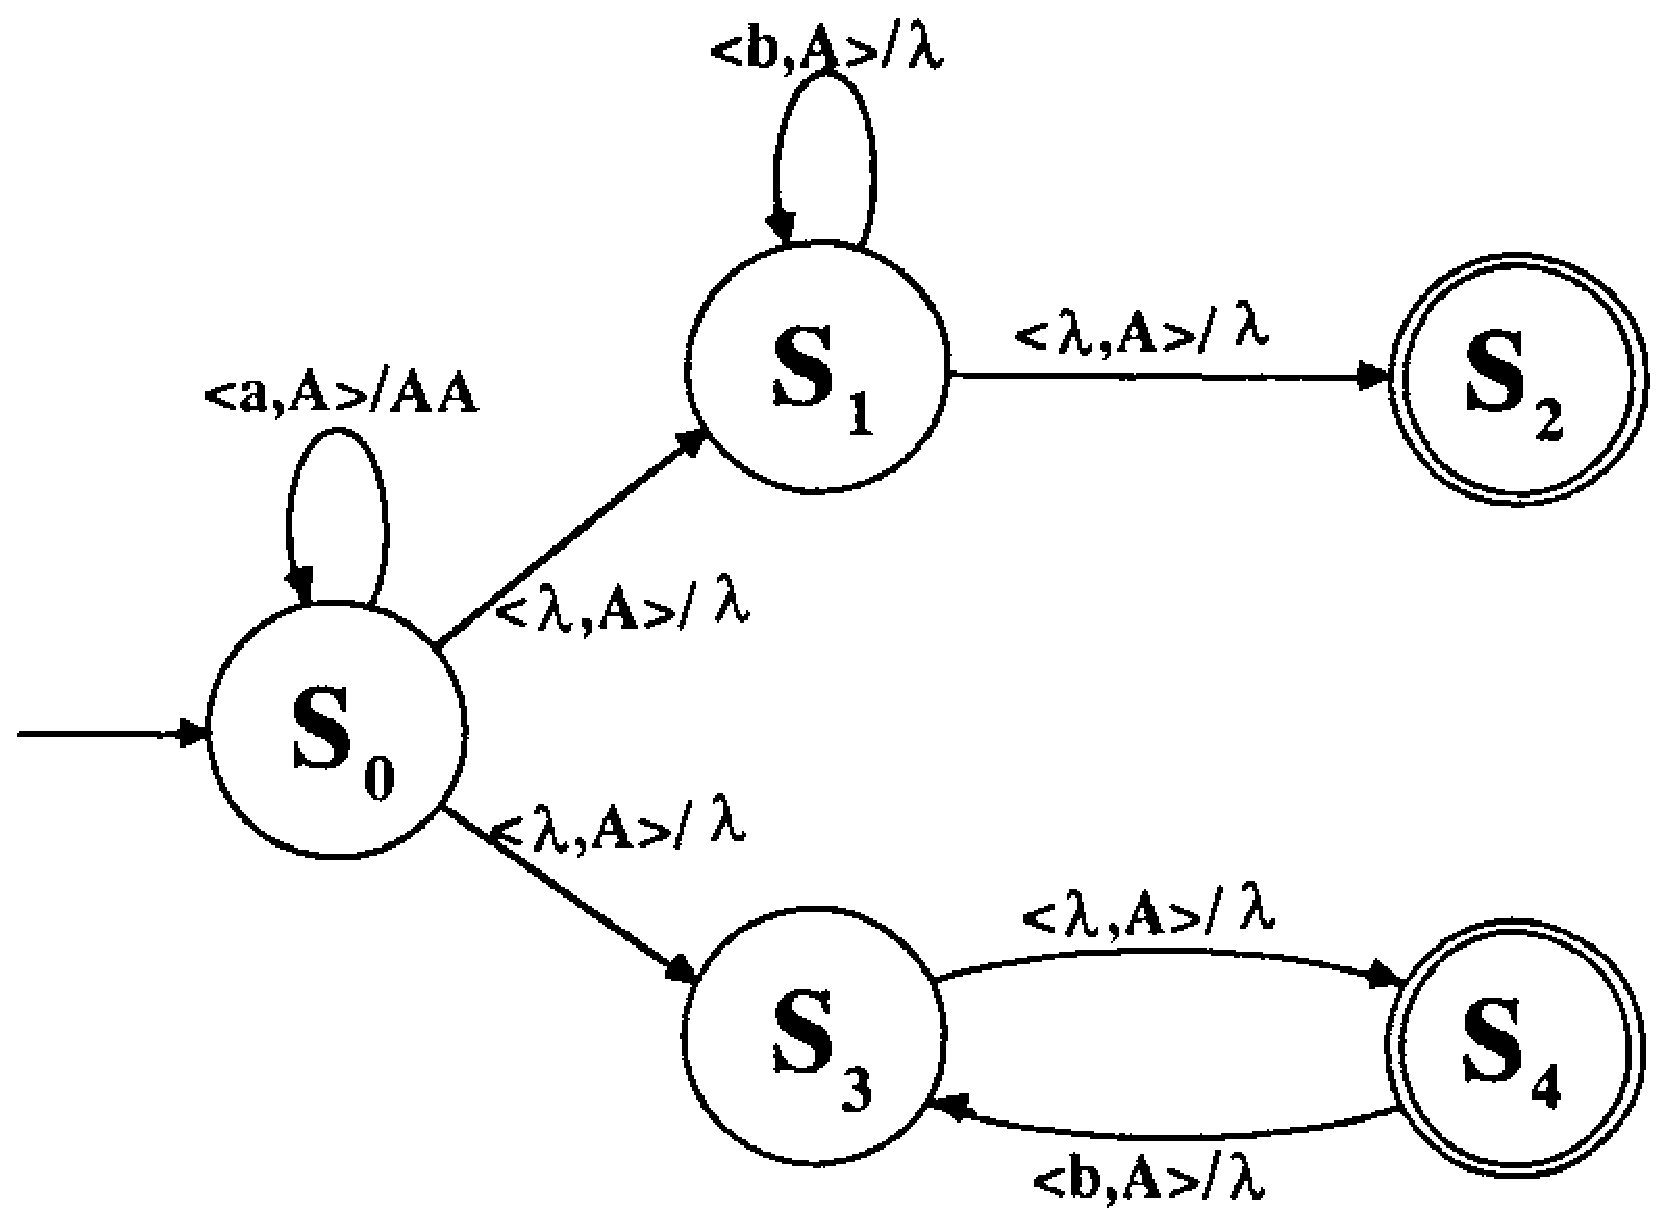
\epsfig{figure=ToFAfigures/fig10-4.eps,height=3.0in}}
\caption{The PDA discussed in Example 10.5}\label{fig-10.4}
\end{figure}

Since $A$ was the only stack symbol in $P_3$, the language could have as easily
been described by the sack-and-stone counting device described at the beginning
of the section. It should be clear that counting automata are essentially
pushdown automata with a singleton stack alphabet. Pushdown automata with only
one stack symbol cannot generate all the languages that a PDA with two symbols
can [DENN]. However, it can be shown that using more than two stack symbols does
not contribute to the generative power of a PDA; for example, a PDA with
$\Gamma=\{A,B,C,D\}$ can be converted into an equivalent machine with $\Gamma'=
\{0,1\}$ and the occurrences of the old stack symbols replaced by the encodings
$A=01,\ B=001,\ C=0001$, and $D=00001$.

Every NDFA can be simulated by a PDA that simply ignores its stack. In fact,
every NDFA has an equivalent counting automaton, as shown in the following
theorem.

% Theorem 10.1
\begin{thm}\label{thm-10.1}\index{equivalent!PDAs}\index{NDFA}
Given any alphabet $\Sigma$, and an NDFA $A$:
\begin{enumerate}
\item There is an equivalent pushdown automaton (counting automaton) $A'$ for
which $L(A)=L(A')$.
\item There is an equivalent pushdown automaton (counting automaton) $A''$ for
which $L(A)=\Lambda(A'')$.
\end{enumerate}

\emph{Proof.} The results for pushdown automata will actually follow from the
results of the next section, since pushdown automata can define all the
context-free languages, and the regular language defined by the NDFA $A$ must be
context free. The following constructions will use only the one stack symbol
\cent, and hence $A'$ and $A''$ are actually \emph{counting} automata for which $L(A)=
L(A')$ and $L(A)=\Lambda(A'')$.

While the construction of a PDA from an NDFA is straightforward, the inductive
proofs are simplified if we appeal to Theorem \ref{thm-4.1}, and assume that the given
automaton is actually a DFA $A=\langle\Sigma,S,s_0,\delta,F\rangle$. Define the
PDA $A'=\langle\Sigma,\{\cent\},S,s_0,\delta',\cent,F\rangle$, where $\delta'$
is defined by
\[ (\forall s\in S)(\forall \pmb{a}\in\Sigma)(\delta'(s,\pmb{a},\cent)=\{\langle
	\delta(s,\pmb{a}),\cent\rangle\}) \]
and $(\forall s\in S)(\delta'(s,\lambda,\cent)=\{\ \ \})$. That is, the PDA makes
the same transitions that the DFA does and replaces the \cent\ with the same
symbol on the stack at each move. The proof that $A$ and $A'$ are equivalent is
by induction on the length of the input string, where $P(n)$ is the statement
that
\[ (\forall x\in\Sigma^n)(\DBAR(s_0,x)=t\Leftrightarrow\langle s_0,x,\cent
	\rangle\Dvdash\langle t,\lambda,\cent\rangle) \]
The PDA with a single stack symbol that accepts $L$ via empty stack is quite
similar; final states are simply given the added option of removing the only
symbol on the stack. That is, $A''=\langle\Sigma,\{\cent\},S,s_0,\delta'',\cent,
\emptyset\rangle$, where $\delta''$ is defined by
\[ (\forall s\in S)(\forall\pmb{a}\in\Sigma)(\delta''(s,\pmb{a},\cent)=\{\langle
	\delta(s,\pmb{a}),\cent\rangle\}) \]
and
\[ (\forall s\in F)(\delta''(s,\lambda,\cent)=\{\langle s,\lambda\rangle\}) \]
while
\[ (\forall s\in S-F)(\delta''(s,\lambda,\cent)=\{\ \ \}) \]
The same type of inductive statement proved for $A'$ holds for $A''$, and it
therefore will follow that exactly those words that terminate in what used to be
final states empty the stack, and thus $L(A)=\Lambda(A'')$.
\end{thm}

\section{Equivalence of PDAs and CFGs}\label{sec-10.2}

In this section, it will be shown that if $L$ is accepted by a PDA, then $L$ can
be generated by a CFG, and, conversely, every context-free language can be
recognized by a PDA. We will also show that the class of pushdown automata that
accept by empty stack defines exactly the same languages as the class of
pushdown automata that accept by final state. In each case, the languages
defined are exactly the context-free languages.

% Definition 10.5
\begin{dfn}\label{dfn-10.5}\index{P@\PSIG \ (P-sigma )}\index{F@\FSIG \ (F-sigma )}
For a given alphabet $\Sigma$, let
\begin{center}\begin{tabular}{l}
$\PSIG = \{L \subseteq \Sigma^*|\ \exists\text{PDA }P \ni L = \Lambda(P)\}$ \\
$\FSIG = \{L \subseteq \Sigma^*|\ \exists\text{PDA }P \ni L = L(P)\}$
\end{tabular}\end{center}
\end{dfn}

Recall that \CSIG\ was defined to be the collection of context-free languages. We
begin by showing that $\CSIG\subseteq\PSIG$. To do this, we must show that,
given a language $L$ generated by a context-free grammar $G$, there is a PDA
$P_G$ that recognizes exactly those words that belong to $L$. The pushdown
automaton given in the next definition simulates leftmost derivations in $G$.
That is, as the symbols on the input tape are scanned, the automaton guesses at
the production that produced that letter and remembers the remainder of the
sentential form by pushing it on the stack. $P_G$ is constructed in such a way
that, when the stack contents are checked against the symbols on the input tape,
wrong guesses are discovered and the device halts. Wrong guesses, corresponding
to inappropriate or impossible derivations, are thereby prevented from emptying
the stack, and yet each word that can be generated by $G$ will be guaranteed to
have a sequence of moves that results in acceptance by empty stack.

% Definition 10.6
\begin{dfn}\label{dfn-10.6}
Given a context-free grammar $G=\langle\Omega,\Sigma,S,P\rangle$ in pure
Greibach normal form, the single-state \emph{pushdown automaton corresponding to} $G$
is the septuple
\[ P_G=\langle\Sigma,\Omega\cup\Sigma,\{s\},s,\delta_G,S,\emptyset\rangle, \]
where $\delta_G$ is defined by

\begin{center}\begin{tabular}{r@{ = }l}
$\delta_G(s,\pmb{a},\Psi)$ & $\left\{\begin{tabular}{l@{$\qquad$}l@{$\qquad$}l}
	$\{\langle s,\alpha\rangle\ |\ \Psi\rightarrow\pmb{a}\alpha\in P\},$ &
		if \  $\Psi\in\Omega$ \\
	&& $\forall\pmb{a}\in\Sigma,\forall\Psi\in(\Omega\cup\Sigma)$ \\
	$\{\langle s,\lambda\rangle\},$ & if \  $\Psi\in\Sigma\wedge\Psi=\pmb{a}$
	\end{tabular}\right.$
\end{tabular}\end{center}
\end{dfn}

\subsection*{Example 10.6}\label{ex-10.6}

Consider the pure Greibach normal form grammar
\[ G=\langle\{S\},\{\pmb{a},\pmb{b}\},S,\{S\rightarrow\pmb{a}S\pmb{b},S
	\rightarrow\pmb{ab}\}\rangle \]
which is perhaps the simplest grammar generating $\{\pmb{a}^n\pmb{b}^n|\ n\geq 1\}$.
The automaton $P_G$ is then
\[ P_G = \langle\{\pmb{a},\pmb{b}\},\{S,\pmb{a},\pmb{b}\},\{s\},s,\delta_G,S,
	\emptyset\rangle \]
where $\delta_G$ is defined by
\begin{center}\begin{tabular}{l}
$\delta_G(s,\pmb{a},S)=\{\langle s,S\pmb{b}\rangle,\langle s,\pmb{b}\rangle\}$ \\
$\delta_G(s,\pmb{a},\pmb{a})=\{\langle s,\lambda\rangle\}$ \\
$\delta_G(s,\pmb{a},\pmb{b})=\{\ \ \}$ \\
$\delta_G(s,\pmb{b},S)=\{\ \ \}$ \\
$\delta_G(s,\pmb{b},\pmb{a})=\{\ \ \}$ \\
$\delta_G(s,\pmb{b},\pmb{b})=\{\langle s,\lambda\rangle\}$
\end{tabular}\end{center}
This automaton contains no $\lambda$-moves and is essentially the same as $P_2$
in Example 10.4, with the state $t$ now relabeled as $s$, the stack symbol
$\pmb{b}$ now playing the role of $C$, and the unused stack symbol $\pmb{a}$ added
to $\Gamma$. The derivation $S\Rightarrow\pmb{a}S\pmb{b}\Rightarrow\pmb{aabb}$
corresponds to the successful move sequence
\[ \langle s,\pmb{aabb},S\rangle\vdash\langle s,\pmb{abb},S\pmb{b}\rangle\vdash
	\langle s,\pmb{bb},\pmb{bb}\rangle\vdash\langle s,\pmb{b},\pmb{b}\rangle
	\vdash\langle s,\lambda,\lambda\rangle. \]
The exact correspondence between derivation steps and move sequences is
illustrated in the next example.

\subsection*{Example 10.7}

For a slightly more complex example, consider the pure Greibach normal form
grammar
\[ G = \langle\{R\},\{\pmb{a},\pmb{b},\pmb{c},\pmb{(},\pmb{)},\pmb{\epsilon},
	\pmb{\emptyset},\pmb{\cup},\pmb{\cdot},\pmb{^*}\},R,\{R\rightarrow
	\pmb{a}|\pmb{b}|\pmb{c}|\pmb{\epsilon}|\pmb{\emptyset}|(R\pmb{\cdot}R)|
	(R\pmb{\cup}R)|(R)\pmb{^*}\}\rangle. \]
The automaton $P_G$ is then
\[ \langle\{\pmb{a},\pmb{b},\pmb{c},\pmb{(},\pmb{)},\pmb{\epsilon},
	\pmb{\emptyset},\pmb{\cup},\pmb{\cdot},^{\pmb{*}}\},\{R,\pmb{a},\pmb{b},
	\pmb{c},\pmb{(},\pmb{)},\pmb{\epsilon},\pmb{\emptyset},\pmb{\cup},
	\pmb{\cdot},^{\pmb{*}}\},\{s\},s,\delta_G,R,\emptyset\rangle, \]
where $\delta_G$ is comprised of the following nonempty transitions:
\begin{center}\begin{tabular}{r@{ = }l}
$\delta_G(s,\pmb{(},R)$ & $\{\langle s,R\pmb{\cdot}R\pmb{)}\rangle,\langle s,R
	\pmb{\cup}R\pmb{)}\rangle,\langle s,R\pmb{)}^{\pmb{*}}\rangle\}$ \\
$\delta_G(s,\pmb{a},R)$ & $\{\langle s,\lambda\rangle\}$ \\
$\delta_G(s,\pmb{b},R)$ & $\{\langle s,\lambda\rangle\}$ \\
$\delta_G(s,\pmb{c},R)$ & $\{\langle s,\lambda\rangle\}$ \\
$\delta_G(s,\pmb{\epsilon},R)$ & $\{\langle s,\lambda\rangle\}$ \\
$\delta_G(s,\pmb{\emptyset},R)$ & $\{\langle s,\lambda\rangle\}$ \\
$\delta_G(s,\pmb{a},\pmb{a})$ & $\{\langle s,\lambda\rangle\}$ \\
$\delta_G(s,\pmb{b},\pmb{b})$ & $\{\langle s,\lambda\rangle\}$ \\
$\delta_G(s,\pmb{c},\pmb{c})$ & $\{\langle s,\lambda\rangle\}$ \\
$\delta_G(s,\pmb{\emptyset},\pmb{\emptyset})$ & $\{\langle s,\lambda\rangle\}$ \\
$\delta_G(s,\pmb{\epsilon},\pmb{\epsilon})$ & $\{\langle s,\lambda\rangle\}$ \\
$\delta_G(s,\pmb{\cup},\pmb{\cup})$ & $\{\langle s,\lambda\rangle\}$ \\
$\delta_G(s,\pmb{\cdot},\pmb{\cdot})$ & $\{\langle s,\lambda\rangle\}$ \\
$\delta_G(s,\pmb{^*},\pmb{^*})$ & $\{\langle s,\lambda\rangle\}$ \\
$\delta_G(s,\pmb{)},\pmb{)})$ & $\{\langle s,\lambda\rangle\}$ \\
$\delta_G(s,\pmb{(},\pmb{(})$ & $\{\langle s,\lambda\rangle\}$ \\
\end{tabular}\end{center}
In this grammar, it happens that the symbol $\pmb{(}$ is never pushed onto the
stack, and so the last transition is not utilized. Transitions not listed are
empty; that is, they are of the form $\delta_G(s,\pmb{d},A)=\{\ \ \}$.

Consider the string $\pmb{(a\cup(b\cdot c))}$, which has the following (unique)
derivation:
\begin{center}\begin{tabular}{r@{ $\Rightarrow$ }l}
$R$ & $\pmb{(}R\pmb{\cup}R\pmb{)}$ \\
& $\pmb{(a\cup}R\pmb{)}$ \\
& $\pmb{(a\cup(}R\pmb{\cdot}R\pmb{))}$ \\
& $\pmb{(a\cup(b}\pmb{\cdot}R\pmb{))}$ \\
& $\pmb{(a\cup(b\cdot c))}$
\end{tabular}\end{center}
$P_G$ simulates this derivation with the following steps:
\begin{center}\begin{tabular}{r@{ $\vdash$ }l}
$\langle s,\pmb{(a\cup(b\cdot c))},R)\rangle$ & $\langle s,\pmb{a\cup(b\cdot
	c))},R\pmb{\cup}R\pmb{)}\rangle$ \\
& $\langle s,\pmb{\cup(b\cdot c))},\pmb{\cup}R\pmb{)}\rangle$ \\
& $\langle s,\pmb{(b\cdot c))},R\pmb{)}\rangle$ \\
& $\langle s,\pmb{b\cdot c))},R\pmb{\cdot}R\pmb{))}\rangle$ \\
& $\langle s,\pmb{\cdot c))},\pmb{\cdot}R\pmb{))}\rangle$ \\
& $\langle s,\pmb{c))},R\pmb{))}\rangle$ \\
& $\langle s,\pmb{))},\pmb{))}\rangle$ \\
& $\langle s,\pmb{)},\pmb{)}\rangle$ \\
& $\langle s,\lambda,\lambda\rangle$
\end{tabular}\end{center}

Figures \ref{fig-10.5a}-f illustrates the state of the machine at several points during the
move sequence. At each point when an $R$ is the top stack symbol and the input
tape head is scanning a $\pmb{(}$, there are three choices of productions that
might have generated the opening parenthesis, and consequently the automaton has
three choices with which to replace the $R$ on the stack. If the wrong choice is
taken, $P_G$ will halt at some future point. For example, if the initial move
guessed that the first parenthesis was due to a concatenation operation, the
move sequence would be
\[ \langle s,\pmb{(a\cup(b\cdot c))},R\rangle\vdash\langle s,\pmb{a\cup(b\cdot
	c))},R\pmb{\cdot}R\pmb{)}\rangle\vdash\langle s,\pmb{\cup(b\cdot c))},
	\pmb{\cdot}R\pmb{)}\rangle \]
Since there are no $\lambda$-moves and the entry for $\delta_G(s,\pmb{\cup},
\pmb{\cdot})$ is empty, this attempt can go no further. A construction such as
the one given in Definition \ref{dfn-10.6} can be shown to produce the desired automaton
for any context-free grammar in Greibach normal form.

\setcounter{figure}{0}
\renewcommand{\thefigure}{\arabic{chapter}.5\alph{figure}}
% Figure 10.5a
\begin{figure}
\centerline{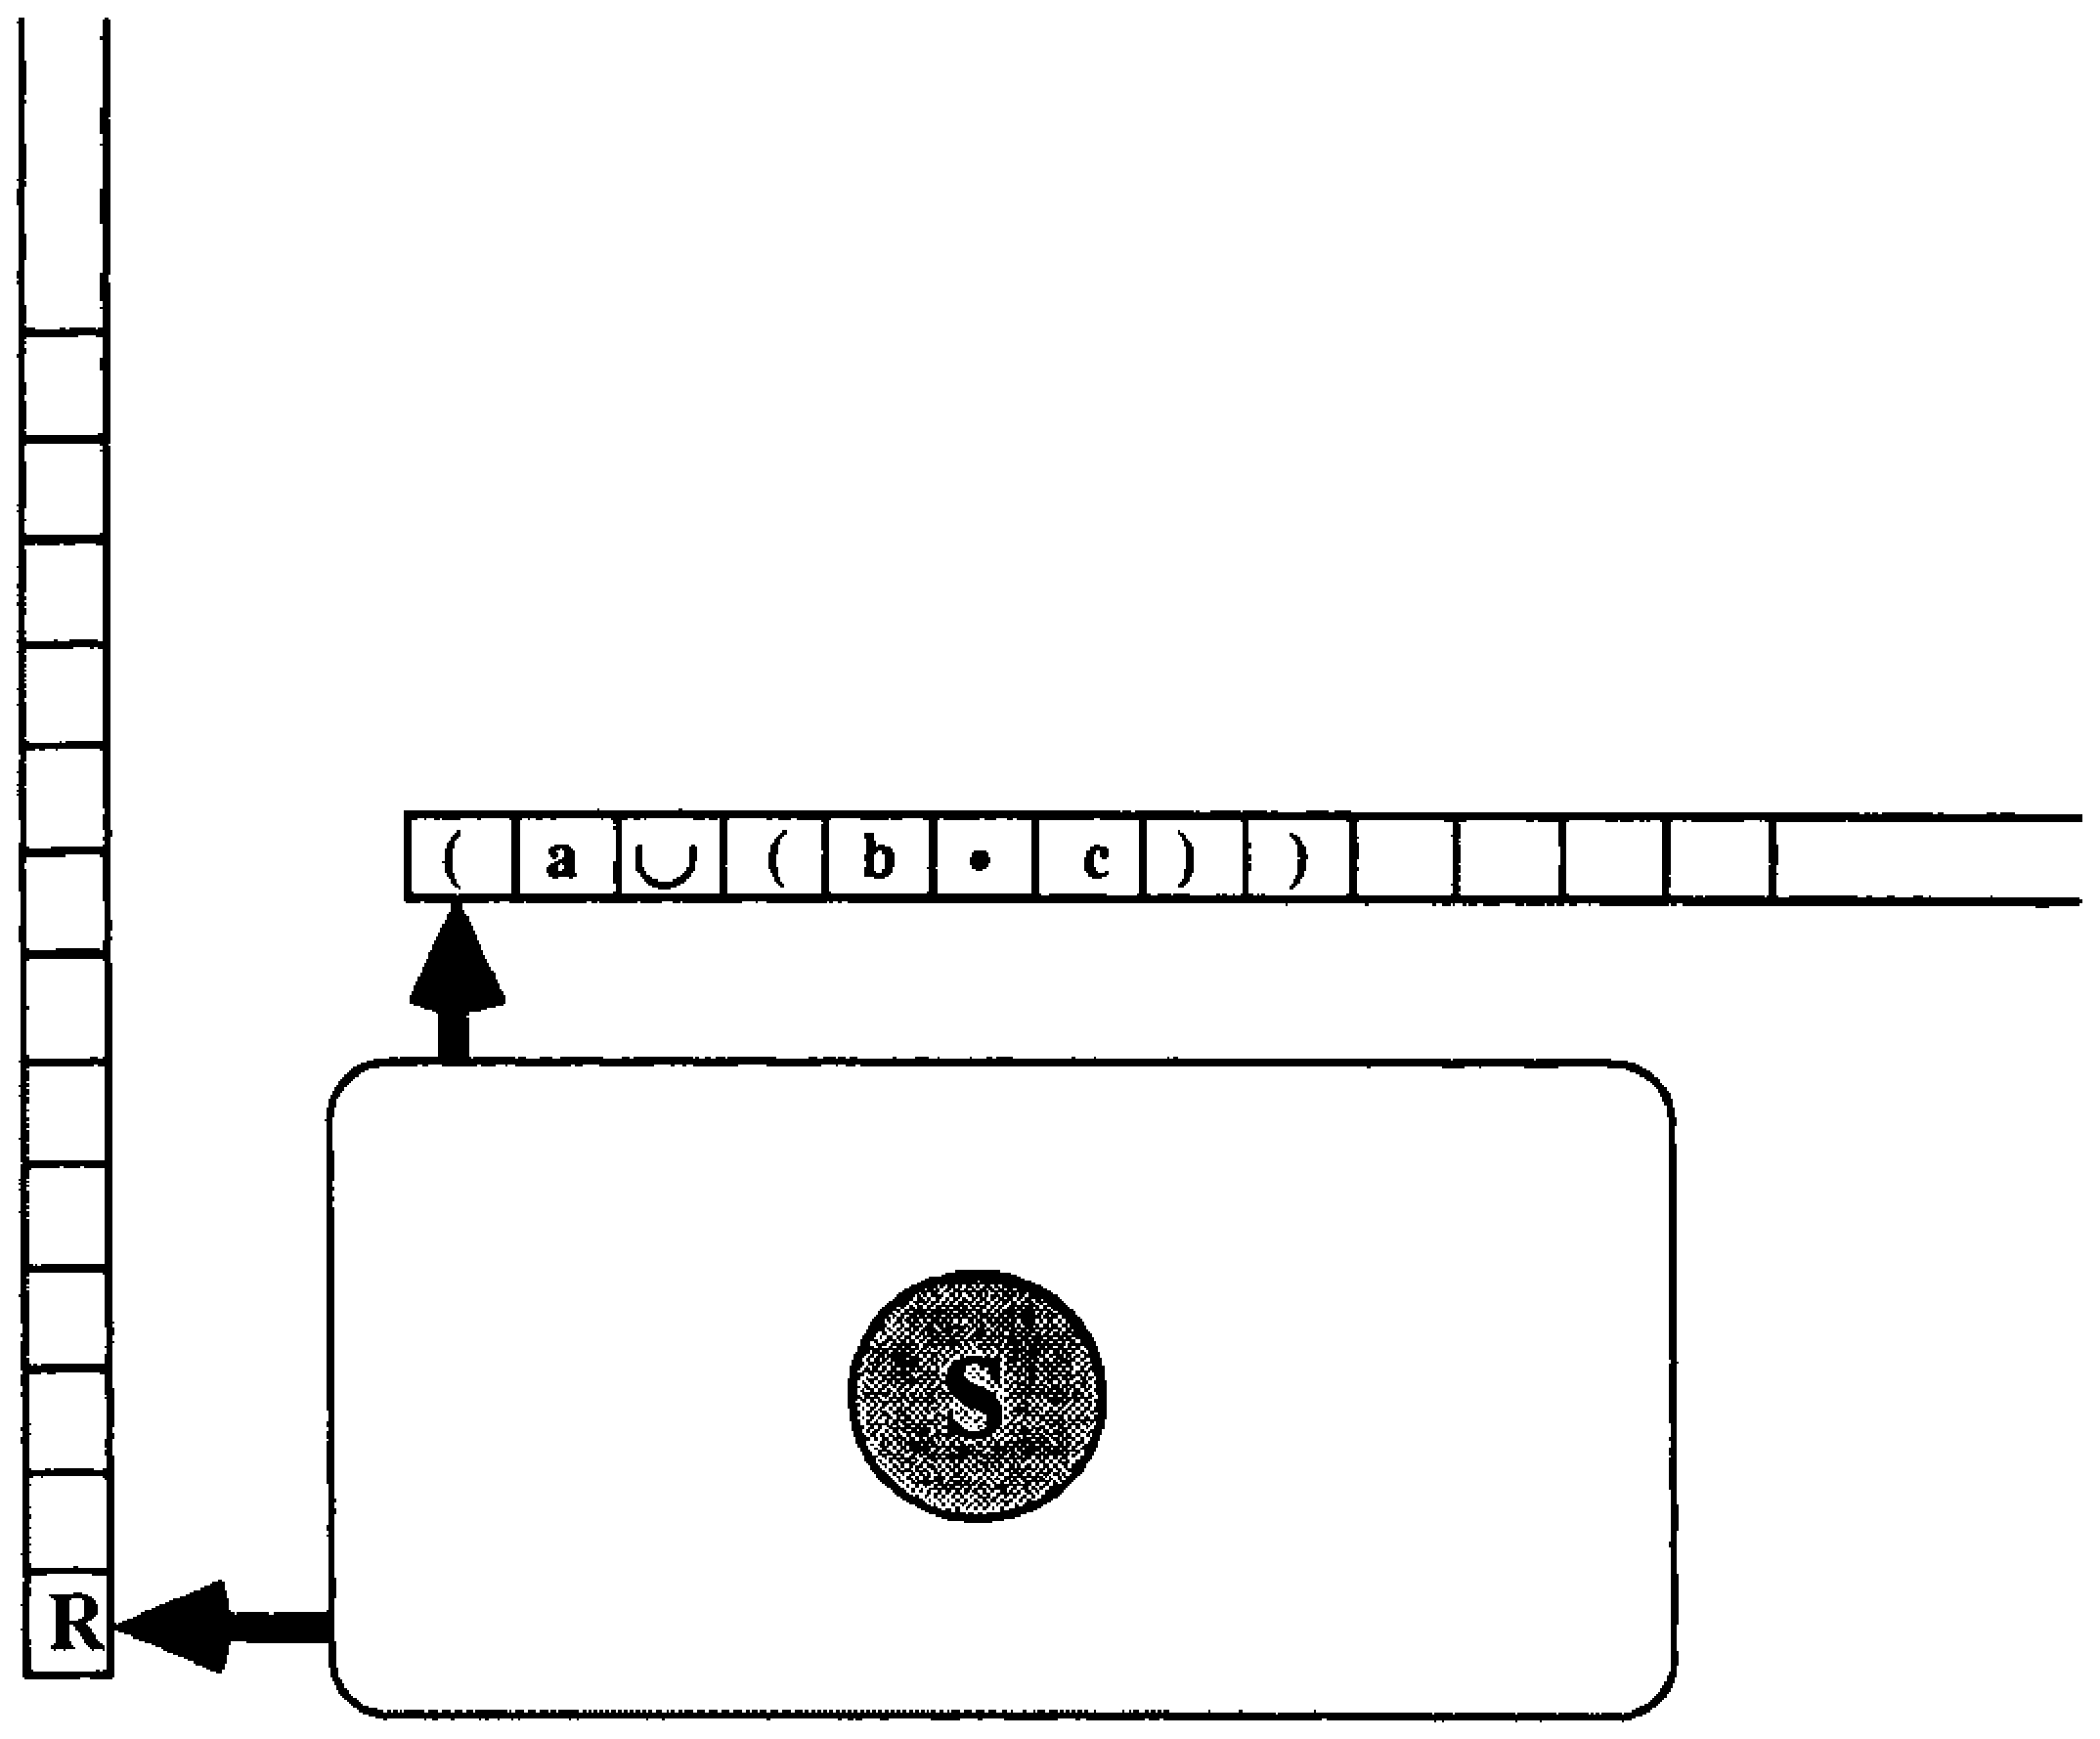
\epsfig{figure=ToFAfigures/fig10-5a.eps,height=2.0in}}
\caption{Walkthrough of the pushdown automaton discussed in Example 10.7}\label{fig-10.5a}
\end{figure}

% Figure 10.5b
\begin{figure}
\centerline{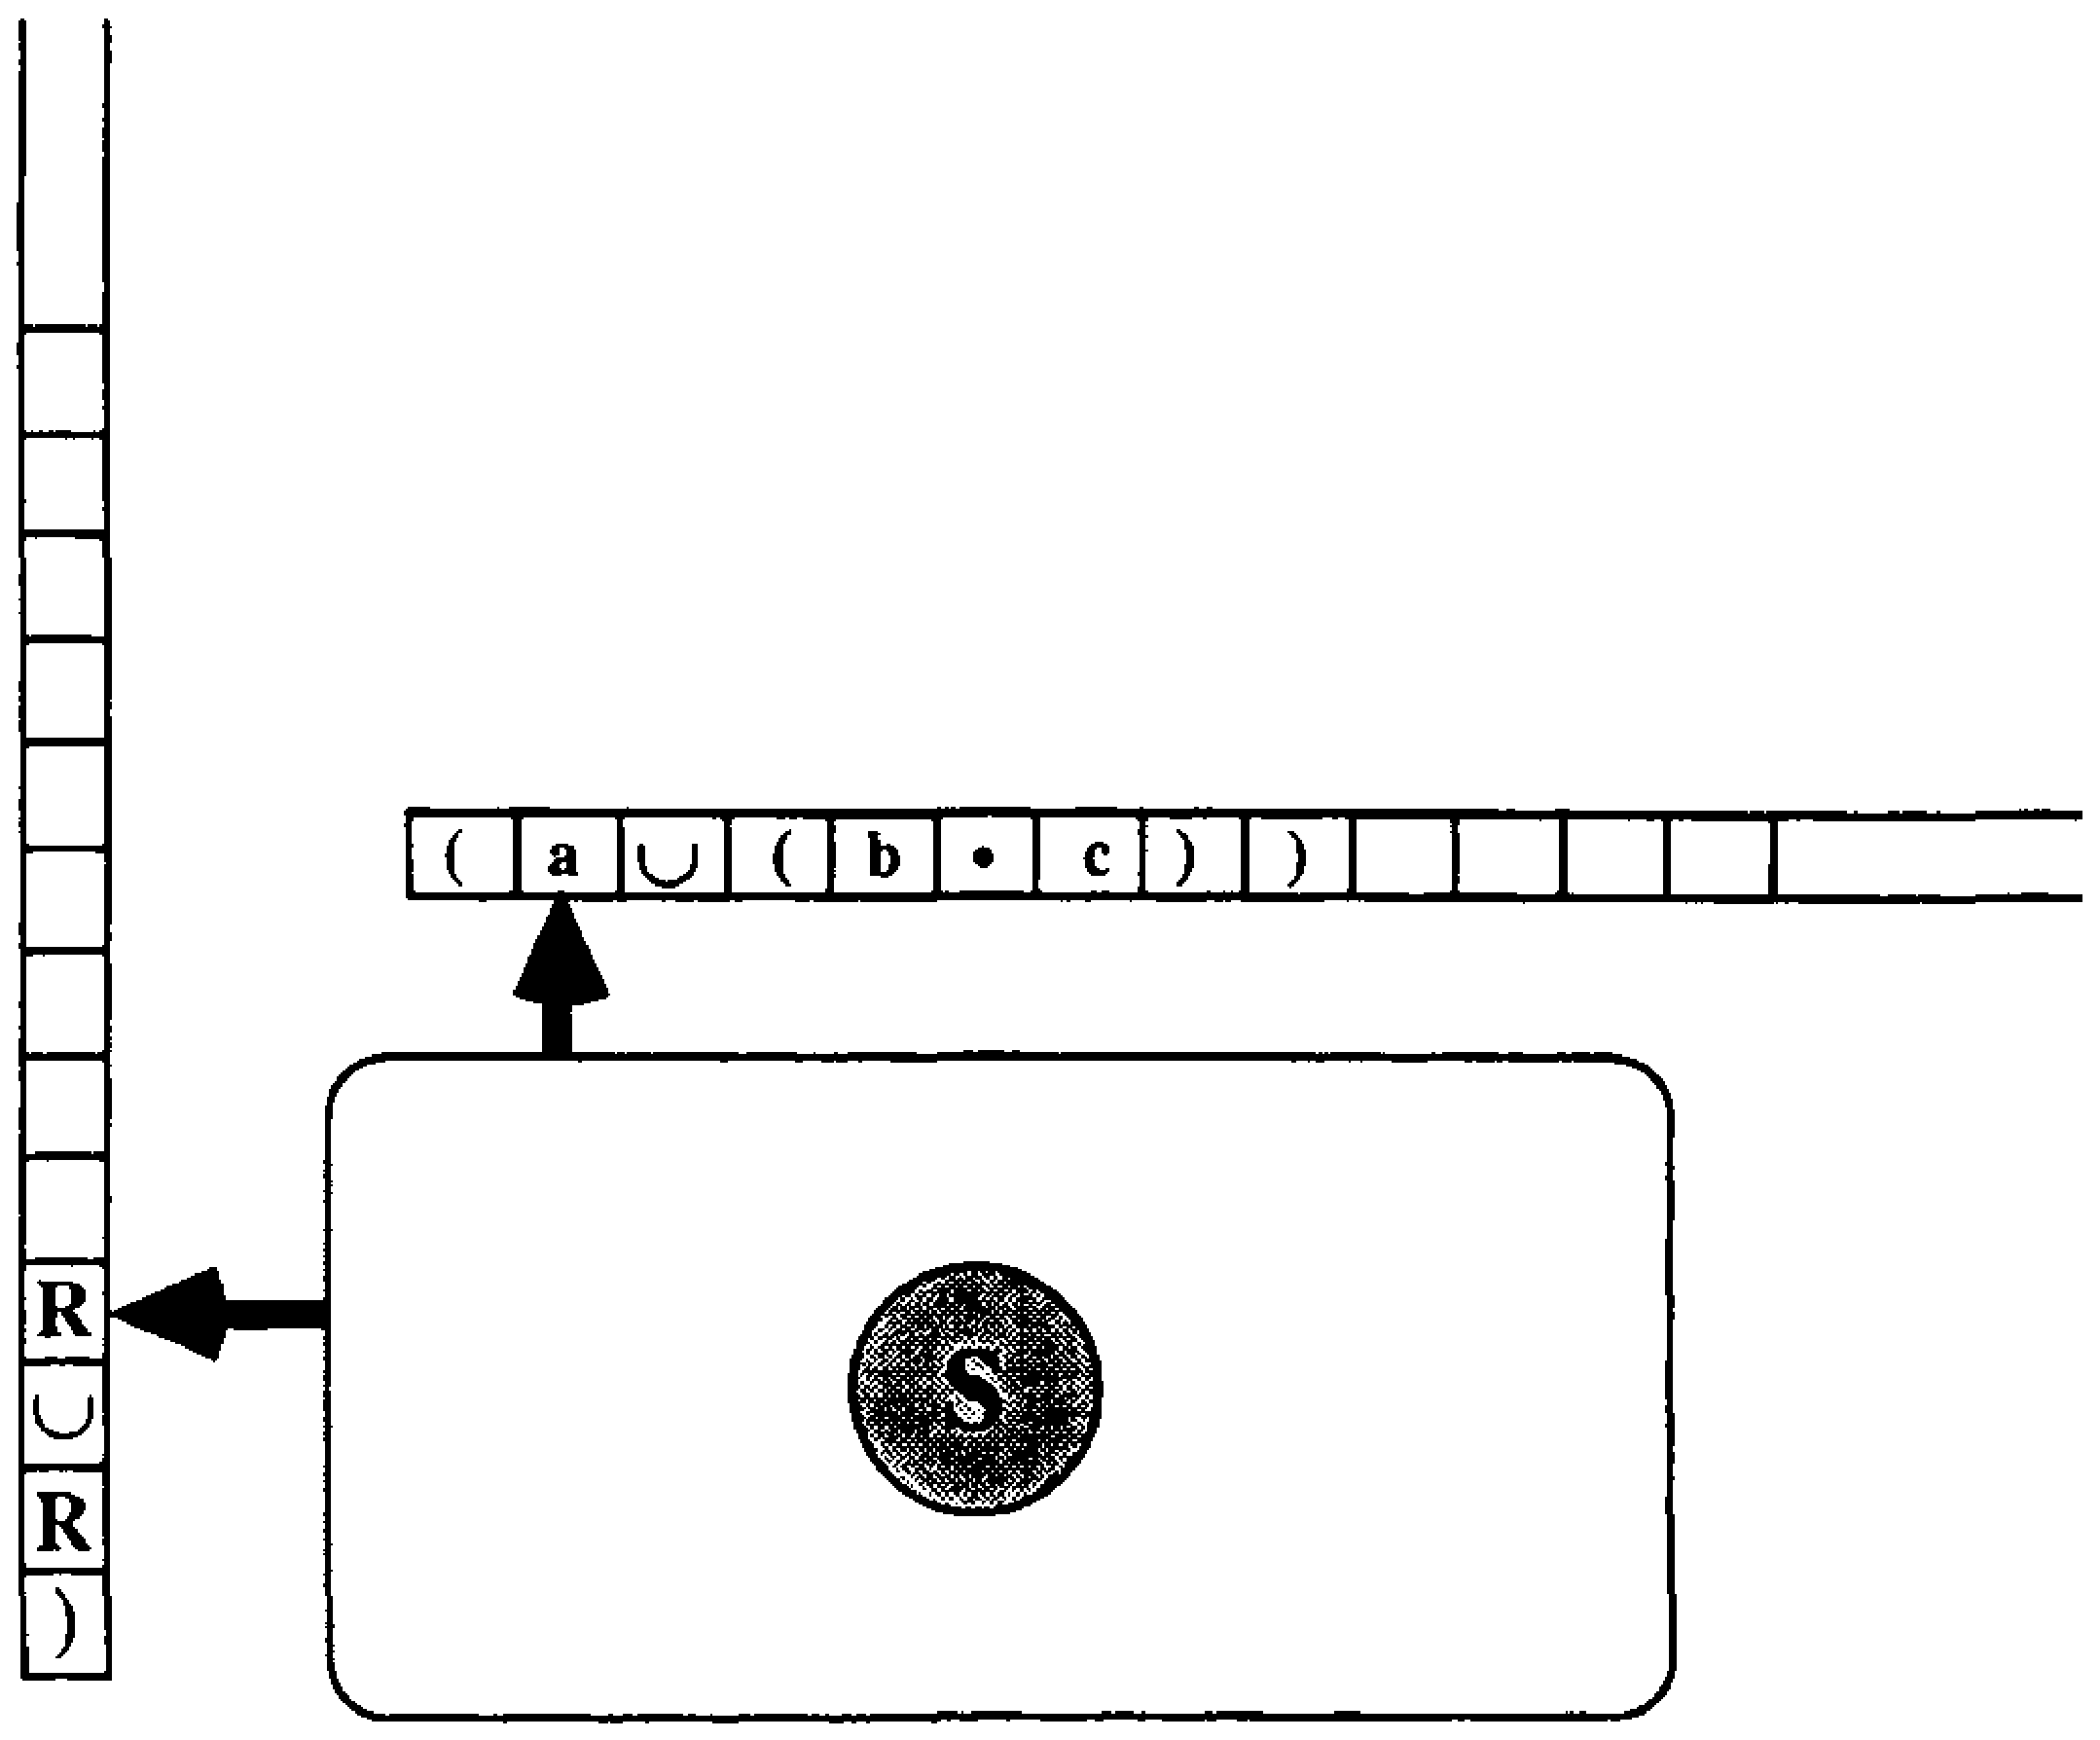
\epsfig{figure=ToFAfigures/fig10-5b.eps,height=2.0in}}
\caption{Walkthrough of the pushdown automaton discussed in Example 10.7}\label{fig-10.5b}
\end{figure}

% Figure 10.5c
\begin{figure}
\centerline{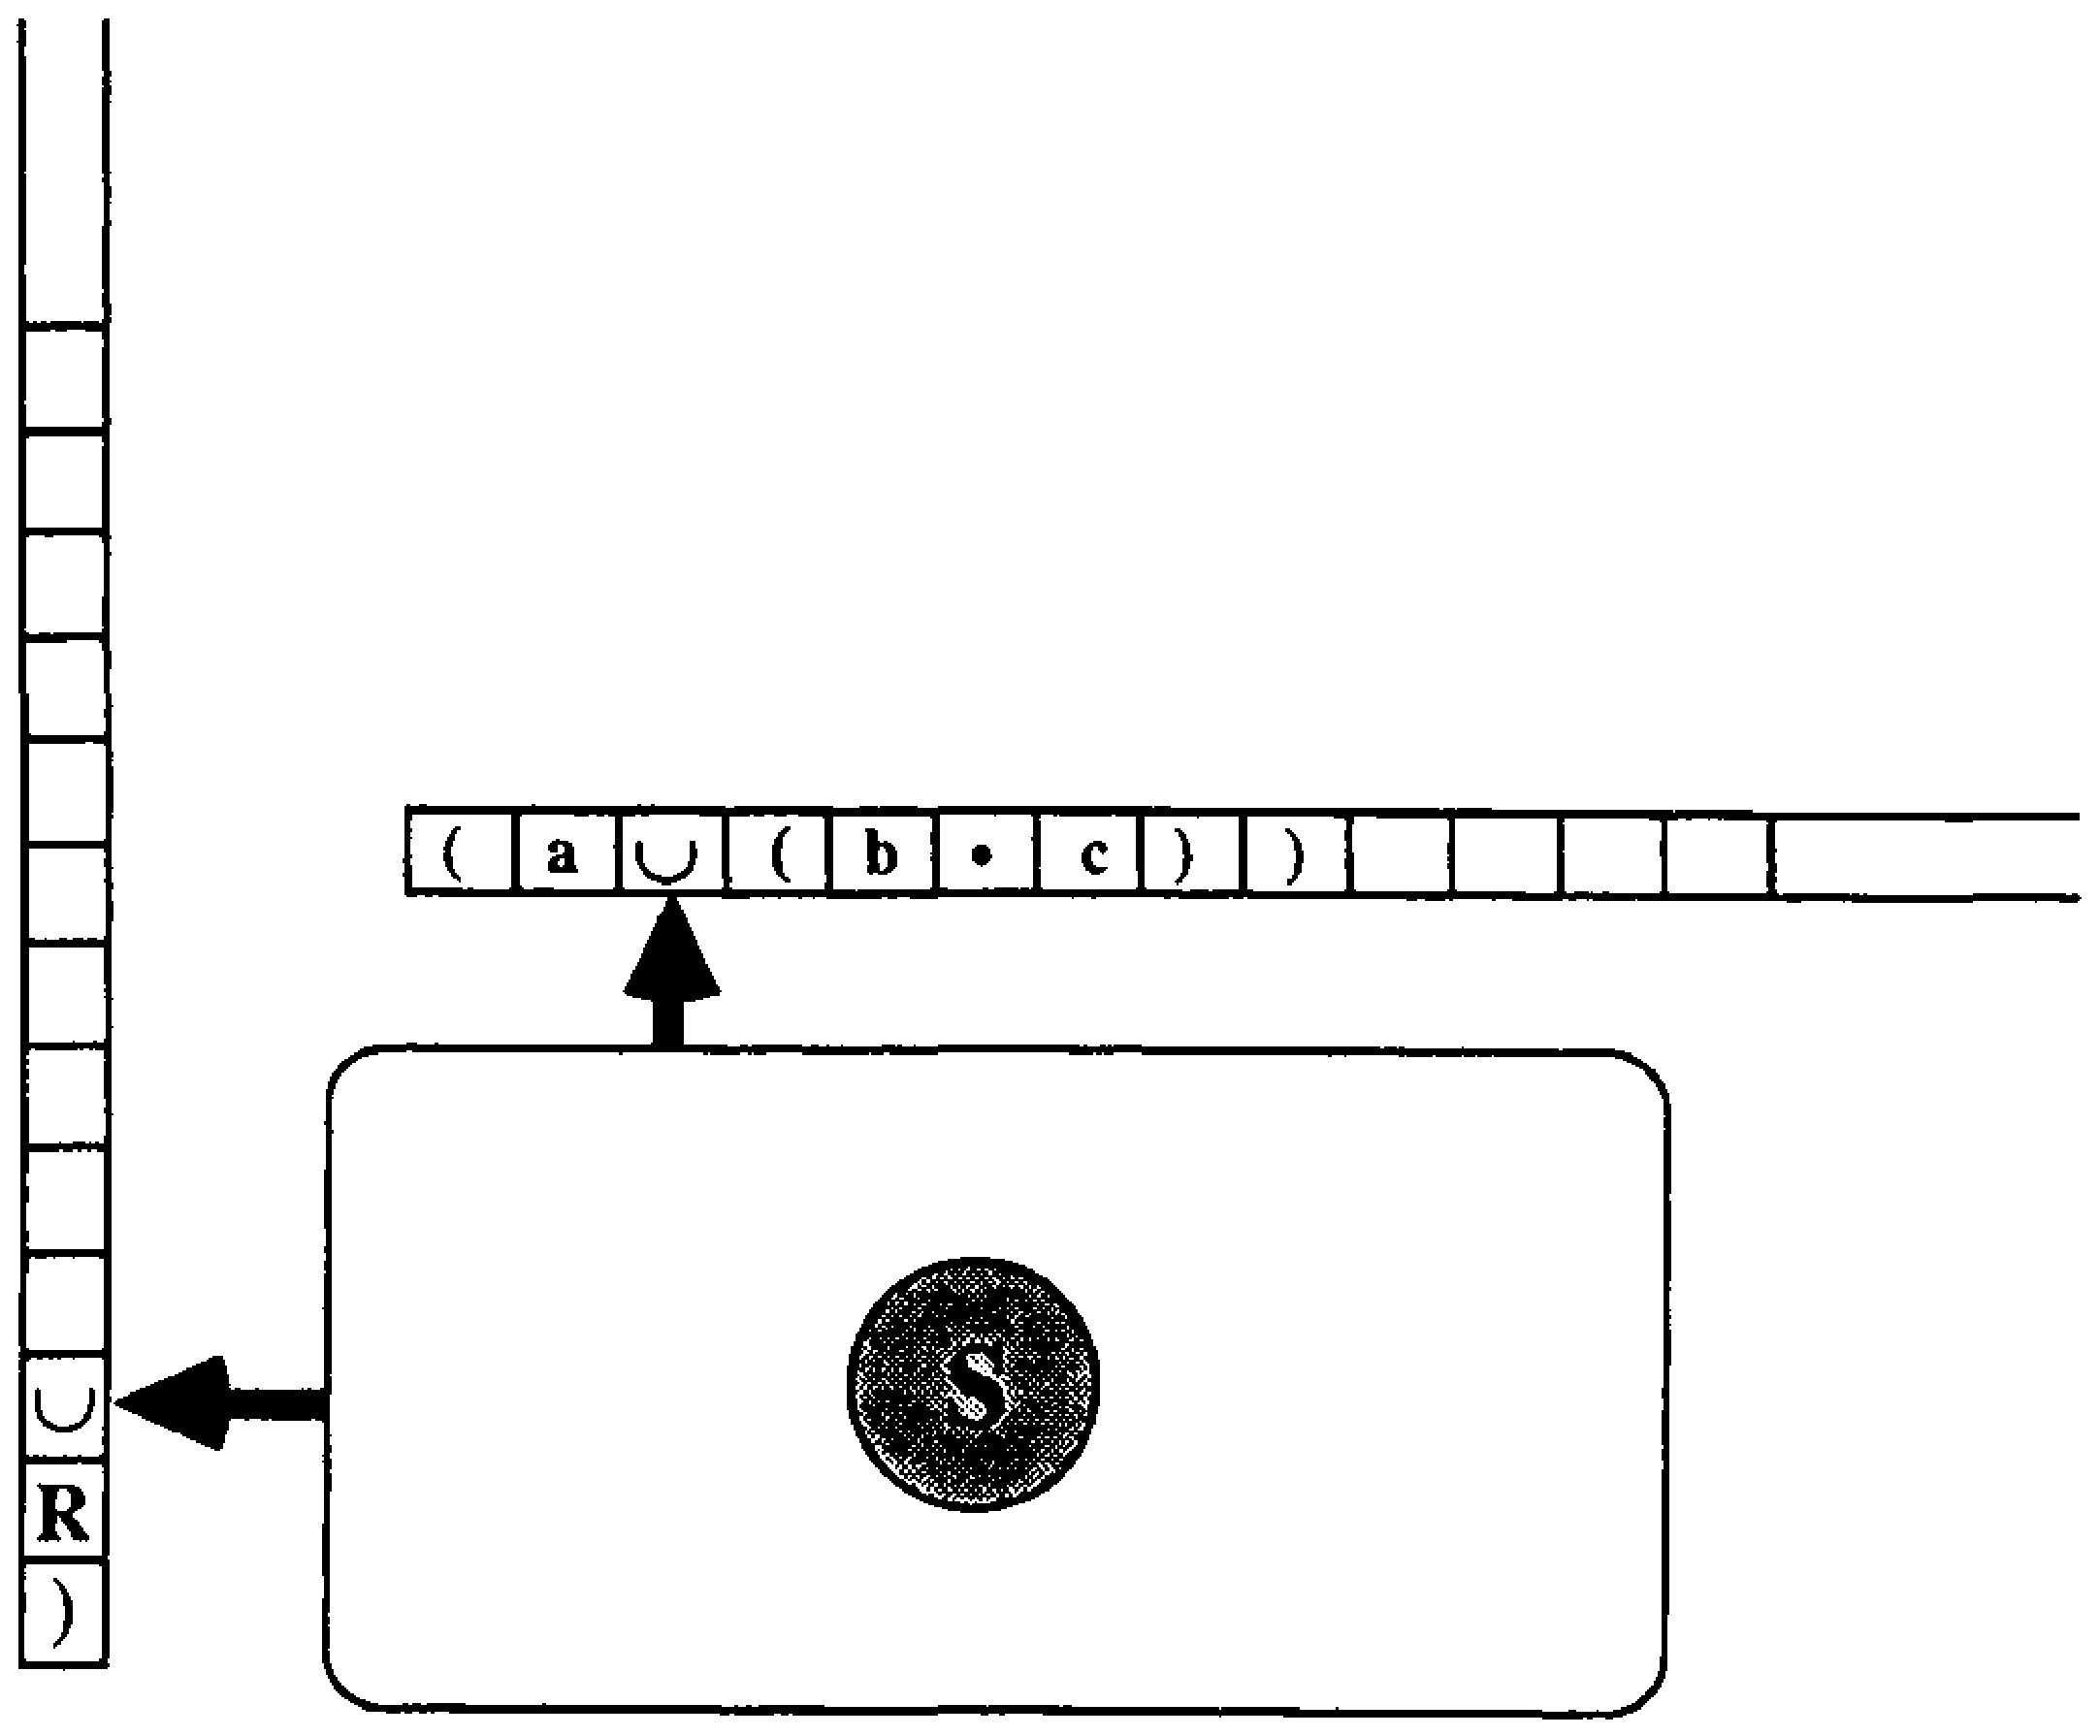
\epsfig{figure=ToFAfigures/fig10-5c.eps,height=2.0in}}
\caption{Walkthrough of the pushdown automaton discussed in Example 10.7}\label{fig-10.5c}
\end{figure}

% Figure 10.5d
\begin{figure}
\centerline{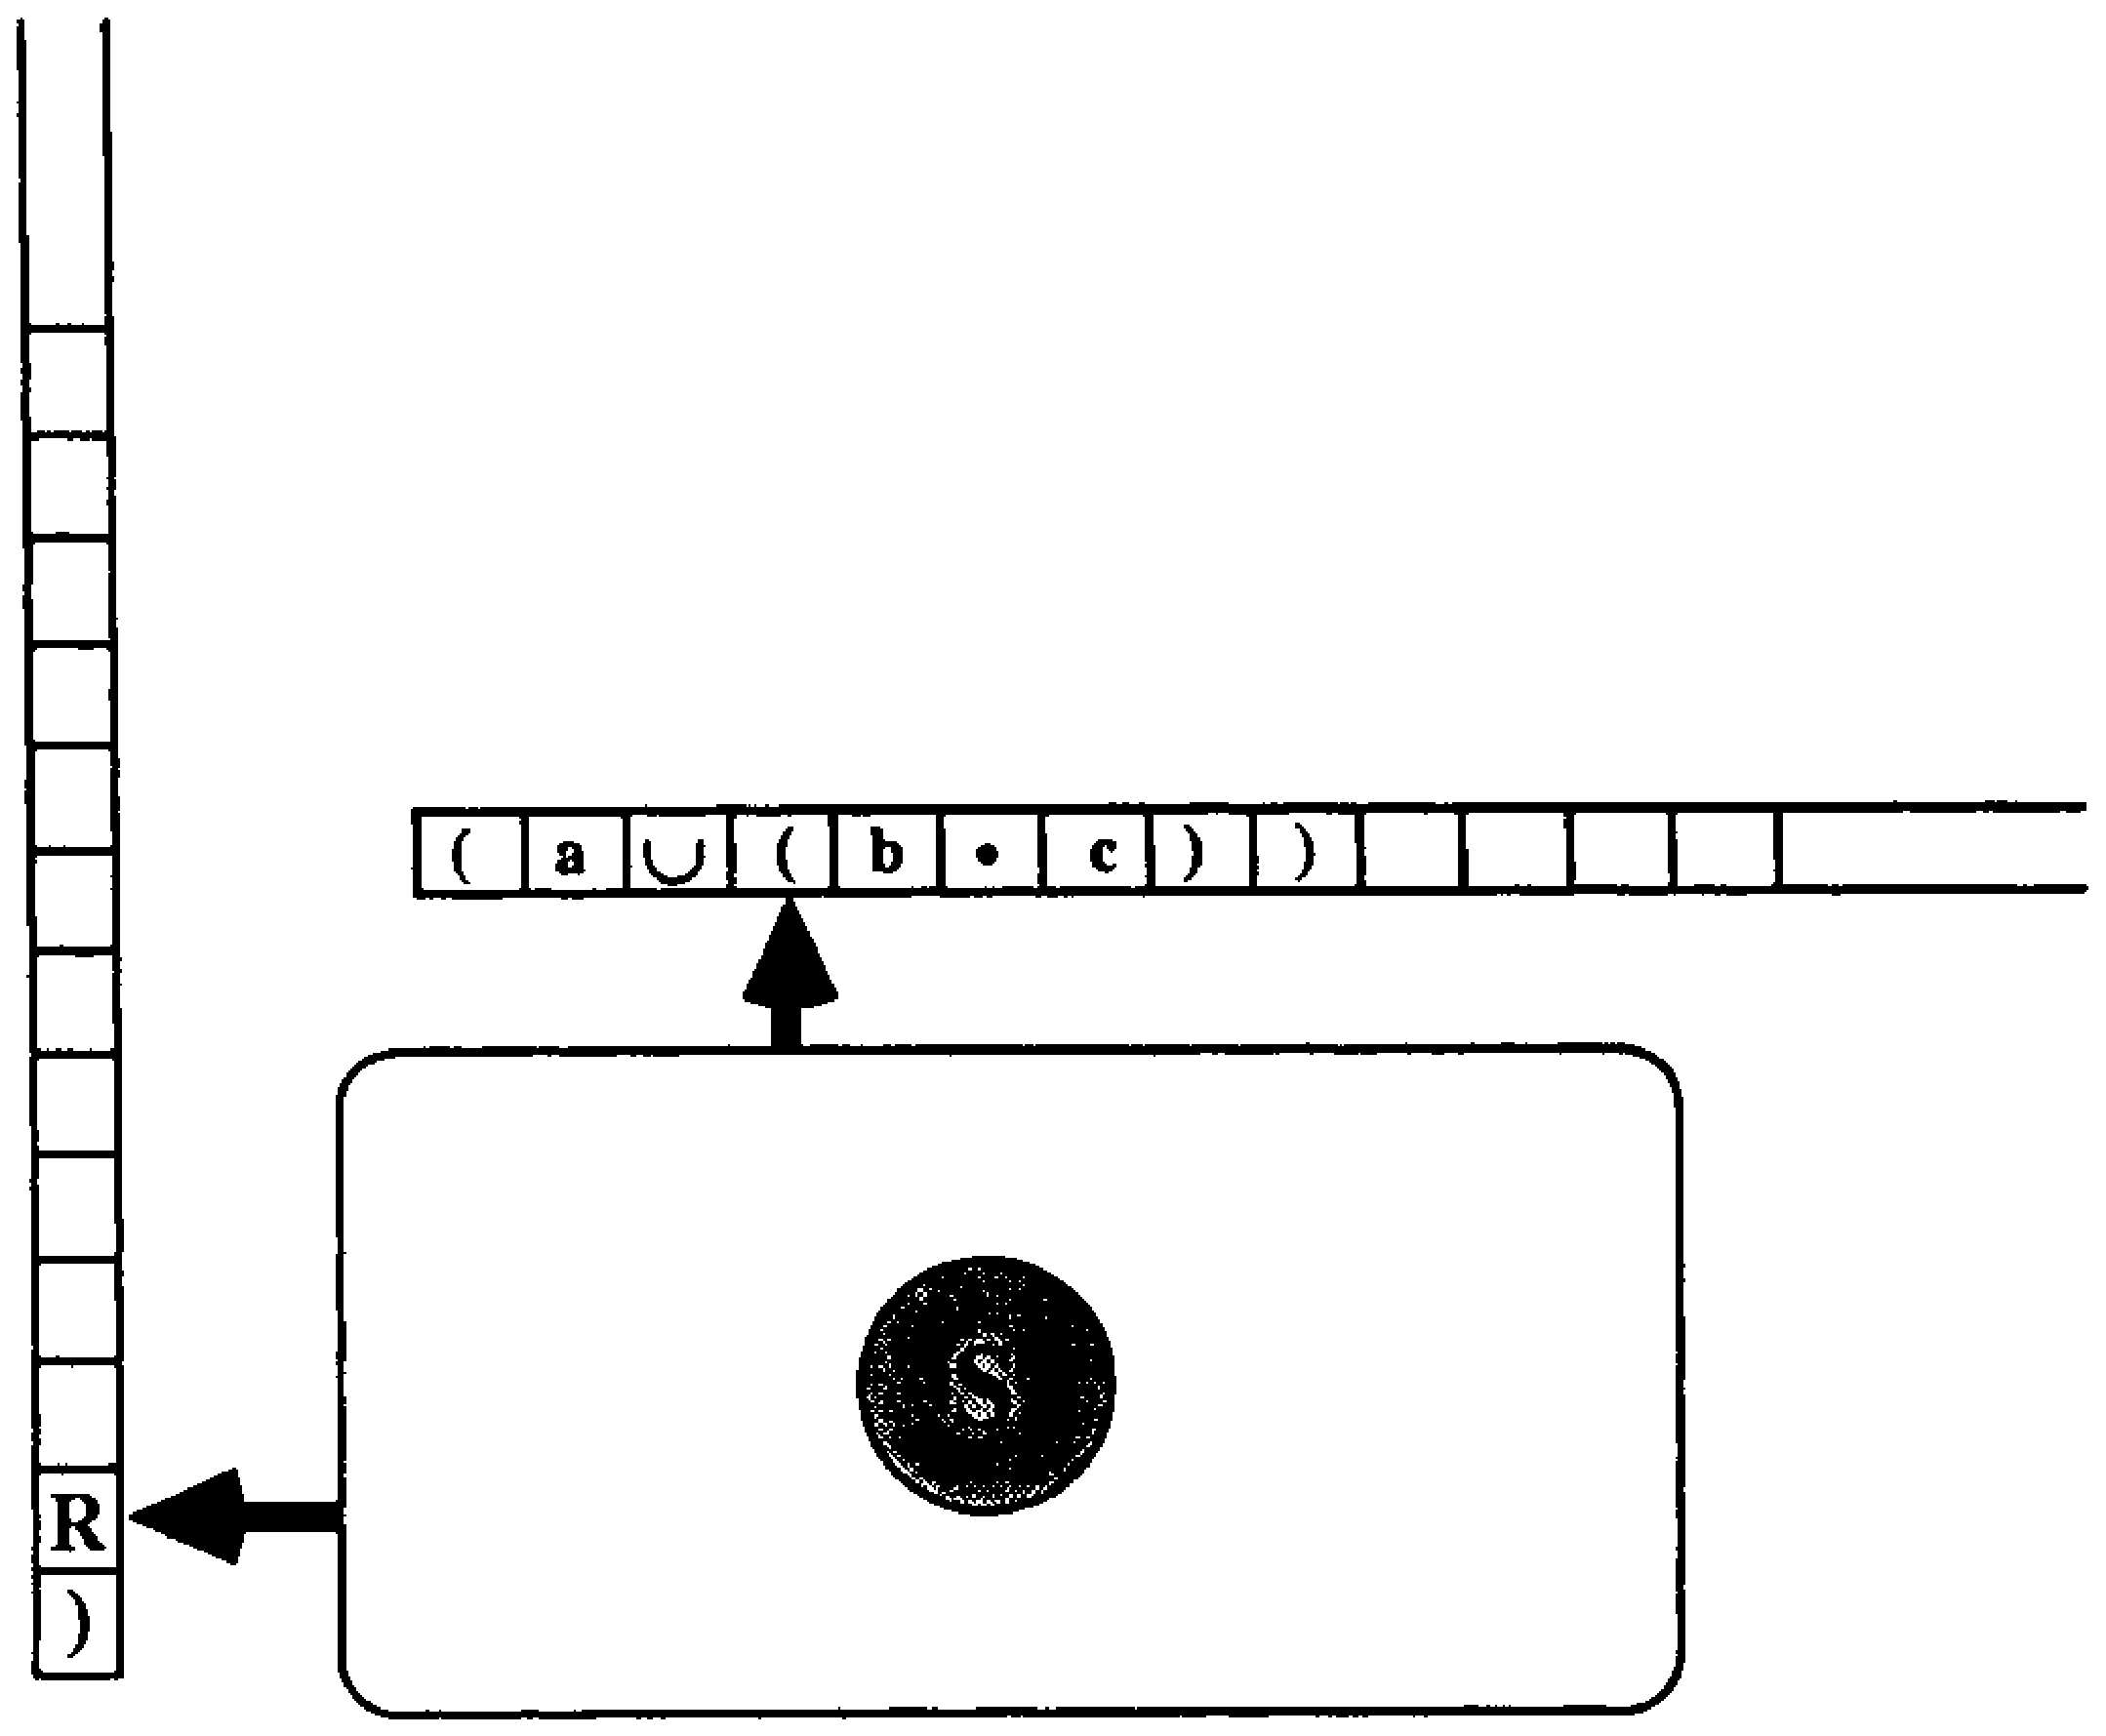
\epsfig{figure=ToFAfigures/fig10-5d.eps,height=2.0in}}
\caption{Walkthrough of the pushdown automaton discussed in Example 10.7}\label{fig-10.5d}
\end{figure}

% Figure 10.5e
\begin{figure}
\centerline{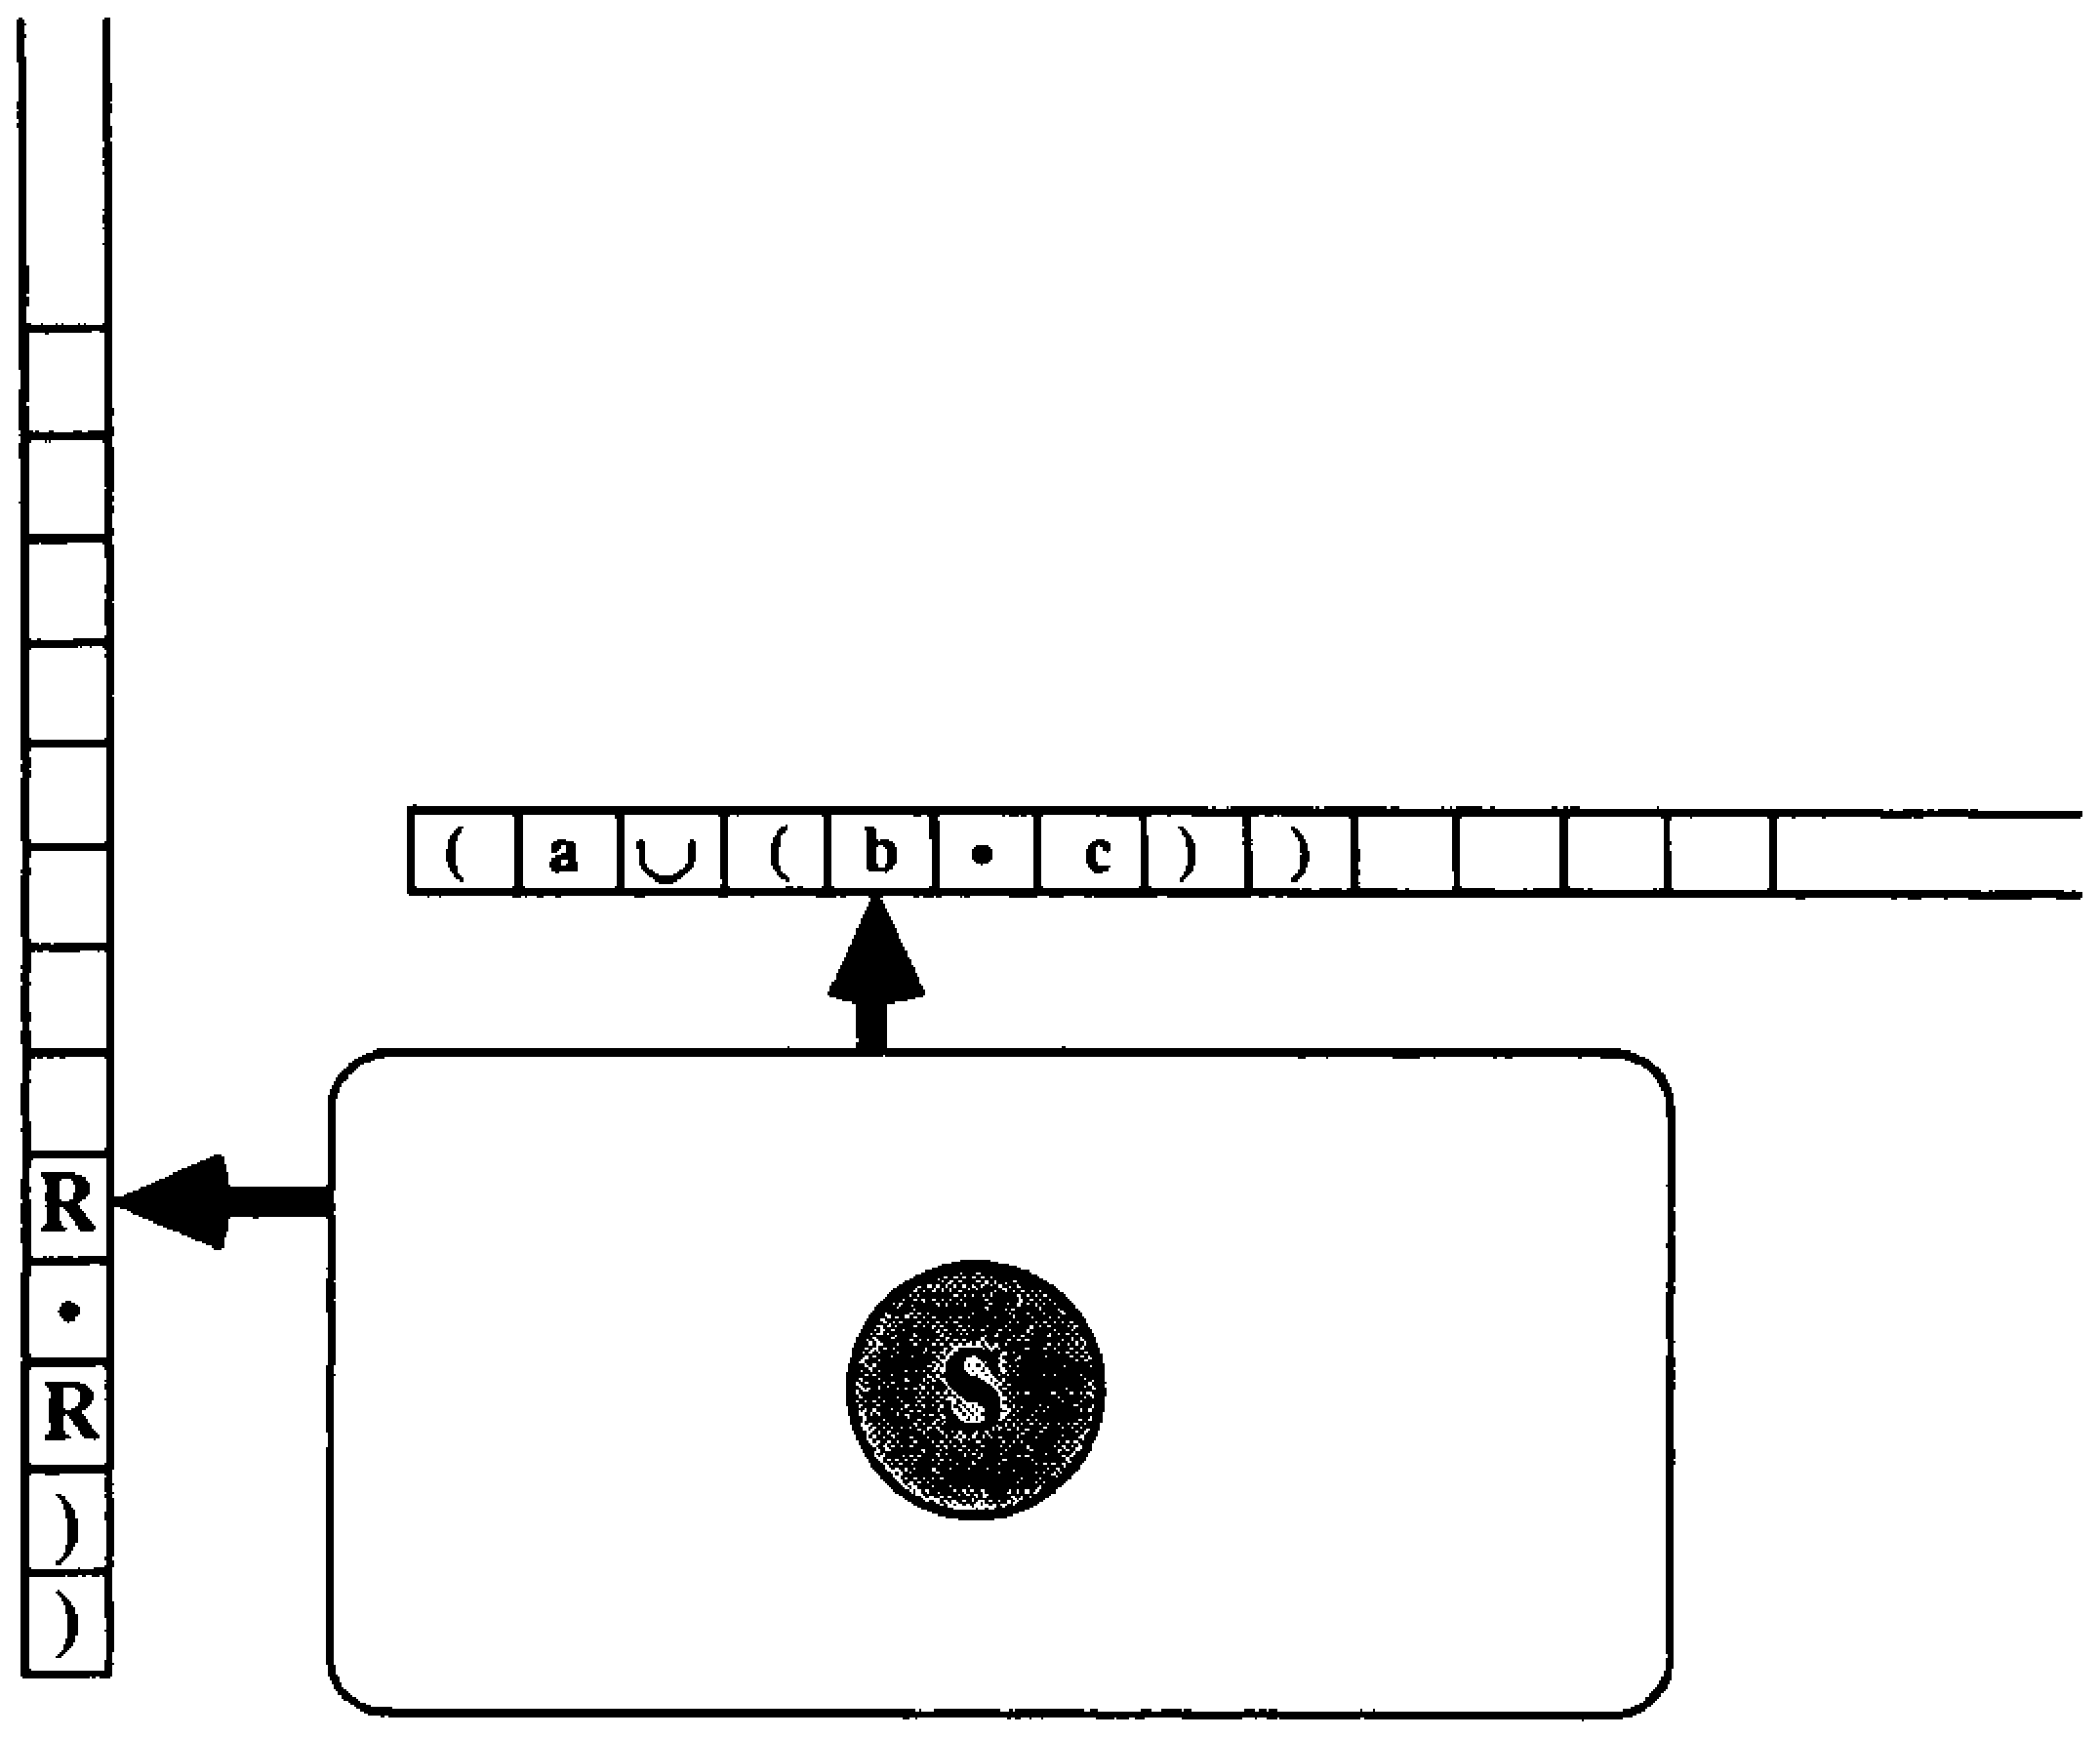
\epsfig{figure=ToFAfigures/fig10-5e.eps,height=2.0in}}
\caption{Walkthrough of the pushdown automaton discussed in Example 10.7}\label{fig-10.5e}
\end{figure}

% Figure 10.5f
\begin{figure}
\centerline{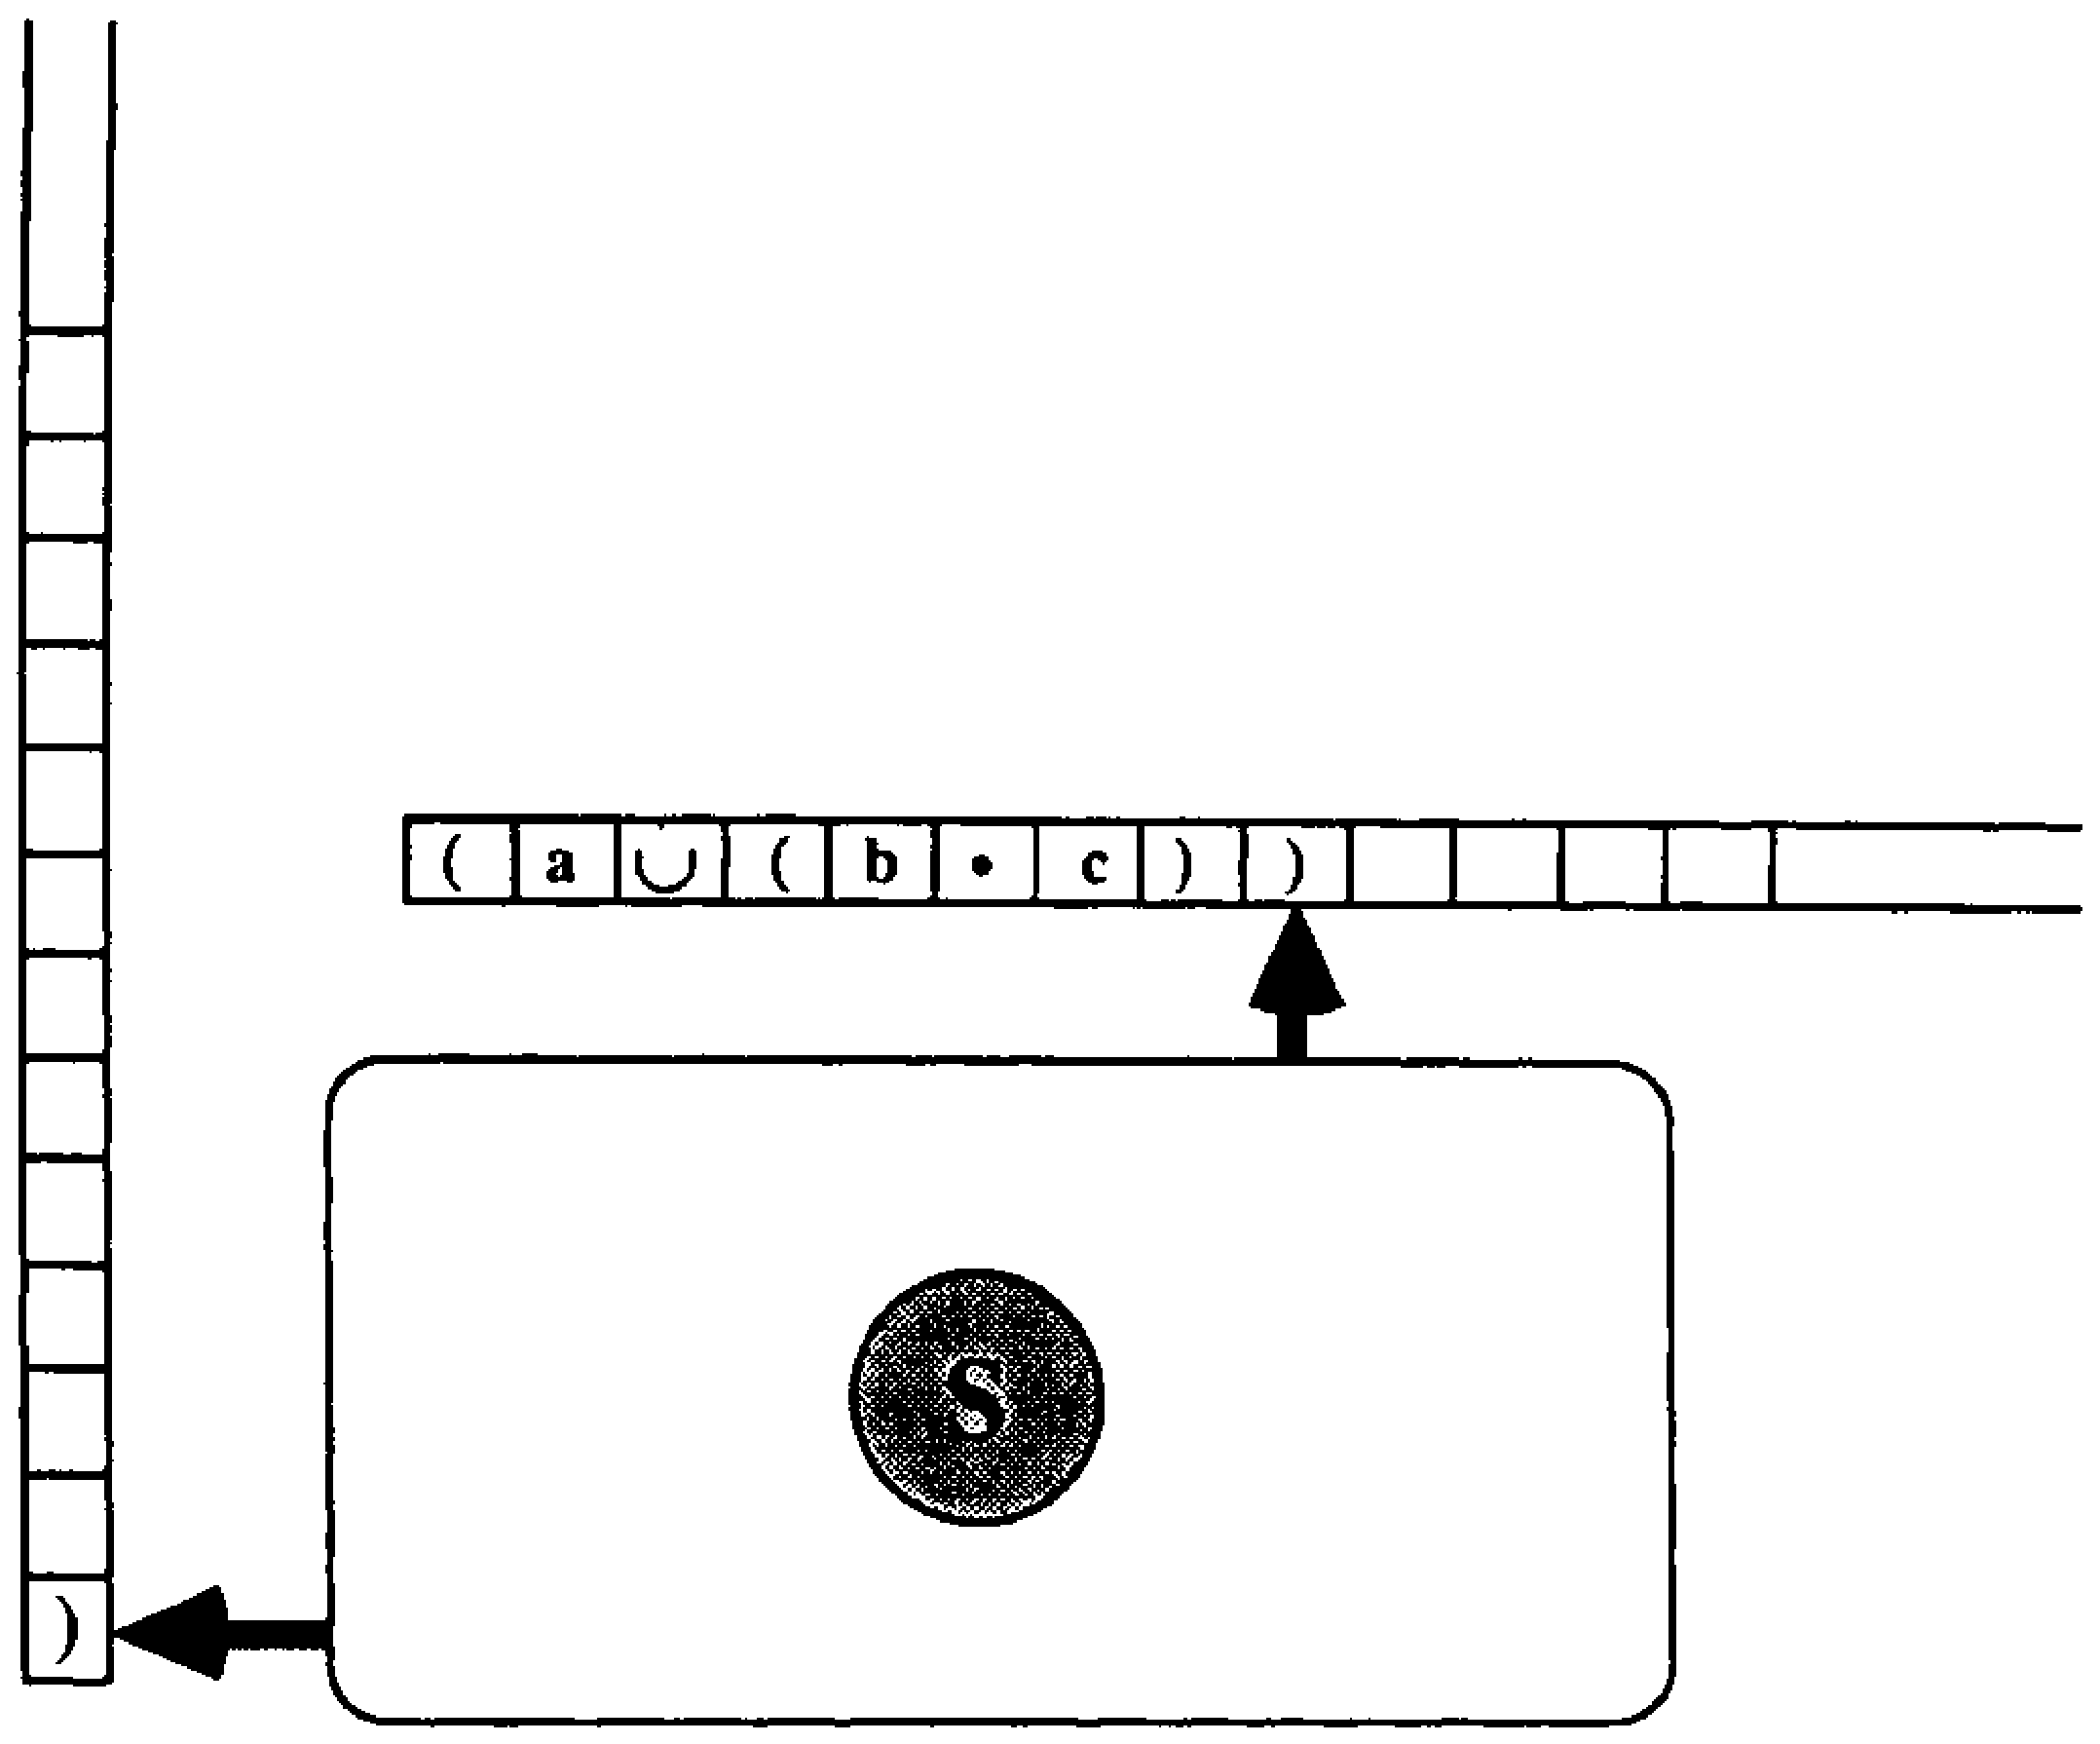
\epsfig{figure=ToFAfigures/fig10-5f.eps,height=2.0in}}
\caption{Walkthrough of the pushdown automaton discussed in Example 10.7}\label{fig-10.5f}
\end{figure}
\setcounter{figure}{5}                        %nasty kluge
\renewcommand{\thefigure}{\arabic{chapter}.\arabic{figure}}

% Theorem 10.2
\begin{thm}\label{thm-10.2}
Given any alphabet $\Sigma$, $\CSIG\subseteq\PSIG$. In particular, for any
context-free grammar $G$, there is a pushdown automaton that accepts (via empty
stack) the language generated by $G$.

\emph{Proof.} Let $G'$ be any context-free grammar. Theorem \ref{thm-9.6} guarantees that
there is a pure Greibach normal form grammar $G=\langle\Omega,\Sigma,S,P\rangle$
for which $L(G)=L(G')-\{\lambda\}$. If $\lambda\notin L(G')$, the PDA $P_G$ from
Definition \ref{dfn-10.6} can be used directly. If $\lambda\in L(G')$, then there is a
Greibach normal form grammar
\[ G''=\langle\Omega\cup\{Z\},\Sigma,Z,P\cup\{Z\rightarrow S,Z\rightarrow\lambda
	\}\rangle, \]
which generates $L(G')$, and the state transition function for $L(G')$ should
then include the move $\delta_G(s,\lambda,Z)=\{\langle s,S\rangle,\langle s,
\lambda\rangle\}$ to reflect the two $Z$-rules. The bottom of the stack symbol
would then be $Z$, the new start symbol.

In either case, induction on the number of moves in a sequence will show that\\
$(\forall x\in\Sigma^*)(\forall\beta\in(\Sigma\cup\Omega)^*)(\langle s,x,S
\rangle\Dvdash\langle s,\lambda,\beta\rangle  \ \ \  \Leftrightarrow\ \ \ S\ \DRightarrow x\beta$ as a
leftmost derivation).\\Note that $x\beta$ is likely to be a sentential form that
still contains nonterminals. The words $x$ that result in an empty stack ($\beta
=\lambda$) will then be exactly those words that produce an entire string of
terminal symbols from the start symbol $S$ (or $Z$ in the case where the grammar
contains the two special $Z$-rules). In other words, $L(G')=\Lambda(P_G)$.
\end{thm}

Given a context-free grammar, the definition of an equivalent PDA is easy once
an appropriate GNF grammar is in hand. In Example 10.6, the grammar was already
in Greibach normal form. To find a PDA for the grammar in Chapters \ref{ch-8} and \ref{ch-9} that
generates regular expressions, the grammar
\[ \langle\{R\},\{\pmb{a},\pmb{b},\pmb{c},\pmb{(},\pmb{)},\pmb{\epsilon},
	\pmb{\emptyset},\pmb{\cup},\pmb{\cdot},\pmb{^*}\},R,\{R\rightarrow
	\pmb{a}|\pmb{b}|\pmb{c}|\pmb{\epsilon}|\pmb{\emptyset}|\pmb{(}R
	\pmb{\cdot}R\pmb{)}|\pmb{(}R\pmb{\cup}R\pmb{)}|R\pmb{^*}\}\rangle \]
would have to be converted to Greibach normal form. The offending left-recursive
production $R\rightarrow R\pmb{^*}$ would have to be replaced, resulting in an
extra nonterminal and about three times as many productions. The definition of
the PDA for this grammar would be correspondingly more complex (see the
exercises).

Since every context-free language can be represented by a pushdown automaton
with only one state, one might suspect that more complex PDAs with extra states
may be able to define languages that are more complex than those in \CSIG. It
turns out that extra states yield no more cognitive power; the information
stored within the finite-state control can effectively be stored on the stack
tape. This will follow from the fact that the converse of Theorem \ref{thm-10.2}, that
context-free grammars have equivalent pushdown automata, is also true.

Defining a pushdown automaton based on a context-free grammar is not as elegant
as the construction presented in Definition \ref{dfn-10.6}, but the idea is to have the
leftmost derivations in the grammar correspond to successful move sequences in
the PDA.

% Definition 10.7
\begin{dfn}\label{dfn-10.7}
Let $P=\langle\Sigma,\Gamma,S,s_0,\delta,B,\emptyset\rangle$ be a pushdown
automaton. Define the grammar $G_P=\langle\Omega,\Sigma,Z,P_P\rangle$, where
\[ \Omega=\{Z\}\cup\{A^{st}|\ A\in\Gamma,s,t\in S\} \]
and
\begin{center}\begin{tabular}{r@{ }c@{ }l}
$P_P$ & $=$ & $\{Z\rightarrow B^{s_0t}|\ t\in S\}\cup\{A^{sq}\rightarrow\pmb{a}A^{rt_1}_1
	A^{t_1t_2}_2A^{t_2t_3}_3\cdots A^{t_{m-1}t_m}_{m-1}A^{t_mq}_m|\ A\in\Gamma,
	\pmb{a}\in\Sigma\cup\{\lambda\},$ \\
&& $\langle r,A_1A_2\cdots A_m\rangle\in\delta(s,\pmb{a},A),s,q,r,t_1,t_2,\ldots,
	t_m\in S\}$ \\
&& $\cup\ \{A^{sr}\rightarrow\pmb{a}\ |\ s,r\in S,A\in\Gamma,\pmb{a}\in\Sigma\cup\{
	\lambda\},\langle r,\lambda\rangle\in\delta(s,\pmb{a},A)\}$
\end{tabular}\end{center}
\end{dfn}

Note that when $m=1$, the transition $\langle r,A_1\rangle\in\delta(s,\pmb{a},A)$
gives rise to a rule of the form $A^{sq}\rightarrow\pmb{a}A^{rq}_1$ for each
state $q\in S$.

\subsection*{Example 10.8}

Consider again the pushdown automaton from Example 10.4, defined by $P_2=\langle
\{\pmb{a},\pmb{b}\},\{S,C\},\{t\},t,\delta,S,\emptyset\rangle$, where $\delta$
is given by
\begin{center}\begin{tabular}{r@{ = }l}
$\delta(t,\pmb{a},S)$ & $\{\langle t,SC\rangle,\langle t,C\rangle\}$ \\
$\delta(t,\pmb{a},C)$ & $\{\ \ \}$ \\
$\delta(t,\pmb{b},S)$ & $\{\ \ \}$ \\
$\delta(t,\pmb{b},C)$ & $\{\langle t,\lambda\rangle\}$
\end{tabular}\end{center}
Since there is but one state and two stack symbols, the nonterminals for the
corresponding grammar $G_{P_2}$ are $\Omega=\{Z,S^{tt},C^{tt}\}$. $P_{P_2}$ can
be calculated as follows: $Z\rightarrow S^{tt}$ is the only rule arising from
the first criteria for productions. Since $\delta(t,\pmb{a},S)$ contains
$\langle t,SC\rangle$, a move that produces two stack symbols, $m=2$ and the
resulting production is $S^{tt}\rightarrow\pmb{a}S^{tt}C^{tt}$. The only other
rule due to the second criteria arises because $\delta(t,\pmb{a},S)$ contains
$\langle t,C\rangle$, which with $m=1$ yields $S^{tt}\rightarrow\pmb{a}C^{tt}$.
Finally, $\langle t,\lambda\rangle\in\delta(t,\pmb{b},C)$ causes $C^{tt}
\rightarrow\pmb{b}$ to be added to the production set. The resulting grammar is
therefore
\[ G_{P_2}=\langle\{Z,S^{tt},C^{tt}\},\{\pmb{a},\pmb{b}\},Z,\{Z\rightarrow
	S^{tt},S^{tt}\rightarrow\pmb{a}S^{tt}C^{tt},S^{tt}\rightarrow\pmb{a}
	C^{tt},C^{tt}\rightarrow\pmb{b}\}\rangle \]
and $G_{P_2}$ does indeed generate $\{\pmb{a}^n\pmb{b}^n|\ n \geq 1\}$ and is
therefore equivalent to $P_2$.

\subsection*{Example 10.9}

Now consider the pushdown automaton from Example 10.1, defined by
\[ P_1 = \langle\{\pmb{a},\pmb{b}\},\{A,B\},\{q,r\},q,\delta,B,\emptyset\rangle, \]
where the nonempty transitions were
\begin{center}\begin{tabular}{r@{ = }l}
$\delta(q,\pmb{a},B)$ & $\{\langle q,A\rangle\}$ \\
$\delta(q,\pmb{a},A)$ & $\{\langle q,AA\rangle\}$ \\
$\delta(q,\pmb{b},A)$ & $\{\langle r,\lambda\rangle\}$ \\
$\delta(r,\pmb{b},A)$ & $\{\langle r,\lambda\rangle\}$
\end{tabular}\end{center}
Since there are two stack symbols and two choices for each of the state
superscripts, the nonterminal set for the grammar $G_{P_1}$ is $\Gamma=\{Z,B^{qq},
B^{qr},B^{rq},B^{rr},A^{qq},A^{qr},A^{rq},A^{rr}\}$, although some of these will
turn out to be useless.

$P_{P_1}$ contains the $Z$-rules $Z\rightarrow B^{qq}$ and $Z\rightarrow B^{qr}$
from the first criteria for productions. The transition $\delta(q,\pmb{a},B) =
\{\langle q,A\rangle\}$ accounts for the productions $B^{qr}\rightarrow\pmb{a}
A^{qr}$ and $B^{qq}\rightarrow\pmb{a}A^{qq}$\!. $\delta(q,\pmb{a},A)=\{\langle q,
AA\rangle\}$ gives rise to the $A^{qq}$\!-rules $A^{qq}\rightarrow\pmb{a}A^{qq}\!\!
A^{qq}$ and $A^{qq}\rightarrow\pmb{a}A^{qr}\!\!\!A^{rq}$, as well as $A^{qr}$\!-rules
$A^{qr}\rightarrow\pmb{a}A^{qq}\!\!A^{qr}$ and $A^{qr}\rightarrow\pmb{a}A^{qr}\!\!A^{rr}$\!\!.
$\delta(q,\pmb{b},A)=\{\langle r,\lambda\rangle\}$ accounts for another
$A^{qr}$-rule, $A^{qr}\rightarrow\pmb{b}$. Finally, the transition $\delta(r,
\pmb{b},A)=\{\langle r,\lambda\rangle\}$ generates the only $A^{rr}$\!-rule,
$A^{rr}\rightarrow\pmb{b}$.

Note that some of the potential nonterminals ($B^{qr}\!,B^{rq}\!,B^{rr}$) are never
generated, and others ($A^{qq}\!,B^{qq}$) cannot produce terminal strings. The
resulting grammar, with useless items deleted, is given by
\[ G_{P_1}=\langle\{Z,B^{qr}\!\!,A^{qr}\!\!,A^{rr}\},\{\pmb{a},\pmb{b}\},Z,\{Z
	\rightarrow B^{qr}\!\!,B^{qr}\rightarrow\pmb{a}A^{qr}\!\!,A^{qr}\rightarrow
	\pmb{a}A^{qr}\!\!A^{rr}\!\!,A^{qr}\rightarrow\pmb{b},A^{rr}\rightarrow\pmb{b}\}
	\rangle \]
and $G_{P_1}$ generates the language $P_1$ recognizes: $\{\pmb{a}^n\pmb{b}^n|\ n
\geq 1\}$.

Notice that the move sequence
\begin{center}\begin{tabular}{r@{ $\vdash$ }l}
$\langle q,\pmb{aaabbb},B\rangle$ & $\langle q,\pmb{aabbb},A\rangle$ \\
& $\langle q,\pmb{abbb},AA\rangle$ \\
& $\langle q,\pmb{bbb},AAA\rangle$ \\
& $\langle r,\pmb{bb},AA\rangle$ \\
& $\langle r,\pmb{b},A\rangle$ \\
& $\langle r,\lambda,\lambda\rangle$
\end{tabular}\end{center}
corresponds to the leftmost derivation
\begin{center}\begin{tabular}{r@{ $\Rightarrow$ }l}
$Z\Rightarrow B^{qr}$ & $\pmb{a}A^{qr}$ \\
& $\pmb{aa}A^{qr}\!\!A^{rr}$ \\
& $\pmb{aaa}A^{qr}\!\!A^{rr}\!\!A^{rr}$ \\
& $\pmb{aaab}A^{rr}\!\!A^{rr}$ \\
& $\pmb{aaabb}A^{rr}$ \\
& $\pmb{aaabbb}$
\end{tabular}\end{center}

Note the relationship between the sequence of stack configurations and the
nonterminals in the corresponding sentential form. For example, when $\pmb{aaa}$
has been processed by $P_1$, $AAA$ is on the stack, and when the leftmost
derivation has produced $\pmb{aaa}$, the remaining nonterminals are also three
$A$-based symbols ($A^{qr}\!\!A^{rr}\!\!A^{rr}$). $A^{qr}$ denotes a nonterminal (which
corresponds to the stack symbol $A$) that will eventually produce a terminal
string as the stack shrinks below the current size during a sequence of
transitions that lead from state $q$ to state $r$. This finally happens in the
last of the following steps, where $\pmb{aaa}A^{qr}\!\!A^{rr}\!\!A^{rr}\ \DRightarrow
\pmb{aaabbb}$. $A^{rr}$\!, by contrast, denotes a nonterminal (again corresponding
to the stack symbol $A$) that will produce a terminal string as the stack
shrinks in size during transitions from state $r$ back to state $r$. In this
example, this occurs in the next to the last two steps. The initial stack symbol
position held by $B$ is finally vacated during a sequence of transitions from
$q$ to $r$, and hence $B^{qr}$ appears in the leftmost derivation. On the other
hand, it was not possible to vacate $B$'s position during a sequence of moves
from $q$ to $q$, so $B^{qq}$ consequently does not participate in significant
derivations.

The strong correspondence between profitable move sequences in $P$ and valid
leftmost derivations in $G_P$ forms the cornerstone of the following proof.

% Theorem 10.3
\begin{thm}\label{thm-10.3}
Given any alphabet $\Sigma$, $\PSIG\subseteq\CSIG$. In particular, for any
pushdown automaton $P$, there is a context-free grammar $G_P$ for which $L(G_P)
= \Lambda(P)$.

\emph{Proof.} Let $P=\langle\Sigma,\Gamma,S,s_0,\delta,B,\emptyset\rangle$ be a
pushdown automaton, and let $G_P$ be the grammar given in Definition \ref{dfn-10.7}. The
key to the proof is to show that all words accepted by empty stack in the PDA
$P$ can be generated by $G_P$ and that only such words can be generated by $G_P$.
That is, we wish to show that the automaton halts in some state $t$ with an
empty stack after processing the terminal string $x$ exactly when there is a
leftmost derivation of the form
\[ Z \Rightarrow A^{s_0t}\  \DRightarrow x \]
That is,
\[ (\forall x\in\Sigma^*)(Z\Rightarrow B^{s_0t}\ \DRightarrow x  \ \ \  \Leftrightarrow\ \ \  
	\langle s_0,x, B\rangle \Dvdash \langle t,\lambda,\lambda\rangle) \]
The desired conclusion, that $L(G_P) = \Lambda(P)$, will follow immediately from
this equivalence. The equivalence does not easily lend itself to proof by
induction on the length of $x$; indeed, to progress from the $m^{th}$ to the
$m+1^{st}$ step, a more general statement involving more of the nonterminals of
$G_P$ is needed. The following statement can be proved by induction on the
number of moves and leads to the desired conclusion when $s=s_0$ and $A=B$:
\[ (\forall x\in\Sigma^*)(\forall A\in\Gamma)(\forall s\in S)(\forall t\in S)
	(A^{st}\ \DRightarrow x \ \ \  \Leftrightarrow\ \ \  \langle s,x,A\rangle \Dvdash
	\langle t,\lambda,\lambda\rangle) \]
The resulting grammar will then generate $\Lambda(P)$, but $G_P$ may not be a
strict context-free grammar; $\lambda$-moves may result in some productions of
the form $A^{sr}\rightarrow\lambda$, which will then have to be ``removed,'' as
specified by Exercise 9.16.
\end{thm}

Thus, $\PSIG=\CSIG$. Furthermore, only one state in a PDA is truly necessary, as
noted in the following corollary. In essence, this means that for PDAs that
accept by empty stack, any state information can be effectively encoded with the
information on the stack.

% Corollary 10.1
\begin{cor}\label{cor-10.1}
For every PDA $P$ that accepts via empty stack, there is an equivalent one-state
PDA $P'$ that also accepts via empty stack.

\emph{Proof.} Let $P$ be a PDA that accepts via empty stack. Let $P'=P_{G_P}$.
That is, from the original PDA $P$, find the corresponding context-free grammar
$G_P$. By Theorem \ref{thm-10.3}, this is equivalent to $P$. However, by Theorem \ref{thm-10.2}, the
grammar $G_P$ has an equivalent one-state PDA, which must also be equivalent to
$P$.
\end{cor}

Unlike the pushdown automata discussed in this section, PDAs that accept via
final state cannot always make do with a single state. As the exercises will
make clear, at least one final and one nonfinal state are typically necessary. Unlike
DFAs, PDAs with only one state \emph{can} accept some nontrivial languages, since
selected words can be rejected because there is no appropriate move sequence.
However, a single final state and a single nonfinal state
\emph{are} sufficient for full generality, as
shown in the following section.

\section{Equivalence Of Acceptance By Final State and Empty Stack}\label{sec-10.3}

In this section, we explore the ramifications of accepting words according to
the criteria that a final state can be reached after processing all the letters
on the input tape, rather than the criteria that the stack is emptied. Theorem
\ref{thm-10.4} will show that any language that can be accepted via empty stack can also
be accepted via final state. In terms of Definition \ref{dfn-10.5}, this means that
$\PSIG\subseteq\FSIG$. Since $\PSIG=\CSIG$, this means that every context-free
language can be accepted by a PDA via final state. Theorem \ref{thm-10.5} ensures that no
``new'' languages can be produced by pushdown automata that accept via final
state; $\FSIG\subseteq\PSIG$, and so $\FSIG=\PSIG=\CSIG$.

As in the last section, the key to the correspondence is the definition of an
appropriate translation from one finite representation to another. We first
consider a scheme for modifying a PDA so that the new device can transfer to a
final state whenever the old device was capable of emptying its stack. To do
this, we need to place a ``buffer'' symbol at the bottom of the stack, which will
appear when the original automaton would have emptied its stack. The new machine
operates in almost the same fashion as the original automaton; the differences
amount to an additional transition at the start of operation to install the new
buffer symbol and an extra move at the end of operation to transfer to the (new)
final state.

% Theorem 10.4
\begin{thm}\label{thm-10.4}\index{equivalent!PDAs}
Every pushdown automaton $P$ that accepts via empty stack has an equivalent
two-state pushdown automaton $P_{\!\!f}$ that accepts via final state.

\emph{Proof.} Corollary \ref{cor-10.1} guaranteed that every pushdown automaton that
accepts via empty stack has an equivalent one-state pushdown automaton that also
accepts via empty stack. Without loss of generality, we may therefore assume
that $P=\langle\Sigma,\Gamma,\{s\},s,\delta,B,\emptyset\rangle$. Define $P_{\!\!f}$ by
choosing a new state $f$ and two new stack symbols $Y$ and $Z$ such that $Y,Z
\notin \Gamma$, and let $P_{\!\!f} = \langle\Sigma,\Gamma\cup\{Y,Z\},\{s,f\},s,
\delta_{\!\!f},Z,\{f\}\rangle$, where $\delta_{\!\!f}$ is defined by:
\begin{enumerate}
\item $\delta_{\!\!f}(s,\lambda,Z) = \{\langle s,BY\rangle\}$
\item $(\forall\pmb{a}\in\Sigma)(\forall A\in\Gamma)(\delta_{\!\!f}(s,\pmb{a},A) =
	\delta(s,\pmb{a},A))$
\item $(\forall A\in\Gamma)(\delta_{\!\!f}(s,\lambda,A)=\delta(s,\lambda,A))$
\item $\delta_{\!\!f}(s,\lambda,Y)=\{\langle f,Y\rangle\}$
\item $(\forall\pmb{a}\in\Sigma)(\delta_{\!\!f}(s,\pmb{a},Z) = \{\ \ \} \wedge
	\delta_{\!\!f}(s,\pmb{a},Y) = \{\ \ \})$
\item $(\forall\pmb{a}\in\Sigma\cup\{\lambda\})(\forall A\in\Gamma\cup\{Y,Z\})
	(\delta_{\!\!f}(f,\pmb{a},A) = \{\ \ \})$
\end{enumerate}

Notice that rules 2 and 3 imply that, while the original stack symbols appear on
the stack, the machine moves exactly as the original PDA. Rules 5 and 6 indicate
that no letters can be consumed while there is a $Y$ or $Z$ on the stack, and no
moves are possible once the final state $f$ is reached. Since the bottom of the
stack symbol is now the new letter $Z$, rule 1 is the only rule that initially
applies. Its application results in a configuration very much like that of the
old PDA, with the symbol $Y$ underneath the old bottom of the stack symbol $B$.
$P_{\!\!f}$ now simulates $P$ until the $Y$ is uncovered (that is, until a point is
reached in which the old PDA would have emptied its stack). In such cases (and
only in such cases), rule 4 applies, and control can be transferred to the final
state $f$, and $P_{\!\!f}$ must then halt.

By inducting on the number of moves in a sequence, it can be shown for any
$\alpha$, $\beta\in\Gamma^*$ that
\[ (\forall x,y\in\Sigma^*)(\langle s,xy,\alpha\rangle\Dvdash \langle s,y,\beta\rangle
	\text{ in }P \Leftrightarrow \langle s,xy,\alpha Y\rangle \Dvdash \langle s,y,\beta Y\rangle
	\text{ in }P_{\!\!f}) \]
From this, with $y = \beta = \lambda$ and $\alpha = B$, it follows that

\[ (\forall x\in\Sigma^*)(\langle s,x,B\rangle\Dvdash\langle s,\lambda,\lambda\rangle
	\text{ in }P\Leftrightarrow\langle s,x,BY\rangle\Dvdash\langle s,\lambda,Y\rangle\text{ in }P_{\!\!f})\]
Consequently, since $\delta_{\!\!f}(s,\lambda,Z)=\{\langle s,BY\rangle\}$ and
$\delta_{\!\!f}(s,\lambda,Y)=\{\langle f,Y\rangle\}$,
\[ (\forall x\in\Sigma^*)(\langle s,x,B\rangle\Dvdash \langle s,\lambda,\lambda\rangle\text{ in }P
	\Leftrightarrow\langle s,x,Z\rangle\Dvdash\langle f,\lambda,Y\rangle\text{ in }P_{\!\!f})\]
which implies that $(\forall x\in\Sigma^*)(x\in\Lambda(P)\Leftrightarrow x\in
L(P_{\!\!f}))$, as was to be proved.
\end{thm}

Thus, every language which is $\Lambda(P)$ for some PDA can be recognized by a
PDA that accepts via final state, and this PDA need only employ one final and
one nonfinal state. Thus, $\PSIG\subseteq\FSIG$. One might conjecture that
\FSIG, might actually be larger than \PSIG, since some added capability might
arise if more than two states are used in a pushdown automaton that accepts via
final state. This is not the case, as demonstrated by the following theorem.
Once again, the information stored in the finite control can effectively be
transferred to the stack; only one final and one nonfinal state are needed to
accept any context-free language via final state, and context-free languages are
the only type accepted via final state.

% Theorem 10.5
\begin{thm}\label{thm-10.5}\index{equivalent!PDAs}
Every pushdown automaton $P$ that accepts via final state has an equivalent
pushdown automaton $P_{\lambda}$ that accepts via empty stack.

\emph{Proof.} Assume that $P=\langle\Sigma,\Gamma,S,s_0,\delta,B,F\rangle$.
Define $P_{\lambda}$ by choosing new stack symbols $Y$ and $Z$ such that $Y,Z
\notin\Gamma$ and a new state $e$ such that $e \notin S$, and let $P_{\lambda}=
\langle\Sigma,\Gamma\cup\{Y,Z\},S\cup\{e\},s_0,\delta_{\lambda},Z,\emptyset
\rangle$, where $\delta_{\lambda}$ is defined by:
\begin{enumerate}
\item $\delta_{\lambda}(s_0,\lambda,Z) = \{\langle s_0,BY\rangle\}$
\item $(\forall a\in\Sigma)(\forall A\in\Gamma)(\forall s\in S)(\delta_{\lambda}
	(s,\pmb{a},A) = \delta(s,\pmb{a},A))$
\item $(\forall A\in\Gamma)(\forall s\in S-F)(\delta_{\lambda}(s,\lambda,A) =
	\delta(s,\lambda,A))$
\item $(\forall A\in\Gamma)(\forall f\in F)(\delta_{\lambda}(f,\lambda,A)
	=\delta(f,\lambda,A)\cup\{\langle e,\lambda\rangle\})$
\item $(\forall A\in\Gamma)(\delta_{\lambda}(e,\lambda,A) = \{\langle e,\lambda
	\rangle\})$
\item $\delta_{\lambda}(e,\lambda,Y) = \{\langle e,\lambda\rangle\}$
\end{enumerate}

The first rule guards against $P_{\lambda}$ inappropriately accepting if $P$
simply empties its stack (by padding the stack with the new stack symbol $Y$).
The intent of rules 2 through 4 is to arrange for $P_{\lambda}$ to simulate the
moves of $P$ and allow $P_{\lambda}$ to enter the state $e$ when final states
can be reached. The state $e$ does not allow any further symbols to be processed,
but does allow the stack contents (including the new buffer symbol) to be
emptied via rules 5 and 6. Thus, $P_{\lambda}$ has a sequence of moves for input
$x$ that empties the stack exactly when $P$ has a sequence of moves that leads
to a final state.

By inducting on the number of moves in a sequence, it can be shown for any
$\alpha,\beta\in\Gamma^*$ that
\[ (\forall x,y\in\Sigma^*)(\forall s,t\in S)(\langle s,xy,\alpha\rangle\Dvdash
	\langle t,y,\beta\rangle\text{ in }P \Leftrightarrow \langle s,xy,\alpha Y\rangle
	\Dvdash\langle t,y,\beta Y\rangle\text{ in }P_{\lambda}) \]
From this, with $y=\lambda,\ \alpha = B$, and $t\in F$, it follows that
\[ (\forall x,y\in\Sigma^*)(\forall t\in F)(\langle s_0,x,B\rangle\Dvdash\langle
	t,\lambda,\beta\rangle\text{ in }P\Leftrightarrow\langle s_0,x,BY\rangle
	\Dvdash\langle t,\lambda,\beta Y\rangle\text{ in }P_{\lambda}) \]
Consequently, since $\delta_{\lambda}(s_0,\lambda,Z)=\{\langle s_0, BY\rangle\}$
and $\delta_{\lambda}(t,\lambda,A)$ contains $\langle e,\lambda\rangle$, repeated application
of rules 5 and 6 implies
\[ (\forall x,y\in\Sigma^*)(\forall t\in F)(\langle s_0,x,B\rangle\Dvdash\langle
	t,\lambda,\beta\rangle\text{ in }P\Leftrightarrow\langle s_0,x,Z\rangle\Dvdash
	\langle t,\lambda,\lambda\rangle\text{ in }P_{\lambda}) \]
This shows that $(\forall x\in\Sigma^*)(x\in \Lambda(P_{\lambda})\Leftrightarrow
x\in L(P))$.
\end{thm}

Thus, $\FSIG\subseteq\PSIG$ and so $\FSIG=\PSIG=\CSIG$. Acceptance by final
state yields exactly the same class of languages as acceptance by empty stack.
This class of languages, described by these cognitive constructs, has been
encountered before and can be defined by the generative constructs which
comprise the context-free grammars. Note that since the type 3 languages are
contained in the type 2 languages, the portion of Theorem \ref{thm-10.1} dealing with
pushdown automata follows immediately from the results in this and the previous
section.

\section{Closure Properties and Deterministic Pushdown Automata}\label{sec-10.4}

Since the collection of languages recognized by pushdown automata is exactly the
collection of context-free languages, the results in Chapter \ref{ch-9} show that \PSIG\ 
is closed under substitution, homomorphism, union, concatenation, and \Index{Kleene
closure}. Results for context-free languages likewise imply that \PSIG\ is not
closed under complement or intersection.

It is hard to imagine how to find a method that would combine two context-free
grammars to produce a new context-free grammar that might accept the
intersection of the original languages. The constructs for regular expressions
and regular grammars likewise did not lend themselves to such methods, and yet
it \emph{was} possible to find appropriate constructs that \emph{did} represent intersections.
As presented in Chapter \ref{ch-5}, this was possible by turning to the cognitive
representation for this class of languages, the deterministic finite automata.
It is instructive to recall the technique that allowed two DFAs $A_1$ and $A_2$
to be combined to form a new DFA $A^\cap$ that accepts the intersection of the
languages accepted by the original devices and to see why this same method
cannot be adapted to pushdown automata.

The automaton $A^{\cap}$ used a \Index{cross product} of the states of $A_1$ and $A_2$
to simultaneously keep track of the progress of both DFAs through an appropriate
revamping of the state transition function. $A^{\cap}$ only accepted strings that
would have reached final states in both $A_1$ and $A_2$. Two pushdown automata
$P_1$ and $P_2$ might be combined into a new PDA $P^{\cap}$ using the cross-product
approach, but the transition function for this composite PDA cannot be reliably
defined. A problem arises since the $\delta$ function depends on the top stack
symbol, and it is impossible to keep track of both the original stacks through
any type of stack encoding, since the stack size of $P_1$ might be increasing
while the stack size of $P_2$ is decreasing. A device like the one depicted in
Figure \ref{fig-10.6} could be capable of recognizing the intersection of two context-free
languages, but such a machine is inherently more powerful than PDAs. The
language $\{\pmb{a}^n\pmb{b}^n\pmb{c}^n|\ n\geq 0\}$ is not context free, yet a
two-tape automata could recognize this set of words by storing the initial
$\pmb{a}$s on the first stack tape, match them against the incoming $\pmb{b}$s while
storing those $\pmb{b}$s on the second tape, and then matching the $\pmb{c}$s
against the $\pmb{b}$s on the second tape (see the exercises).

If one were to attempt to intersect a context-free language with a regular
language, one would expect the result to be context free, since the
corresponding cross-product construct would need only one tape. This is indeed
the case, as shown by the following theorem.

% Figure 10.6
\begin{figure}
\centerline{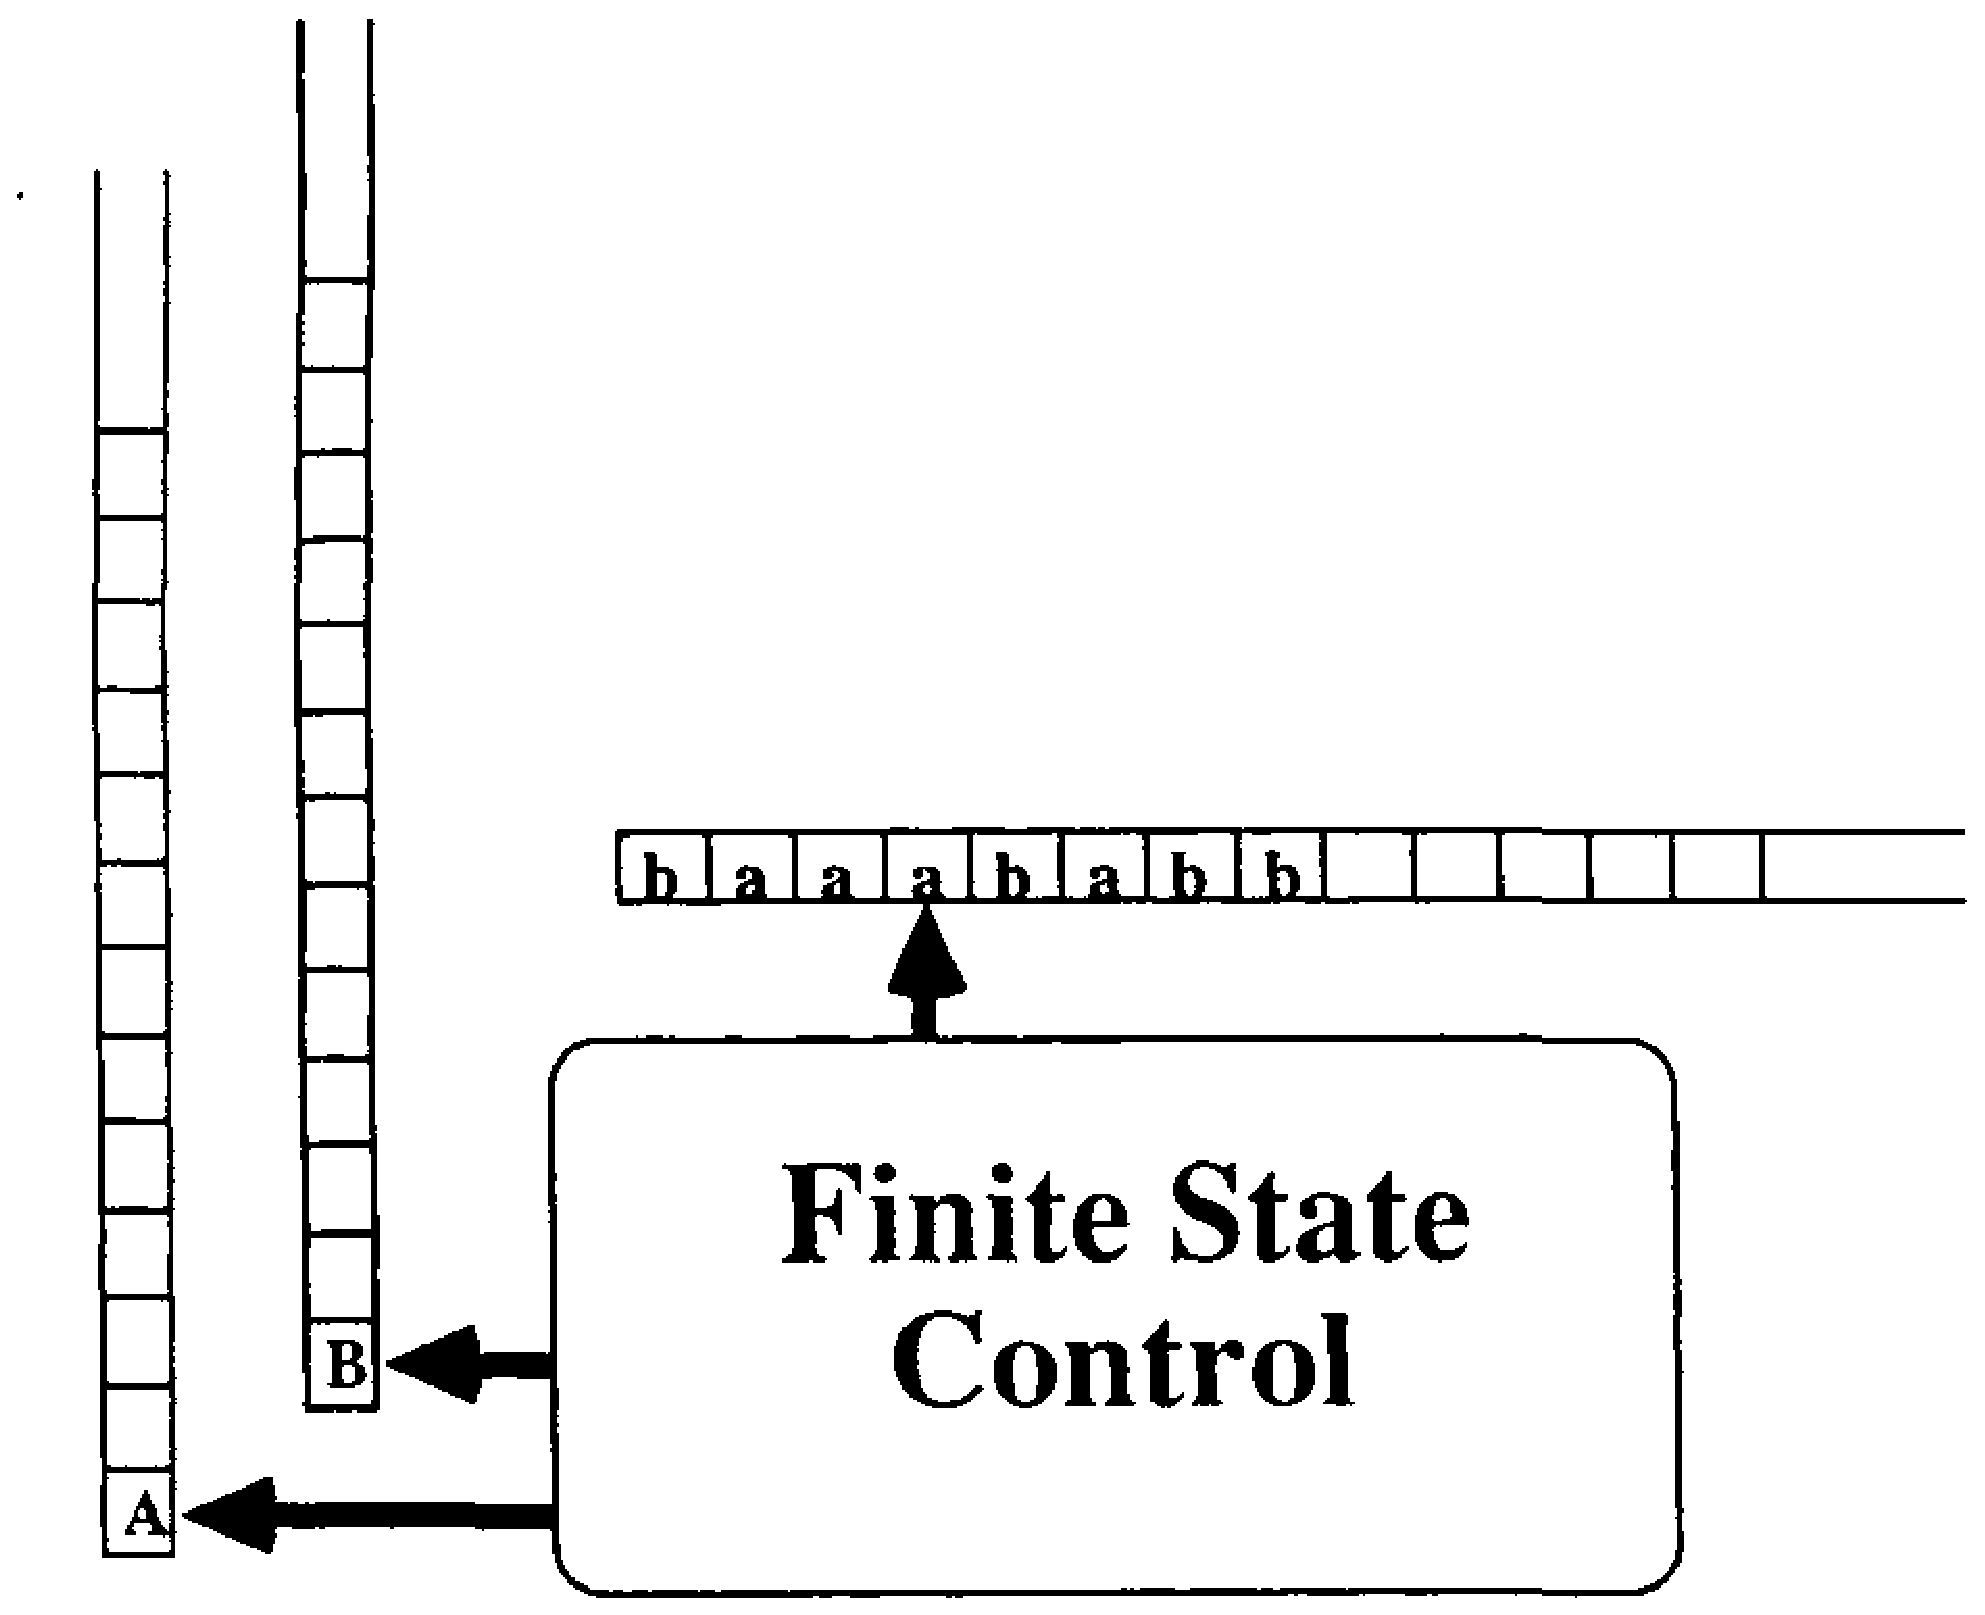
\epsfig{figure=ToFAfigures/fig10-6.eps,height=3.0in}}
\caption{A model of a ``pushdown automaton'' with two tapes}\label{fig-10.6}
\end{figure}

% Theorem 10.6
\begin{thm}\label{thm-10.6}
\CSIG\ is closed under intersection with a regular set. That is, if $L_1$ is
context free and $R_2 $is regular, $L_1\cap R_2$ is always context free.

\emph{Proof.} Let $L_1$ be a context-free language and let $R_2$ be a regular
set. Since $\CSIG=\FSIG$ there must be a PDA $P_1=\langle\Sigma,\Gamma_1,S_1,
s_{0_1},\delta_1,B_1,F_1\rangle$ for which $L_1=L(P_1)$. Let $A_2=\langle\Sigma,
S_2,s_{0_2},\delta_2,F_2\rangle$ be a DFA for which $R_2=L(A_2)$. Define
\[ P^{\cap} = \langle\Sigma,\Gamma_1,S_1\times S_2,\langle s_{0_1},s_{0_2}
	\rangle,\delta^{\cap},B_1,F_1\times F_2\rangle, \]
where $\delta^{\cap}$ is defined by:
\begin{enumerate}
\item $(\forall s_1\in S_1)(\forall s_2\in S_2)(\forall\pmb{a}\in\Sigma)(\forall
	A\in\Gamma_1)$ \\
	$(\delta^{\cap}(\langle s_1,s_2\rangle,\pmb{a},A)=\{\langle\langle t_1,
	t_2\rangle,\beta\rangle\ |\ \langle t_1,\beta\rangle\in\delta_1(s_1,\pmb{a},
	A)\wedge t_2=\delta_2(s_2,\pmb{a})\}).$
\item $(\forall s_1\in S_1)(\forall s_2\in S_2)(\forall A\in\Gamma_1)$ \\
	$(\delta^{\cap}(\langle s_1,s_2\rangle,\lambda,A)=\{\langle\langle t_1,
	t_2\rangle,\beta\rangle\ |\ \langle t_1,\beta\rangle\in\delta_1(s_1,\lambda,A)\wedge t_2
	=s_2\}).$
\end{enumerate}

As with the constructions in the previous sections, induction on the number of
moves exhibits the desired correspondence between the behaviors of the machines.
In particular, it can be shown for any $\alpha,\beta\in\Gamma^*$ that
\begin{center}\begin{tabular}{l}
$(\forall x\in\Sigma^*)(\forall s_1,t_1\in S_1)(\forall s_2,t_2\in S_2)
	(\langle\langle s_1,s_2\rangle,xy,\alpha\rangle\Dvdash\langle\langle
	t_1,t_2\rangle,y,\beta\rangle\text{ in }P_1\Leftrightarrow$ \\
$((\langle s_1,xy,	\alpha)\Dvdash\langle t_1,y,\beta\rangle\text{ in }
	P^{\cap})\wedge(t_2=\DBAR_2(s_2,x))))$
\end{tabular}\end{center}
From this, with $\alpha=B_1$, $s_1 = s_{0_1}$, $s_2 = s_{0_2}$ and the observation that $\langle t_1,t_2\rangle\in
F_1\times F_2$ $\Leftrightarrow$ $t_1\in F_1\wedge t_2\in F_2$, it follows that $(\forall x\in
\Sigma^*)(x\in L(P^{\cap})\Leftrightarrow (x\in L(P_1)\wedge x\in L(A_2)))$.
Therefore,
\[ L(P^{\cap})=L(P_1)\cap L(A_2)=L_1\cap R_2. \]
Since $P^{\cap}$ is a PDA accepting $L_1\cap R_2$, $L_1\cap R_2$ must be context
free.
\end{thm}

Closure properties such as this are quite useful in showing that certain
languages are not context free. Consider the set $L=\{x\in\{\pmb{a},\pmb{b},
\pmb{c}\}^*|\ \ |x|_{\pmb{a}} = |x|_{\pmb{b}} = |x|_{\pmb{c}}\}$. Since the letters
in a word can occur in any order, a pumping theorem proof is less
straight-forward than for the set $\{\pmb{a}^n\pmb{b}^n\pmb{c}^n|\ n\geq 0\}$.
However, if $L$ were context free, then $L\cap\pmb{a}^*\pmb{b}^*\pmb{c}^*$ would
also be context free (why?). But $L\cap\pmb{a}^*\pmb{b}^*\pmb{c}^*=\{\pmb{a}^n\pmb{b}^n
\pmb{c}^n|\ n\geq 0\}$, and thus $L$ cannot be context free. The exercises suggest
other occasions for which closure properties are useful in showing certain
languages are not context free.

For the machines discussed in the first portion of this text, it was seen that
nondeterminism did not add to the computing power of DFAs. In contrast, this
is not the case for pushdown automata. There are languages that can be accepted
by nondeterministic pushdown automata that cannot be accepted by any
deterministic pushdown automaton. The following is the broadest definition of
what can constitute a deterministic pushdown automaton.

% Definition 10.8
\begin{dfn}\label{dfn-10.8}
A\ \emph{\Index{deterministic pushdown automaton}} (\Index{DPDA}) is a pushdown
automaton\linebreak $P=\langle\Sigma,\Gamma,S,s_0,\delta,B,F\rangle$ with the following
restrictions on the state transition function $\delta$:
\begin{enumerate}
\item $(\forall\pmb{a}\in\Sigma)(\forall A\in\Gamma)(\forall s\in S)(\delta(s,
	\pmb{a},A)$ is empty or contains just one element).
\item $(\forall A\in\Gamma)(\forall s\in S)(\delta(s,\lambda,A)$ is empty or
	contains just one element).
\item $(\forall A\in\Gamma)(\forall s\in S)(\delta(s,\lambda,A)\not=\emptyset
	\Rightarrow (\forall\pmb{a}\in \Sigma)(\delta(s,\pmb{a},A)=\emptyset))$.
\end{enumerate}
\end{dfn}

Rule 1 states that, for a given input letter, deterministic pushdown automata
cannot have two different choices of destination states or two different choices
of strings to place on the stack. Rule 2 ensures that there is no choice of
$\lambda$-moves either. Furthermore, rule 3 guarantees that there will never be
a choice between a $\lambda$-move and a transition that consumes a letter;
states that have a $\lambda$-move can have \emph{only} that one move; no other
transitions of any type are allowed out of that state. Thus, for any string,
there is never any more than one path through the machine. Unlike deterministic
finite automata, deterministic pushdown automata may not always completely
process the strings in $\Sigma^*$; a given string may reach a state that has
no further valid moves, or a string may prematurely empty the stack. In each
case, the DPDA would halt without processing any further input (and reject the string).

\subsection*{Example 10.10}

The automaton $P_1$ in Example 10.1 was deterministic. The PDAs in Examples 10.4
and 10.5 were not deterministic. The automaton $P_G$ derived in Example 10.7 was
not deterministic because there were three possible choices of moves listed
for $\delta_G(s,\pmb{(}, R)$: $\{\langle s,R\cdot R\pmb{)}\rangle,\langle s,R
\cup R\pmb{)}\rangle,\langle s,R\pmb{)^*}\rangle\}$. These choices corresponded
to the three different operators that might have generated the open parenthesis.

Pushdown automata provide an appropriate mechanism for parsing sentences in
programming languages. The regular expression grammar in Example 10.7 is quite
similar to the arithmetic expression grammar that describes expressions in many
programming languages. Indeed, the transitions taken within the corresponding
PDA give an indication of which productions in the underlying grammar were used;
such information is of obvious use in compiler construction. A nondeterministic
pushdown automaton is at best a very inefficient tool for parsing; a DPDA is
much better suited to the task.

As mentioned in the proof of Theorem \ref{thm-10.2}, each leftmost derivation in $G$ has
a corresponding sequence of moves in $P_G$. If $G$ is ambiguous, then there is at
least one word with two distinct leftmost derivations, and hence if that word
appeared on the input tape of $P_G$, there would be two distinct move sequences
leading to acceptance. In this case, $P_G$ cannot possibly be deterministic. On
the other hand, if $P_G$ is nondeterministic, this does not mean that $G$ is
ambiguous, as demonstrated by Example 10.7. In parsing a string in that
automaton, it may not be immediately obvious which production to use (and hence
which transition to take), but for any string, there is at most only one correct
choice; each word has a unique parse tree and a unique leftmost derivation. The
grammar in Example 10.7 is not ambiguous, even though the corresponding PDA was
nondeterministic.

\subsection*{Example 10.11}

The following Greibach normal form grammar is similar to the one used to
construct the PDA in Example 10.7, but with the different operators paired with
unique delimiters. Let
\[ G=\langle\{R\},\{\pmb{a},\pmb{b},\pmb{c},\pmb{(},\pmb{)},\pmb{\{},\pmb{\}},
	\pmb{[},\pmb{]},\pmb{\epsilon},\pmb{\emptyset},\pmb{\cup},\pmb{\cdot},
	\pmb{^*}\},R,\{R\rightarrow\pmb{a}|\pmb{b}|\pmb{c}|\pmb{\epsilon}|
	\pmb{\emptyset}|\pmb{(}R\pmb{\cdot}R\pmb{)}|\pmb{[}R\pmb{\cup}R\pmb{]}|
	\pmb{\{}R\pmb{\}}^*\}\rangle. \]
The automaton $P_G$ is then
\[ \langle\{\pmb{a},\pmb{b},\pmb{c},\pmb{(},\pmb{)},\pmb{\{},\pmb{\}},\pmb{[},
	\pmb{]},\pmb{\epsilon},\pmb{\emptyset},\pmb{\cup},\pmb{\cdot},\pmb{^*}\},
	\{R,\pmb{a},\pmb{b},\pmb{c},\pmb{(},\pmb{)},\pmb{\{},\pmb{\}},\pmb{[},
	\pmb{]},\pmb{\epsilon},\pmb{\emptyset},\pmb{\cup},\pmb{\cdot},\pmb{^*}\},\{s\},s,
	\delta_G,R,\emptyset\rangle \]
where $\delta_G$ is comprised of the following nonempty transitions:
\begin{center}\begin{tabular}{r@{ = }l}
$\delta_G(s,\pmb{(},R)$ & $\{\langle s,R\pmb{\cdot}R\pmb{)}\rangle\}$ \\
$\delta_G(s,\pmb{[},R)$ & $\{\langle s,R\pmb{\cup}R\pmb{]}\rangle\}$ \\
$\delta_G(s,\pmb{\{},R)$ & $\{\langle s,R\pmb{\}^*}\rangle\}$ \\
$\delta_G(s,\pmb{a},R)$ & $\{\langle s,\lambda\rangle\}$ \\
$\delta_G(s,\pmb{b},R)$ & $\{\langle s,\lambda\rangle\}$ \\
$\delta_G(s,\pmb{c},R)$ & $\{\langle s,\lambda\rangle\}$ \\
$\delta_G(s,\pmb{\epsilon},R)$ & $\{\langle s,\lambda\rangle\}$ \\
$\delta_G(s,\pmb{\emptyset}, R)$ & $\{\langle s,\lambda\rangle\}$ \\
$\delta_G(s,\pmb{a},\pmb{a})$ & $\{\langle s,\lambda\rangle\}$ \\
$\delta_G(s,\pmb{b},\pmb{b})$ & $\{\langle s,\lambda\rangle\}$ \\
$\delta_G(s,\pmb{c},\pmb{c})$ & $\{\langle s,\lambda\rangle\}$ \\
$\delta_G(s,\pmb{\emptyset},\pmb{\emptyset})$ & $\{\langle s,\lambda\rangle\}$ \\
$\delta_G(s,\pmb{\epsilon},\pmb{\epsilon})$ & $\{\langle s,\lambda\rangle\}$ \\
$\delta_G(s,\pmb{\cup},\pmb{\cup})$ & $\{\langle s,\lambda\rangle\}$ \\
$\delta_G(s,\pmb{\cdot},\pmb{\cdot})$ & $\{\langle s,\lambda\rangle\}$ \\
$\delta_G(s,\pmb{^*},\pmb{^*})$ & $\{\langle s,\lambda\rangle\}$ \\
$\delta_G(s,\pmb{)},\pmb{)})$ & $\{\langle s,\lambda\rangle\}$ \\
$\delta_G(s,\pmb{]},\pmb{]})$ & $\{\langle s,\lambda\rangle\}$ \\
$\delta_G(s,\pmb{\}},\pmb{\}})$ & $\{\langle s,\lambda\rangle\}$ \\
$\delta_G(s,\pmb{(},\pmb{(})$ & $\{\langle s,\lambda\rangle\}$ \\
$\delta_G(s,\pmb{[},\pmb{[})$ & $\{\langle s,\lambda\rangle\}$ \\
$\delta_G(s,\pmb{\{},\pmb{\{})$ & $\{\langle s,\lambda\rangle\}$
\end{tabular}\end{center}

All other transitions are empty; that is, they are of the form $\delta_G(s,
\pmb{d},A) = \{\ \ \}$. The resulting PDA is clearly deterministic, since there
are no $\lambda$-moves and the other transitions are all singleton sets or are
empty. It is instructive to step through the transitions in $P_G$ for a string
such as $\pmb{[\{(a\cdot b)\}^*\cup c]}$. Upon encountering a delimiter while
scanning a prospective string, the parser would immediately know which operation
gave rise to that delimiter, and need not ``guess'' at which of the three
productions might have been applied. Note that $G$ was an LL0 grammar (as
defined in Section \ref{sec-9.2}), and the properties of $G$ resulted in $P_G$ being a
deterministic device. An efficient parser for this language follows immediately
from the specification of the grammar, whereas the grammar in Example 10.7 gave
rise to a nondeterministic device.

Programmers would not be inclined to tolerate remembering which delimiters
should be used in conjunction with the various operators, and hence programming
language designers take a slightly different approach to the problem. The
nondeterminism in Example 10.7 may only be an effect of the particular grammar
chosen and not inherent in the language itself. Note that the language
$\{\pmb{a}^n\pmb{b}^n|\ n\geq 1\}$ had a grammar that produced a nondeterministic
PDA (Example 10.4), but it also had a grammar that corresponded to a DPDA
(Example 10.1). In compiler construction, designers lean toward syntax that is
compatible with determinism, and they seek grammars for the language that
reflect that determinism.

\subsection*{Example 10.12}

Consider again the language discussed in Example 10.7, which can also be
expressed by the following grammar
\[ H = \langle\{S,T\},\{\pmb{a},\pmb{b},\pmb{c},\pmb{(},\pmb{)},\pmb{\epsilon},
	\pmb{\emptyset},\pmb{\cup},\pmb{\cdot},\pmb{^*}\},S,\{S\rightarrow\pmb{(}ST|
	\pmb{a}|\pmb{b}|\pmb{c}|\pmb{\epsilon}|\pmb{\emptyset},T\rightarrow
	\pmb{\cdot}S\pmb{)}|\pmb{\cup} S\pmb{)}|\pmb{)^*}\}\rangle \]
The automaton $P_H$ is then
\[ \langle\{\pmb{a},\pmb{b},\pmb{c},\pmb{(},\pmb{)},\pmb{\epsilon},
	\pmb{\emptyset},\pmb{\cup},\pmb{\cdot},\pmb{^*}\},\{S,T,\pmb{a},\pmb{b},
	\pmb{c},\pmb{(},\pmb{)},\pmb{\epsilon},\pmb{\emptyset},\pmb{\cup},
	\pmb{\cdot},\pmb{^*}\},\{t\},t,\delta_H,S,\emptyset\rangle \]
where each production of $H$ gives rise to the following transitions in
$\delta_H$:
\begin{center}\begin{tabular}{r@{ = }l}
$\delta_H(t,\pmb{(},S)$ & $\{\langle t,ST\rangle\}$ \\
$\delta_H(t,\pmb{a},S)$ & $\{\langle t,\lambda\rangle\}$ \\
$\delta_H(t,\pmb{b},S)$ & $\{\langle t,\lambda\rangle\}$ \\
$\delta_H(t,\pmb{c},S)$ & $\{\langle t,\lambda\rangle\}$ \\
$\delta_H(t,\pmb{\epsilon},S)$ & $\{\langle t,\lambda\rangle\}$ \\
$\delta_H(t,\pmb{\emptyset},S)$ & $\{\langle t,\lambda\rangle\}$ \\
$\delta_H(t,\pmb{\cdot},T)$ & $\{\langle t,S\pmb{)}\rangle\}$ \\
$\delta_H(t,\pmb{\cup},T)$ & $\{\langle t,S\pmb{)}\rangle\}$ \\
$\delta_H(t,\pmb{)},T)$ & $\{\langle t,\pmb{^*}\rangle\}$
\end{tabular}\end{center}
While the formal definition of $\delta_H$ specifies several productions of the
form $\delta_H(t,\pmb{d},\pmb{d})=\{\langle t,\lambda\rangle\}$, by observing
what can be put on the stack by the above productions, it is clear that the only
remaining useful transitions in $\delta_H$ are
\[ \delta_H(t,\pmb{^*},\pmb{^*})=\{\langle t,\lambda\rangle\} \]
and
\[ \delta_H(t,\pmb{)},\pmb{)})=\{\langle t,\lambda\rangle\} \]

Thus, even though the PDA $P_G$ in Example 10.7 turned out to be nondeterministic,
this was not a flaw in the language itself, since $P_H$ is an equivalent DPDA.
Notice that the grammar $G$ certainly appears to be more straightforward than
$H$. $G$ had fewer nonterminals and fewer productions, and it is a bit harder to
understand the relationships between the nonterminals of $H$. Nevertheless, the
LL0 grammar $H$ led to an efficient parser and G did not.

To take advantage of the resulting reduction in complexity, all major
programming languages are designed to be recognized by DPDAs. These constructs
naturally lead to a mechanical framework for syntactic analysis. In Example
10.12, the application of the production $T\rightarrow\pmb{\cup} S\pmb{)}$ [that is,
the use of the transition $\delta_H(t,\pmb{\cup},T)=\{\langle t,S\pmb{)}\rangle\}$\ ]
signifies that the previous expression and the expression to which $S$ will
expand are to be combined with the union operator. It should be easy to see that
a similar grammar and DPDA for arithmetic expressions (using $+,-,^*$, and $/$
rather than $\cup,\cdot$ and $^*$) would provide a guide for converting such
expressions into their equivalent machine code.

Deterministic pushdown automata have some surprising properties. Recall that
\CSIG\ was not closed under complementation, and since $\PSIG=\CSIG$, there
must be some PDAs that define languages whose complement cannot be recognized by
any PDA. However, it can be shown that any language accepted by a DPDA must have
a complement that can also be recognized by a DPDA. The construction used to
prove this statement, in which final and nonfinal states are interchanged in a
DPDA that accepts via final state, is similar to the approach used in Theorem
\ref{thm-5.1} for deterministic finite automata. It is useful to recall why it was crucial
in the proof of Theorem \ref{thm-5.1} to begin with a DFA when interchanging states,
rather than using an NDFA. Strings that have multiple paths in an NDFA that lead
to both final and nonfinal states would be accepted in the original automaton
and also in the machine with the states interchanged. Furthermore, some strings
may have no complete paths through the NDFA and be rejected in both the original
and new automata. The problem of multiple paths does not arise with DPDAs, since
by definition no choice of moves is allowed. However, strings that do not get
completely consumed would be rejected in both the original DPDA and the DPDA
with final and nonfinal states interchanged. Thus, the proof of closure under
complement for DPDAs is not as straightforward as for DFAs. There are three ways
an input string might not be completely consumed: the stack might empty
prematurely, there may be no transition available at some point, or there might
only be a cycle of $\lambda$-moves available that consumes no further input. The
exercises indicate that it is possible to avoid these problems by padding the
stack with a new bottom-of-the-stack symbol, and adding a ``garbage state'' to
which strings that are hopelessly stuck would transfer.

% Theorem 10.7
\begin{thm}\label{thm-10.7}
If $L$ is a language recognized by a deterministic pushdown automaton, then
$\sim\!\!L$ can also be recognized by a DPDA.

\emph{Proof.} See the exercises.
\end{thm}

% Definition 10.9
\begin{dfn}\label{dfn-10.9}\index{A @\ASIG \ (A-sigma )}
Given any alphabet $\Sigma$, let \ASIG\ represent the collection of all languages
recognized by deterministic pushdown automata. If $L\in\ASIG$, then $L$ is said
to be a \emph{\Index{deterministic context-free language}} (\Index{DCFL}).
\end{dfn}

Theorem \ref{thm-10.7} shows that unlike \PSIG, \ASIG is closed under complementation.
This divergent behavior has some immediate consequences, as stated below.

% Theorem 10.8
\begin{thm}\label{thm-10.8}
Let $\Sigma$ be an alphabet.
\begin{quote}
If \ $|\Sigma|=1$, then $\DSIG = \ASIG = \PSIG$. \\
If \ $|\Sigma|>1$, then \DSIG\ is properly contained in \ASIG, which is properly
contained in \PSIG.
\end{quote}

\emph{Proof.} For every alphabet $\Sigma$, examining the proof of Theorem \ref{thm-10.1}
shows that every finite automaton has an equivalent deterministic pushdown
automaton, and thus it is always true that $\DSIG\subseteq\ASIG$. Definition
\ref{dfn-10.7} implies that $\ASIG\subseteq\PSIG$. If $|\Sigma|=1$, then Theorem \ref{thm-9.15}
showed that $\DSIG = \CSIG\  ( = \PSIG)$, from which it follows that $\DSIG =
\ASIG = \PSIG$. If\, $|\Sigma|>1$, an example such as $\{\pmb{a}^n\pmb{b}^n|\,n\geq
1\}$ shows that \DSIG\ is properly contained in \ASIG\ (see the exercises).
Since $\mathfrak{P}_{\{\pmb{a},\pmb{b}\}}$ and $\cal{A}_{\{\pmb{a},
\pmb{b}\}}$ have different closure properties, they cannot represent the same
collection, and $\ASIG\subseteq\PSIG$ implies that the containment must be
proper.
\end{thm}

In the proof of Theorem \ref{thm-10.6}, it is easy to see that if $P_1$ is deterministic
then $P^{\cap}$ will be a DPDA, also. Hence \ASIG, like \PSIG, is closed under
intersection with a regular set. Also, the exercises show that both \ASIG\ and
\PSIG\ are closed under difference with a regular set. However, the closure
properties of \ASIG\ and \PSIG\  disagree in just about every other case. The
languages
\[ L_1 = \{\pmb{a}^n\pmb{b}^m|\ (n \geq 1)\wedge(n = m)\}\qquad\text{and}\qquad
	L_2 = \{\pmb{a}^n\pmb{b}^m|\ (n \geq 1)\wedge(n = 2m)\} \]
are both DCFLs, and yet $L_1\cup L_2 = \{\pmb{a}^n\pmb{b}^m|\ (n \geq 1)\wedge(n=
m \vee n = 2m)\}$ is not a DCFL (see the exercises). Thus, unlike \PSIG, \ASIG\ 
is not closed under union if $\Sigma$ is comprised of at least two symbols
(recall that since $\mathfrak{D}_{\{\pmb{a}\}} = \cal{A}_{\{\pmb{a}\}} =
\mathfrak{P}_{\{\pmb{a}\}}$, $\cal{A}_{\{\pmb{a}\}}$ would be closed under
union). If \ASIG\ was closed under intersection, then \ASIG\ would (by
De~Morgan's law) be closed under union, since it is closed under complement. Hence,
\ASIG\ cannot be closed under intersection.

The language $\{\pmb{c}^n\pmb{b}^m|\ (n \geq 1)\wedge(n=m)\}\cup\{\pmb{a}^n
\pmb{b}^m|\ (n \geq 1)\wedge(n=2m)\}$ is definitely a DCFL, and yet a simple
homomorphism can transform it into
\[ \{\pmb{a}^n\pmb{b}^m|\ (n\geq 1)\wedge((n=m)\vee(n=2m))\} \]
(see the exercises). Thus, \ASIG\ is not closed under homomorphism. Since
homomorphisms are special cases of substitutions, \ASIG\ is not closed under
substitution either. \ASIG\ is also the only collection of languages discussed
in this text that is not closed under reversal; $\{\pmb{ca}^n\pmb{b}^m|\ (n\geq 1)
\wedge(n=m)\}\cup\{\pmb{a}^n\pmb{b}^m|\ (n\geq 1)\wedge(n=2m)\}$ is a DCFL, but
$\{\pmb{b}^m\pmb{a}^n\pmb{c}\ |\ (n\geq 1)\wedge(n=m)\}\cup\{\pmb{b}^m\pmb{a}^n|\ (n
\geq 1)\wedge(n=2m)\}$ is not. These properties are summed up in the following
statements.

% Theorem 10.9
\begin{thm}\label{thm-10.9}
Given any alphabet $\Sigma$, \ASIG\ is closed under complement. \ASIG\ is also
closed under union, intersection, and difference \emph{with a regular set}. That
is, if $L_1$ is a DCFL and $R_2$ is a FAD language, then the following are
deterministic, context-free languages:
\begin{center}\begin{tabular}{c}
$\sim\!\!L_1$ \\
$L_1 \cap R_2$ \\
$L_1 \cup R_2$ \\
$L_1 - R_2$ \\
$R_2 - L_1$
\end{tabular}\end{center}

\emph{Proof.} The proof follows from the above discussion and theorems and the
exercises.
\end{thm}

% Lemma 10.1
\begin{lmm}\label{lmm-10.1}
Let $\Sigma$ be an alphabet comprised of at least two symbols. Then \ASIG\ is
not closed under union, intersection, concatenation, \Index{Kleene closure},
homomorphism, substitution, or reversal. That is, there are examples of
deterministic context-free languages $L_1$ and $L_2$, a homomorphism $h$, and a
substitution $s$ for which the following are not DCFLs:
\begin{center}\begin{tabular}{l}
$L_1 \cup L_2$ \\
$L_1 \cap L_2$ \\
$L_1 \cdot L_2$ \\
$L^*_1$ \\
$\overline{h}(L_1)$ \\
$\overline{s}(L_1)$ \\
$L^r_1$
\end{tabular}\end{center}

\emph{Proof.} The proof follows from the above discussion and theorems and the
exercises.
\end{lmm}

\subsection*{Example 10.13}

These closure properties can often be used to justify that certain languages are
not DCFLs. For example, the language
\[ L = \{x\in\{\pmb{a},\pmb{b},\pmb{c}\}^*|\ \ |x|_{\pmb{a}} = |x|_{\pmb{b}}\}\cup
	\{x\in\{\pmb{a},\pmb{b},\pmb{c}\}^*|\ \ |x|_{\pmb{b}} = |x|_{\pmb{c}}\} \]
can be recognized by a PDA but not by a DPDA. If $L$ were a DCFL, then
$\sim\!\!L = \{x\in\{\pmb{a},\pmb{b},\pmb{c}\}^*|\ \ |x|_{\pmb{a}} \not= |x|_{
\pmb{b}}\}\cap\{x\in\{\pmb{a},\pmb{b},\pmb{c}\}^*|\ \ |x|_{\pmb{b}} \not= |x|_{
\pmb{c}}\}$ would also be a DCFL. However, $\sim\!\!L\cap\pmb{a}^*\pmb{b}^*
\pmb{c}^* = \{\pmb{a}^k\pmb{b}^n\pmb{c}^m|\ (k \not= n)\wedge(n \not= m)\}$, which
should also be a DCFL. Ogden's lemma shows that this is not even a CFL (see the
exercises), and hence the original hypothesis that $L$ was a DCFL must be false.
The interested reader is referred to similar discussions in [HOPC] and [DENN].

The restriction that the head scanning the stack tape could only access the
symbol at the top of the stack imposed limitations on the cognitive power of
this class of automata. While the current contents of the top of the stack could
be stored in the finite-state control and be remembered after the stack was
popped, only a finite number of such pops can be recorded within the states of
the PDA. At some point, seeking information further down on the stack will cause
an irretrievable loss of information. One might suspect that if popped items
were not erased (so that they could be revisited and reviewed at some later
point) a wider class of languages might be recognizable. Generalized automata
that allow such nondestructive ``backtracking'' are called Turing machines and
form a significantly more powerful class of automata. These devices and their
derivatives are the subject of the next chapter.

\section*{Exercises}
\begin{enumerate}[{10.}1.]
\item Refer to Theorem \ref{thm-10.1} and use induction to show
\[ (\forall x\in\Sigma^*)(\DBAR(s_0,x) = t \Leftrightarrow \langle s_0,x,\cent
	\rangle\Dvdash\langle t,\lambda,\cent\rangle) \]

\item Define a \emph{deterministic} pushdown automaton $P'_1$ with only one
state for which $\Lambda(P'_1) = \{\pmb{a}^n\pmb{b}^n|\ n \geq 1\}$.

\item Consider the pushdown automaton defined by $P'_2 = \langle\{\pmb{a},
\pmb{b}\},\{S,C\},\{t\},t,\delta,S,\{t\}\rangle$, where $\delta$ is defined by
\begin{center}\begin{tabular}{r@{ = }l}
$\delta(t,\pmb{a},S)$ & $\{\langle t,SC\rangle,\langle t,C\rangle\}$ \\
$\delta(t,\pmb{a},C)$ & $\{\ \ \}$ \\
$\delta(t,\pmb{b},S)$ & $\{\ \ \}$ \\
$\delta(t,\pmb{b},C)$ & $\{\langle t,\lambda\rangle\}$
\end{tabular}\end{center}
\begin{enumerate}
\item Give an inductive proof that
\[ (\forall i\in\NN)(\langle t,\pmb{a}^i,S\rangle\Dvdash\langle t,\lambda,\alpha
	\rangle \Rightarrow (\alpha=SC^i\vee\alpha=C^i)) \]
\item Give an inductive proof that
\[ (\forall i\in\NN)(\langle t,x,C^i\rangle\Dvdash\langle t,\lambda,\beta\rangle
	\Rightarrow (x=\pmb{b}^i)) \]
\item Find $L(P'_2)$; use parts (a) and (b) to rigorously justify your
statements.
\end{enumerate}

\item Let $L=\{\pmb{a}^i\pmb{b}^j\pmb{c}^k|\ i,j,k\in\NN$ and $i+j=k\}$.
\begin{enumerate}
\item Find a pushdown automaton (which accepts via final state) that recognizes
$L$.
\item Find a pushdown automaton (which accepts via empty stack) that recognizes
$L$.
\item Is there a counting automaton that accepts $L$?
\item Is there a DPDA that accepts $L$?
\item Use Definition \ref{dfn-10.7} to find a grammar equivalent to the PDA in part (a).
\end{enumerate}

\item Let $L=\{x\in\{\pmb{a},\pmb{b},\pmb{c}\}^*|\ \ |x|_{\pmb{a}}+|x|_{\pmb{b}}=
|x|_{\pmb{c}}\}$.
\begin{enumerate}
\item Find a pushdown automaton (which accepts via final state) that recognizes
$L$.
\item Find a pushdown automaton (which accepts via empty stack) that recognizes
$L$.
\item Is there a counting automaton that accepts $L$?
\item Is there a DPDA that accepts $L$?
\item Use Definition \ref{dfn-10.7} to find a grammar equivalent to the PDA in part (a).
\end{enumerate}

\item Prove or disprove that:
\begin{enumerate}
\item \PSIG\ is closed under inverse homomorphism.
\item \ASIG\ is closed under inverse homomorphism.
\end{enumerate}

\item Give an example of a finite language that cannot be recognized by any
one-state PDA that accepts via final state.

\item Let $L=\{\pmb{a}^n\pmb{b}^n\pmb{c}^m\pmb{d}^m|\ n,m\in\NN\}$.
\begin{enumerate}
\item Find a pushdown automaton (which accepts via final state) that recognizes
$L$.
\item Find a pushdown automaton (which accepts via empty stack) that recognizes
$L$.
\item Is there a DPDA that accepts $L$?
\item Is there a counting automaton that accepts $L$?
\item Use Definition \ref{dfn-10.7} to find a grammar equivalent to the PDA in part (b).
\end{enumerate}

\item Refer to Theorem \ref{thm-10.2} and use induction on the number of moves in a
sequence to show that
\[ (\forall x\in\Sigma^*)(\forall\beta\in(\Sigma\cup\Omega)^*)(\langle s,x,S\rangle
	\Dvdash\langle s,\lambda,\beta\rangle \ \ \  \Leftrightarrow\ \ \  S\ 
	\DRightarrow x\beta\text{ as a leftmost derivation}) \]

\item Consider the grammar
\[ \langle\{R\},\{\pmb{a},\pmb{b},\pmb{c},\pmb{(},\pmb{)},\pmb{\epsilon},
	\pmb{\emptyset},\pmb{\cup},\pmb{\cdot},\pmb{^*}\},R,\{R\rightarrow
	\pmb{a}|\pmb{b}|\pmb{c}|\pmb{\epsilon}|\pmb{\emptyset}|\pmb{(}R
	\pmb{\cdot}R\pmb{)}|\pmb{(}R\pmb{\cup}R\pmb{)}|R\pmb{^*}\}\rangle \]
\begin{enumerate}
\item Convert this grammar to Greibach normal form, adding the new nonterminal
$Y$.
\item Use Definition \ref{dfn-10.6} on part (a) to find the corresponding PDA.
\item Use the construct suggested by Theorem \ref{thm-10.4} in part (b) to find the
corresponding PDA that accepts via final state.
\end{enumerate}

\item Let $L=\{\pmb{a}^i\pmb{b}^j\pmb{c}^	j\pmb{d}^i|\ i,j\in\NN\}$.
\begin{enumerate}
\item Find a pushdown automaton (which accepts via final state) that recognizes
$L$.
\item Find a pushdown automaton (which accepts via empty stack) that recognizes
$L$.
\item Is there a DPDA that accepts $L$?
\item Is there a counting automaton that accepts $L$?
\item Use Definition \ref{dfn-10.7} to find a grammar equivalent to the PDA in part (b).
\end{enumerate}

\item Consider the PDA $P_3$ in Example 10.5. Use Definition \ref{dfn-10.7} to find
$G_{P_3}$.

\item Refer to Theorem \ref{thm-10.3} and use induction to show
\[ (\forall x\in\Sigma^*)(\forall A\in\Gamma)(\forall s\in S)(\forall t\in S)
	(A^{st}\,\DRightarrow x\ \ \  \Leftrightarrow\ \ \  \langle s,x,A\rangle\Dvdash\langle
	t,\lambda,\lambda\rangle) \]

\item Let $L=\{\pmb{a}^n\pmb{b}^n\pmb{c}^m\pmb{d}^m|\ n,m\in\NN\}\cup\{\pmb{a}^i
\pmb{b}^j\pmb{c}^j\pmb{d}^i|\ i,j\in\NN\}$.
\begin{enumerate}
\item Find a pushdown automaton (which accepts via final state) that recognizes
$L$.
\item Find a pushdown automaton (which accepts via empty stack) that recognizes
$L$.
\item Is there a DPDA that accepts $L$?
\item Is there a counting automaton that accepts $L$?
\item Use Definition \ref{dfn-10.7} to find a grammar equivalent to the PDA in part (b).
\end{enumerate}

\item Consider the PDA $P_G$ in Example 10.6. Use Definition \ref{dfn-10.7} to find
$G_{P_G}$.

\item Refer to Theorem \ref{thm-10.4} and use induction to show
\[ (\forall\alpha,\beta\in\Gamma^*)(\forall x,y\in\Sigma^*)(\langle s,xy,\alpha\rangle
	\Dvdash\langle s,y,\beta\rangle\text{ in }P \ \ \  \Leftrightarrow\ \ \ \langle s,xy,
	\alpha Y\rangle\Dvdash\langle s,y,\beta Y\rangle\text{ in }P_{\!\!f}) \]

\item Refer to Theorem \ref{thm-10.5} and use induction to show
\[ (\forall \alpha,\beta\in\Gamma^*)(\forall x,y\in\Sigma^*)(\forall s,t\in S)
	(\langle s,xy,\alpha\rangle\Dvdash\langle t,y,\beta\rangle\text{ in }P
	 \ \ \  \Leftrightarrow\ \ \ \langle s,xy,\alpha Y\rangle\Dvdash\langle t,y,\beta Y\rangle
	\text{ in }P_{\lambda}) \]

\item Prove that $\{x\in\{\pmb{a},\pmb{b},\pmb{c}\}^*|\ \ |x|_{\pmb{a}}=|x|_{
\pmb{b}}\wedge|x|_{\pmb{b}} > |x|_{\pmb{c}}\}$ is not context free.
(\emph{Hint:} Use closure properties.)

\item \begin{enumerate}
\item Give an appropriate definition for the state transition function of
the two-tape automaton pictured in Figure \ref{fig-10.6}, stating the new domain and
range.
\item Define a two-tape automaton that accepts $\{\pmb{a}^n\pmb{b}^n\pmb{c}^n|\ n
\geq 1\}$ via final state.
\end{enumerate}

\item \begin{enumerate}
\item Prove that $\{\pmb{a}^n\pmb{b}^n\pmb{c}^n|\ n\geq 1\}$ is not context free.
\item Prove that $\{x\in\{\pmb{a},\pmb{b},\pmb{c}\}^*|\ \ |x|_{\pmb{a}}=|x|_{
\pmb{b}}\}$ is not context free. [\emph{Hint:} Use closure properties and apply
part (a).]
\end{enumerate}

\item \begin{enumerate}
\item Find a DPDA that accepts
\[ \{\pmb{c}^n\pmb{b}^m|\ (n\geq 1)\wedge(n=m)\}\cup\{\pmb{a}^n\pmb{b}^m|\ (n\geq 1)
	\wedge(n=2m)\} \]
\item Define a homomorphism that transforms part (a) into a language that is not
a DCFL.
\end{enumerate}

\item Use Ogden's lemma to show that $\{\pmb{a}^k\pmb{b}^n\pmb{c}^m|\ (k\not=n)
\wedge(n\not=m)\}$ is not a context-free language.

\item Refer to Theorem \ref{thm-10.6} and use induction to show
\begin{center}\begin{tabular}{l}
$(\forall\alpha,\beta\in\Gamma^*)(\forall x\in\Sigma^*)(\forall s_1,t_1\in S_1)
	(\forall s_2,t_2\in S_2)$ \\
$(\langle\langle s_1,s_2\rangle,xy,\alpha\rangle\Dvdash\langle\langle t_1,t_2
	\rangle,y,\beta\rangle$ in $P_1\ \ \ \Leftrightarrow\ \ \ ((\langle s_1,xy,\alpha
	\rangle\Dvdash\langle t_1,y,\beta\rangle$ in $P^{\cap})\wedge(t_2=
	\DBAR_2(s_2,x))))$
\end{tabular}\end{center}

\item Assume that $P$ is a DPDA. Prove that there is an equivalent DPDA $P'$
(which accepts via final state) for which:
\begin{enumerate}
\item $P'$ always has a move for all combinations of states, input symbols, and
stack symbols.
\item $P'$ never empties its stack.
\item For each input string presented to $P'$, $P'$ always scans the entire
input string.
\end{enumerate}

\item Assume the results of Exercise 10.24, and show that \ASIG\ is closed under
complementation. (\emph{Hint:} Exercise 10.24 almost allows the trick of
switching final and nonfinal states to work; the main remaining problem involves
handling the case where a series of $\lambda$-moves may cycle through both final
and nonfinal states.)

\item Give an example that shows that \ASIG\ is not closed under concatenation.

\item Give an example that shows that \ASIG\ is not closed under Kleene closure.

\item Show that $\{\pmb{ca}^n\pmb{b}^m|\ (n\geq 1)\wedge(n=m)\}\cup\{\pmb{a}^n
\pmb{b}^m|\ (n\geq 1)\wedge(n=2m)\}$ is a DCFL.

\item \begin{enumerate}
\item Modify the proof of Theorem \ref{thm-10.6} to show that if $L_1$ is context free and
$R_2$ is regular, $L_1-R_2$ is always context free.
\item Prove the result in part (a) by instead appealing to closure properties
for complement and intersection.
\end{enumerate}

\item \begin{enumerate}
\item Modify the proof of Theorem \ref{thm-10.6} to show that if $L_1$ is context free and
$R_2$ is regular, $L_1\cup R_2$ is always context free.
\item Prove the result in part (a) by instead appealing to closure properties
for complement and intersection.
\end{enumerate}

\item Argue that if $L_1 $is a DCFL and $R_2$ is regular, $R_2-L_1$ is always a
DCFL.

\item \begin{enumerate}
\item Prove that $\{w2w^r|\ w\in\{\pmb{0},\pmb{1}\}^*\}$ is a DCFL.
\item Prove that $\{ww^r|\ w\in\{\pmb{0},\pmb{1}\}^*\}$ is \emph{not} a DCFL.
\end{enumerate}

\item Give examples to show that even if $L_1$ and $L_2$ are DCFLs:
\begin{enumerate}
\item $L_1\cdot L_2$ need not be a DCFL.
\item $L_1-L_2$ need not be a DCFL.
\item $L^*_1$ need not be a DCFL.
\item $L^r_1$ need not be a DCFL.
\end{enumerate}

\item Consider the quotient operator $/$ given by Definition \ref{dfn-5.10}. Prove or
disprove that:
\begin{enumerate}
\item \PSIG\ is closed under quotient.
\item \ASIG\ is closed under quotient.
\end{enumerate}

\item Consider the operator $b$ defined in Theorem \ref{thm-5.11}. Prove or disprove
that:
\begin{enumerate}
\item \PSIG\ is closed under the operator $b$.
\item \ASIG\ is closed under the operator $b$.
\end{enumerate}

\item Consider the operator $Y$ defined in Theorem \ref{thm-5.7}. Prove or disprove that:
\begin{enumerate}
\item \PSIG\ is closed under the operator $Y$.
\item \ASIG\ is closed under the operator $Y$.
\end{enumerate}

\item Consider the operator $P$ given in Exercise 5.16. Prove or disprove that:
\begin{enumerate}
\item \PSIG\ is closed under the operator $P$.
\item \ASIG\ is closed under the operator $P$.
\end{enumerate}

\item Consider the operator $F$ given in Exercise 5.19. Prove or disprove that:
\begin{enumerate}
\item \PSIG\ is closed under the operator $F$.
\item \ASIG\ is closed under the operator $F$.
\end{enumerate}
\end{enumerate}
